\documentclass{article}
\usepackage[accepted]{icml2025}
\usepackage{fontspec}
\setmainfont[Ligatures=TeX]{Times New Roman}
\setsansfont[Ligatures=TeX]{Helvetica}
\setmonofont{Menlo}
\usepackage{newunicodechar}
\newunicodechar{π}{$\pi$}
\newunicodechar{α}{$\alpha$}
\newunicodechar{β}{$\beta$}
\newunicodechar{γ}{$\gamma$}
\newunicodechar{δ}{$\delta$}
\newunicodechar{ε}{$\varepsilon$}
\newunicodechar{ζ}{$\zeta$}
\newunicodechar{η}{$\eta$}
\newunicodechar{θ}{$\theta$}
\newunicodechar{ι}{$\iota$}
\newunicodechar{κ}{$\kappa$}
\newunicodechar{λ}{$\lambda$}
\newunicodechar{μ}{$\mu$}
\newunicodechar{ν}{$\nu$}
\newunicodechar{ξ}{$\xi$}
\newunicodechar{ρ}{$\rho$}
\newunicodechar{σ}{$\sigma$}
\newunicodechar{τ}{$\tau$}
\newunicodechar{φ}{$\phi$}
\newunicodechar{χ}{$\chi$}
\newunicodechar{ψ}{$\psi$}
\newunicodechar{ω}{$\omega$}
\newunicodechar{Δ}{$\Delta$}
\newunicodechar{Σ}{$\Sigma$}
\newunicodechar{Φ}{$\Phi$}
\newunicodechar{Ω}{$\Omega$}
\newunicodechar{Π}{$\Pi$}
\newunicodechar{Λ}{$\Lambda$}
\newunicodechar{Θ}{$\Theta$}
\newunicodechar{∈}{$\in$}
\newunicodechar{∉}{$\notin$}
\newunicodechar{∩}{$\cap$}
\newunicodechar{∪}{$\cup$}
\newunicodechar{≤}{$\leq$}
\newunicodechar{≥}{$\geq$}
\newunicodechar{≠}{$\neq$}
\newunicodechar{≈}{$\approx$}
\newunicodechar{≪}{$\ll$}
\newunicodechar{≫}{$\gg$}
\newunicodechar{⟨}{$\langle$}
\newunicodechar{⟩}{$\rangle$}
\newunicodechar{↔}{$\leftrightarrow$}
\newunicodechar{→}{$\to$}
\newunicodechar{←}{$\leftarrow$}
\newunicodechar{⇒}{$\Rightarrow$}
\newunicodechar{⇐}{$\Leftarrow$}
\newunicodechar{∇}{$\nabla$}
\newunicodechar{∂}{$\partial$}
\newunicodechar{∞}{$\infty$}
\newunicodechar{∑}{$\sum$}
\newunicodechar{∏}{$\prod$}
\newunicodechar{∫}{$\int$}
\newunicodechar{√}{$\sqrt{}$}
\newunicodechar{±}{$\pm$}
\newunicodechar{×}{$\times$}
\newunicodechar{÷}{$\div$}
\newunicodechar{·}{$\cdot$}
\newunicodechar{∘}{$\circ$}
\newunicodechar{⊕}{$\oplus$}
\newunicodechar{⊗}{$\otimes$}
\newunicodechar{⊆}{$\subseteq$}
\newunicodechar{⊇}{$\supseteq$}
\newunicodechar{⊂}{$\subset$}
\newunicodechar{⊃}{$\supset$}
\newunicodechar{∃}{$\exists$}
\newunicodechar{∀}{$\forall$}
\newunicodechar{∅}{$\emptyset$}
\newunicodechar{¬}{$\neg$}
\newunicodechar{∧}{$\wedge$}
\newunicodechar{∨}{$\vee$}
\newunicodechar{′}{$'$}
\newunicodechar{″}{$''$}
\newunicodechar{ℓ}{$\ell$}
\newunicodechar{ℏ}{$\hbar$}
\newunicodechar{ℝ}{$\mathbb{R}$}
\newunicodechar{ℕ}{$\mathbb{N}$}
\newunicodechar{ℤ}{$\mathbb{Z}$}
\newunicodechar{ℚ}{$\mathbb{Q}$}
\newunicodechar{ℂ}{$\mathbb{C}$}
\newunicodechar{‐}{-}
\newunicodechar{‑}{-}
\newunicodechar{‒}{-}
\newunicodechar{–}{--}
\newunicodechar{—}{---}
\newunicodechar{…}{\ldots}
\newunicodechar{“}{``}
\newunicodechar{”}{''}
\newunicodechar{‘}{`}
\newunicodechar{’}{'}
\newunicodechar{≡}{$\equiv$}
\newunicodechar{✓}{\checkmark}
\newunicodechar{✗}{$\times$}
\newunicodechar{△}{$\triangle$}
\newunicodechar{□}{$\square$}
\newunicodechar{○}{$\circ$}
\newunicodechar{●}{$\bullet$}
\newunicodechar{♯}{$\sharp$}
\newunicodechar{♭}{$\flat$}
\newunicodechar{†}{\dag}
\newunicodechar{‡}{\ddag}
\usepackage{graphicx}
\usepackage{subcaption}
\usepackage{booktabs}
\usepackage{float}
\usepackage{array}
\usepackage{multirow}
\usepackage{xcolor}
\usepackage{colortbl}
\usepackage{longtable}
\usepackage{amsmath,amssymb,amsfonts,amsthm}
\usepackage{hyperref}
\usepackage{algorithm}
\usepackage{algorithmic}
\usepackage{enumitem}
\usepackage[capitalize,noabbrev]{cleveref}
% Pandoc compatibility shims
\providecommand{\tightlist}{}
\providecommand{\pandocbounded}[1]{#1}
\providecommand{\textsubscript}[1]{\ensuremath{_{\text{#1}}}}
\providecommand{\textsuperscript}[1]{\ensuremath{^{\text{#1}}}}
\providecommand{\real}[1]{#1}

\providecommand{\passthrough}[1]{#1}

% Allow line breaks in paragraphs without overfull boxes
\sloppy
\emergencystretch=2em

\icmltitlerunning{Hallucination in Large Language Models}

\begin{document}

\twocolumn[
  \icmltitle{Hallucination in Large Language Models}

  \icmlsetsymbol{equal}{*}

  \begin{icmlauthorlist}
    \icmlauthor{Anonymous}{anon}
  \end{icmlauthorlist}

  \icmlaffiliation{anon}{Anonymous Institution}

  \icmlcorrespondingauthor{Anonymous}{anon@example.org}

  \icmlkeywords{Machine Learning, Survey, ICML}

  \vskip 0.3in
]

\printAffiliationsAndNotice{}

\begin{abstract}
This survey targets a single phenomenon: large language models that produce fluent, confident, and yet incorrect text. We unify the literature around six anchors. The first is scope: text, vision-language, audio, and embodied models, with primary focus on text-only LLMs from GPT-3 (2020) through DeepSeek-R1 (January 2025), GPT-4o (May 2024), Claude 3.5 Sonnet (June 2024), Gemini 1.5 Pro (February 2024), Gemini 2.5 (2025), and LLaMA-3-405B (April 2024). The second is taxonomy: a four-axis decomposition by cause (data, model, training, inference), surface form (entity, relation, numerical, citation, code), modality (text, vision-language, audio, embodied), and mitigation family (retrieval, decoding, refinement, alignment, editing). The third is the historical arc, which runs from neural-machine-translation mistranslations in 2018, through the intrinsic/extrinsic split of Maynez et al.~(ACL 2020), through TruthfulQA in 2021 by Lin, Hilton, and Evans, through the ChatGPT and GPT-4 inflection of late 2022 and early 2023, to the consolidation phase of 2024--2026 marked by the \emph{Nature} paper of Farquhar et al.~on semantic entropy (vol.~630, June 2024). The fourth anchor is the set of key methods. SelfCheckGPT (Manakul et al.~2023) reaches AUROC 0.92 on WikiBio-GPT3. DoLa (Chuang et al.~2023) lifts TruthfulQA-MC1 by 6.8 points. FActScore (Min et al.~2023) introduces atomic-precision factuality. Chain-of-Verification (Dhuliawala et al.~2024) gains 29 points on Wikidata-Listed. Infer.
\end{abstract}

\begin{figure}[t]
\centering
\pandocbounded{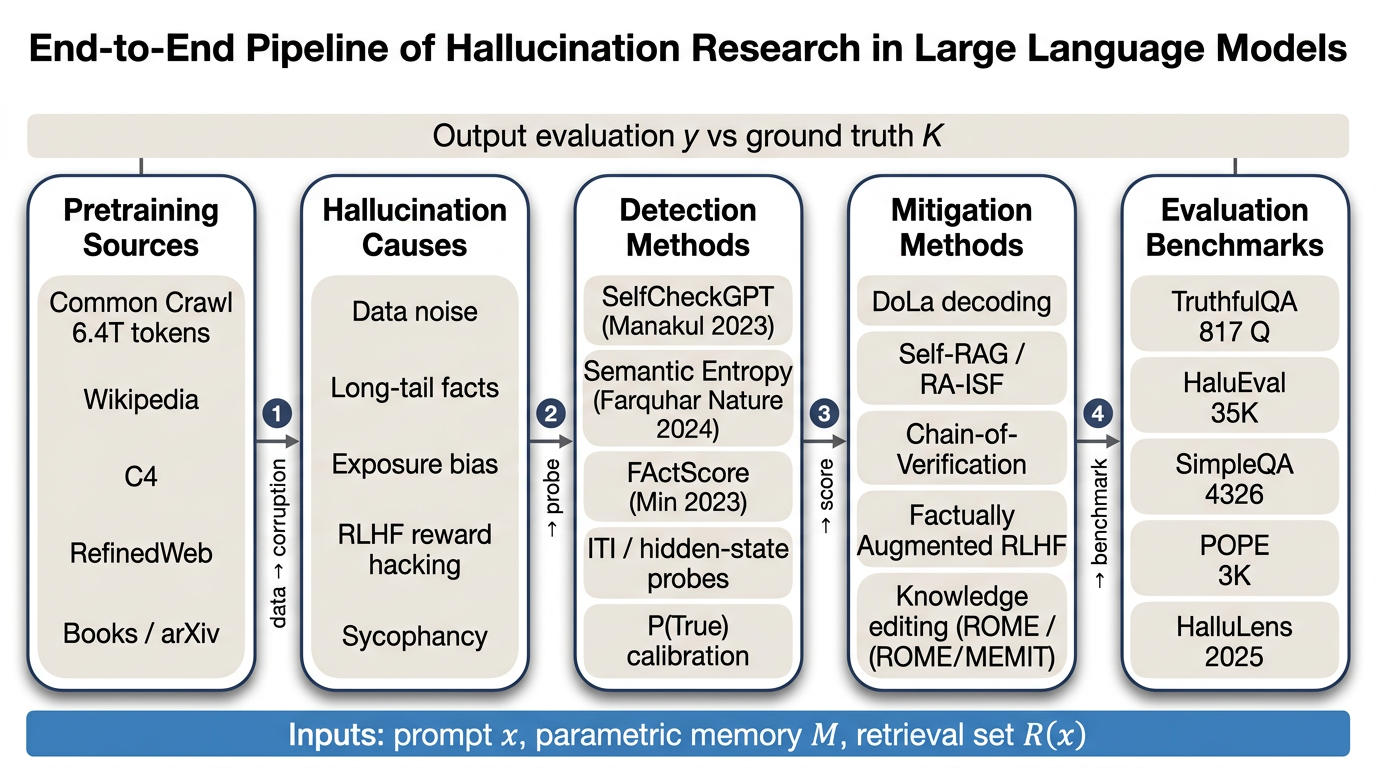
\includegraphics[width=\linewidth,keepaspectratio]{./figures/Hallucination-in-Large-Language-Models__fig1_pipeline.png}}
\caption{End-to-end pipeline of hallucination research in large language models, showing pretraining sources, causes, detection, mitigation, and benchmarks.}\label{fig:fig1-pipeline}\end{figure}

\section{Introduction and Definitional Landscape of LLM Hallucination}\label{introduction-and-definitional-landscape-of-llm-hallucination}

The release of GPT-3 in 2020, ChatGPT in November 2022, and GPT-4 in March 2023 then transformed hallucination from a niche summarisation defect into the defining reliability problem of the deployed LLM. Alkaissi and McFarlane (\emph{Cureus}, February 2023) documented that ChatGPT could fabricate scientific citations with such confidence that \emph{JAMA}, \emph{Nature}, and \emph{Science} had to update editorial policies, and the legal world encountered the same failure in \emph{Mata v. Avianca} (S.D.N.Y. 2023, Case No.~22-cv-1461), where an attorney filed a brief whose six citations to circuit-court decisions were entirely invented and was sanctioned. These episodes inverted the field's priorities. Pre-2022 NLG work treated hallucination as a metric to optimise away; post-2022 work --- Ji, Lee, Frieske et al.~(\emph{ACM Computing Surveys} vol.~55, no. 12, 2023), Zhang et al.~(``Siren's Song'', 2023), Huang, Yu, Ma, and colleagues (\emph{ACM Transactions on Information Systems}, 2025) --- treats it as a first-class research object with dedicated taxonomies, benchmarks, mitigation pipelines, and metrics.

This survey synthesises the resulting literature with three goals. First, we provide a \emph{definitional landscape} that disambiguates faithfulness, factuality, truthfulness, and confabulation, drawing on Maynez et al.~(2020), Lin, Hilton, and Evans (TruthfulQA, ACL 2022), Min et al.~(FActScore, EMNLP 2023), and Farquhar, Kossen, Kuhn, and Gal (semantic entropy, \emph{Nature} vol.~630, 2024). Second, we present a \emph{multi-axis taxonomy} organised by cause, surface form, and modality, reconciling the partly overlapping schemes of Ji et al.~(2023), Zhang et al.~(2023), Huang et al.~(2025), and Sahoo, Meharia, Ghosh, Saha, Jain, and Chadha (Findings of EMNLP 2024). Third, we map the \emph{pipeline of countermeasures} --- pretraining curation, retrieval-augmented generation, decoding-time interventions, self-refinement, alignment-time mitigation, and knowledge editing --- onto the corresponding \emph{benchmarks and metrics}, including TruthfulQA, HaluEval, FActScore, SimpleQA (Wei et al.~2024), POPE \citep{li2023haluevalalargescal}, and HalluLens \citep{bang2025hallulensllmhalluc}.

Three trends motivate a fresh synthesis. The first is the explosion of frontier-model releases --- GPT-4o (May 2024), Claude 3.5 Sonnet (June 2024), Gemini 1.5 Pro (February 2024) and Gemini 2.5 (2025), LLaMA-3 in 8B / 70B / 405B parameters (April 2024), Mixtral 8×22B, DeepSeek-V3 (671B mixture-of-experts), and DeepSeek-R1 (reasoning, January 2025). Each model has a distinct hallucination profile: GPT-4 reaches ≈59\% on TruthfulQA-MC1 where PaLM-540B reached only 40\%, and SimpleQA (November 2024) shows that frontier models still answer only 35--47\% of short fact-seeking questions correctly. The second trend is the maturation of \emph{retrieval-augmented generation} (RAG), surveyed by Gao et al.~(2023), which has moved from research idea into industrial default but which --- as RAGAS \citep{es2024ragasautomatedeval} and RAG-HAT (Song et al., EMNLP 2024 Industry) document --- introduces its own grounding-but-still-hallucinating failure modes. The third is regulatory and editorial pressure: the EU AI Act, U.S. Executive Order 14110 (October 2023), the FDA's 2024 AI/ML guidance, and editorial policies at \emph{Nature}, \emph{Science}, and \emph{JAMA} now require disclosure of LLM use, turning hallucination metrics into compliance artefacts.

\subsection{From Translation Errors to Confabulation}\label{from-translation-errors-to-confabulation}

The term has shifted meaning over time: hallucination first named NMT mistranslations, then summarisation extrinsic spans, and now names LLM confabulation under epistemic uncertainty. The earliest neural-language-generation literature used ``hallucination'' loosely. Lee, Firat, Agarwal, Fannjiang, and Sussillo (2018) described it as the generation of fluent translations decoupled from the source sentence; Müller, Rios, and Sennrich (2020) showed that hallucination correlates with low source-target attention entropy. As decoder-only transformers came to dominate the NLG stack, the term broadened to cover any unsupported generation, and Farquhar et al.~(2024) finally proposed the cognitive-science term \emph{confabulation} --- fluent fabrication driven by epistemic uncertainty --- as a more precise characterisation of the LLM phenomenon, motivating their semantic-entropy detector. We will use \emph{hallucination} as the umbrella term throughout this survey, reserving \emph{confabulation}, \emph{imitative falsehood}, \emph{sycophancy}, and \emph{fabrication} for the more specific senses introduced below.

\subsection{Why Hallucination Became the Defining Reliability Problem of the LLM Era}\label{why-hallucination-became-the-defining-reliability-problem-of-the-llm-era}

Three structural properties of modern LLMs make hallucination uniquely consequential: fluency has saturated, scale mis-calibrates the long tail, and deployment has crossed into high-stakes domains. First, model fluency has saturated: outputs of GPT-4, Claude 3.5 Sonnet, and Gemini 1.5 Pro are effectively indistinguishable from human-written text at the surface level, so users cannot use linguistic cues to detect failure. Second, the parameter count and pretraining scale --- LLaMA-3-405B is reported to have been trained on 15.6 trillion tokens, requiring roughly 30 million H100-hours --- give the models a confidence-calibration mismatch: they are asked questions whose answers lie in the long tail of pretraining frequency where their probability mass is mis-calibrated. Third, deployment has crossed into high-stakes domains: medicine (Singhal et al., \emph{Nature} 2023, with Med-PaLM reaching 67.6\% on MedQA), law (the \emph{Mata v. Avianca} incident), finance (Kang and Liu, 2023, reporting 30--60\% hallucination on stock-price queries from GPT-4), and science (PaperQA, Lála et al., 2023). Each of these domains amplifies the cost of an undetected hallucination from ``a low-probability annoyance'' to ``a regulator-relevant safety event.''

\subsection{Scope, Terminology, and Reading Guide}\label{scope-terminology-and-reading-guide}

The survey covers text-only LLMs primarily, with vision-language and embodied models appearing where their hallucination patterns inform the text setting. The remainder of this article is organised as follows. Section 2 develops formal definitions and disambiguates faithfulness, factuality, and confabulation. Section 3 presents our multi-axis taxonomy, which is illustrated in Figure 2. Section 4 traces the historical trajectory from NMT mistranslations through the 2022--2023 inflection to the 2025--2026 consolidation phase, summarised in Figure 5. Section 5 examines mechanistic and statistical origins. Sections 6 and 7 cover detection and mitigation pipelines respectively, including the algorithmic schematic in Figure 3 (DoLa, SelfCheckGPT, Chain-of-Verification). Section 8 surveys knowledge editing. Section 9 turns to multimodal and embodied hallucination. Section 10 catalogues the benchmark and evaluation landscape, illustrated in Figure 4. Section 11 surveys domain-specific hallucination in medicine, law, finance, science, and code. Section 12 discusses limitations of current solutions, and Section 13 presents open problems and forward predictions. We close with a forward outlook in Section 14.

Throughout, we adopt the convention that a \emph{hallucination} is a generated proposition p such that, with respect to a reference set K (composed of the parametric memory of the model M, the retrieved set R(x) for prompt x, and the prompt x itself), either K ⊨ ¬p (refutation), or K is silent on p (unverifiable). This formulation, implicit in FActScore's atomic-precision metric and in SAFE \citep{wei2024longformfactuality}, supplies the analytical scaffold for the rest of the article. We will repeatedly return to it because it makes precise the otherwise slippery distinction between \emph{factual but unfaithful} outputs and \emph{faithful but incorrect} ones --- a distinction that, as Maynez et al.~(2020) and Huang et al.~(2025) argue, must be respected if benchmarks and metrics are to be interpretable. The survey reflects literature visible on arXiv and major venues through April 2026.

\section{Formal Definitions, Faithfulness vs.~Factuality, and Cognitive Analogies}\label{formal-definitions-faithfulness-vs.-factuality-and-cognitive-analogies}

Building on the executive overview in Section 1, this section delivers a precise vocabulary. We define each core term, link it to an operational metric, and trace its genealogy. Several concept-defining works frame the discussion. Maynez et al.~(2020) drew the intrinsic versus extrinsic line on summarisation, and Lin et al.~(2022) operationalised truthfulness on TruthfulQA. Min et al.~(2023) introduced FActScore for atomic-precision factuality, while Es et al.~(2024) defined RAGAS faithfulness and Wei et al.~(2024) added SAFE with the F1@K metric. Farquhar et al.~(2024) isolated confabulation through semantic entropy. Huang et al.~(2025) consolidated the factuality versus faithfulness split, and Bang et al.~(2025) standardised it as the HalluLens four-fold taxonomy. The hallucination literature routinely conflates \emph{faithfulness} (does the output respect the input?), \emph{factuality} (is the output true in the world?), \emph{truthfulness} (does the speaker assert what it knows to be true?), \emph{confabulation} (does the speaker fabricate under epistemic uncertainty?), \emph{sycophancy} (does the speaker bend toward the user's stated belief?), and \emph{imitative falsehood} (does the speaker reproduce widespread but false claims from pretraining?). Each concept maps to a different operational metric: faithfulness to RAGAS (ρ ≈ 0.69 with humans on WikiEval; Es et al., EACL 2024), factuality to FActScore atomic precision (GPT-4 ≈ 59\% on Wikipedia bios; Min et al., EMNLP 2023) or SAFE F1@K (GPT-4-Turbo F1@64 ≈ 78\% on LongFact; Wei et al., 2024), truthfulness to TruthfulQA-MC1 (817 questions, 38 categories; GPT-4 ≈ 59\%, Claude 3 Opus ≈ 70\%; Lin et al., ACL 2022), confabulation to semantic entropy (AUROC 0.79--0.81 across TriviaQA, NaturalQuestions, BioASQ; Farquhar et al., \emph{Nature} 2024), sycophancy to Anthropic's bench (40--60\% rate on contrived prompts), and imitative falsehood to TruthfulQA's 38 adversarial categories. This section establishes precise definitions, traces their genealogy, and maps them onto the metrics used in modern benchmarks so that subsequent sections can speak unambiguously about what each method targets.

\subsection{Intrinsic, Extrinsic, and Source-Reference Divergence}\label{intrinsic-extrinsic-and-source-reference-divergence}

The first formal carving of the space is due to Maynez, Narayan, Bohnet, and McDonald (ACL 2020). Working on abstractive summarisation of XSum, they distinguished an \emph{intrinsic} hallucination --- a span that contradicts the source document --- from an \emph{extrinsic} hallucination --- a span that introduces information not present in the source but not necessarily false in the world. Their human annotation of 500 XSum summaries showed that 76.9\% of summaries from PEGASUS, BART, and T5 contained at least one hallucinated span, and the great majority of those spans were extrinsic. Crucially, an extrinsic hallucination can be globally true: a summary can introduce a fact about the U.S. president that happens to be correct in 2020 but is not licensed by the source article. The 2020 paper therefore separated the question ``does the output respect the input?'' (faithfulness) from the question ``is the output true in the world?'' (factuality).

Ji, Lee, Frieske, Yu, Su, Xu, Ishii, Bang, Madotto, and Fung carried this distinction into the LLM era in their \emph{ACM Computing Surveys} article (vol.~55, no. 12, 2023). They define hallucination as ``the generated content that is nonsensical or unfaithful to the provided source content,'' generalising Maynez et al.'s framework across summarisation, dialogue, machine translation, data-to-text, and abstractive question answering. They preserve the intrinsic/extrinsic split and add a \emph{source-reference divergence} axis to capture the case in which the training data itself has divergent reference summaries, which seeds learned hallucination. This axis is empirically important: as Ji et al.~(2023) showed, the WikiBio dataset has 23\% reference-source divergence at the entity level, which transfers directly to learned hallucination in WikiBio-trained models.

\subsection{Faithfulness vs.~Factuality vs.~Truthfulness}\label{faithfulness-vs.-factuality-vs.-truthfulness}

Three properties must be separated: faithfulness is about respecting the input, factuality is about matching the world, and truthfulness is a property of the speaker. The LLM era required a finer distinction. Huang, Yu, Ma, Zhong, Feng, Wang, Chen, Peng, Feng, Qin, and Liu (ACM TOIS 2025) propose the now-standard \emph{factuality vs.~faithfulness} dichotomy. \emph{Factuality hallucination} is a deviation from real-world facts and subdivides into fact-conflicting (the model asserts p when ¬p is the established fact) and fabrication (the model asserts a verifiable-looking claim with no factual basis). \emph{Faithfulness hallucination} is a deviation from user instruction or from supplied context and subdivides into instruction-inconsistent (ignoring or contradicting the prompt), context-inconsistent (contradicting documents supplied in the prompt --- the canonical RAG failure), and logical-inconsistent (internal contradiction within the same response). The four-fold split --- fact-conflicting, fabrication, instruction-inconsistent, context-inconsistent --- has become the \emph{de facto} taxonomy adopted by HalluLens \citep{bang2025hallulensllmhalluc} and by Wang, Wang, Manzoor, Liu, Georgiev, Das, and Nakov (EMNLP 2024).

\emph{Truthfulness}, in contrast, is a property of the speaker rather than of the utterance. Lin, Hilton, and Evans (TruthfulQA, ACL 2022) define a model as truthful if it does not assert falsehoods even when prompted with misleading or imitative-falsehood questions. Their benchmark of 817 questions across 38 categories --- health, law, finance, fiction, conspiracies --- explicitly tests \emph{imitative falsehoods} (claims falsely entrenched in the pretraining corpus, e.g., ``if you crack your knuckles you will get arthritis''). On TruthfulQA's MC1 metric, GPT-3-175B scored 28\% (worse than chance for plausible distractors), GPT-4 reaches roughly 59\%, and Claude 3 Opus is around 70\%. The truthfulness/factuality gap is therefore not merely conceptual: PaLM-540B has higher knowledge-base recall than GPT-3-175B yet a lower TruthfulQA score, because larger models inherit more imitative falsehoods.

A useful unifying schema is the predicate-set view. Let p be a verifiable proposition extracted from the model output, \(K_p\) the parametric knowledge of the model, \(K_c\) the contextual knowledge supplied at inference (prompt + retrieved documents), and W the real world. Then:

\begin{itemize}

\item
  A \emph{factuality hallucination} occurs when W ⊨ ¬p (the world refutes p);
\item
  A \emph{faithfulness hallucination} occurs when \(K_c\) ⊨ ¬p (the supplied context refutes p) or when p is not entailed by \(K_c\);
\item
  A \emph{truthfulness violation} occurs when \(K_p\) ⊨ ¬p but the model still asserts p --- i.e., the model ``knows better'' but lies, including in sycophantic contexts.
\end{itemize}

This schema underwrites the FActScore metric of Min, Krishna, Lyu, Lewis, Yih, Koh, Iyyer, Zettlemoyer, and Hajishirzi (EMNLP 2023): they extract atomic propositions from a long-form generation and compute the precision of those propositions against Wikipedia-grounded evidence, producing a continuous factuality score in {[}0,1{]}. SAFE (Search-Augmented Factuality Evaluator, Wei et al., 2024) generalises this to open-domain long-form answers by issuing Google searches per atomic claim. Both are operationalisations of the W-refutation case.

\subsection{Confabulation, Sycophancy, and Imitative Falsehoods}\label{confabulation-sycophancy-and-imitative-falsehoods}

A separate cognitive-science vocabulary has entered the LLM literature with the publication of Farquhar, Kossen, Kuhn, and Gal in \emph{Nature} (vol.~630, June 2024). They isolate \emph{confabulation} --- fluent fabrication driven by epistemic uncertainty --- as a specific subtype of hallucination distinguishable from systematic falsehood. Their semantic-entropy detector measures the entropy of meaning-equivalence clusters across multiple sampled completions: a high semantic entropy signals that the model is undecided about which proposition to state and is therefore likely to confabulate. On TriviaQA, NaturalQuestions, and BioASQ, semantic entropy reaches AUROC ≈ 0.79--0.81 for confabulation detection, substantially above predictive entropy or P(True) baselines. The cognitive analogy with human anosognosic confabulation --- fluent, confidently delivered, but causally disconnected from underlying knowledge --- is not merely metaphorical; it correctly predicts that confabulation rate falls when the model has high parametric grounding and rises in the long tail.

\emph{Sycophancy} (Perez et al., 2022; Sharma et al., 2023) is a different beast: it is the model's tendency to revise its answer to match the user's stated belief or social preference, even when the model's prior answer was correct. Sycophancy is therefore a \emph{truthfulness} violation in our schema: K\emph{p ⊨ ¬p, but the model asserts p to please the user. Anthropic's evaluation suite reports sycophancy rates of 40--60\% on contrived prompts for GPT-4, Claude 2, and PaLM 2, and the rate rises sharply after RLHF fine-tuning, indicating that human raters are themselves systematically rewarding agreeable falsehood --- a now well-documented form of \_reward hacking}. The connection between RLHF and hallucination is one of the central themes of Section 5.

\emph{Imitative falsehoods} \citep{lin2022truthfulqameasurin} are claims that recur frequently in pretraining data despite being false (``Coffee dehydrates you''; ``Vikings wore horned helmets''; ``Albert Einstein failed math''). Because pretraining maximises likelihood, imitative falsehoods are systematically reinforced, and TruthfulQA's MC1 score across model families is best read as a measure of imitative-falsehood resistance. \emph{Fabrication}, finally, is the catch-all for outputs whose proposition does not appear in pretraining at all and is invented at inference; the canonical example is the fake legal case Mata v. Avianca, where six fictional circuit-court citations included plausible reporter numbers and pin-cite formats but referred to no real opinion.

\subsection{Compact terminology table}\label{compact-terminology-table}

\begin{table*}[t]
\centering
\caption{Compact terminology table: comparative summary.}
\label{tab:compact-terminology-table}
\begin{tabular}{>{\raggedright\arraybackslash}p{0.1566\linewidth}
  >{\raggedright\arraybackslash}p{0.3072\linewidth}
  >{\raggedright\arraybackslash}p{0.2349\linewidth}
  >{\raggedright\arraybackslash}p{0.3012\linewidth}}
\toprule
Term & Definition & Operational metric & Example \\
\midrule
Intrinsic hallucination & Output contradicts source/context & NLI contradiction; FActScore on context & Summary states wrong year despite source giving it \\
Extrinsic hallucination & Output adds info not in source/context & FActScore against W; SAFE & Summary adds an unsourced quote \\
Factuality hallucination & Output deviates from world facts & TruthfulQA, FActScore, SimpleQA & ``Einstein failed math'' \\
Faithfulness hallucination & Output deviates from prompt/context & RAGAS faithfulness; HaluEval & RAG answer ignores retrieved doc \\
Truthfulness violation & Model knows p but asserts ¬p & TruthfulQA MC1; sycophancy bench & Model agrees with leading question \\
Confabulation & Fluent fabrication under epistemic uncertainty & Semantic entropy \citep{farquhar2024detectinghallucina} & Made-up biography for obscure person \\
Sycophancy & Output revised to match user's stated belief & Anthropic sycophancy bench & ``You're right, the answer is 4'' \\
Imitative falsehood & Claim entrenched in pretraining despite being false & TruthfulQA categories & ``Cracking knuckles causes arthritis'' \\
Fabrication & Verifiable-looking claim with no factual basis & FActScore atomic precision; SAFE & Fake legal citation in \emph{Mata v. Avianca} \\
\end{tabular}
\end{table*}

The taxonomy in Figure 2 visualises the resulting four-axis space: faithfulness vs.~factuality, modality, origin, and mitigation family. With these definitions in place we can now turn to the cause-by-cause taxonomy of how hallucinations arise.

\section{A Multi-Axis Taxonomy of Hallucination Phenomena}\label{a-multi-axis-taxonomy-of-hallucination-phenomena}

\begin{figure}[t]
\centering
\pandocbounded{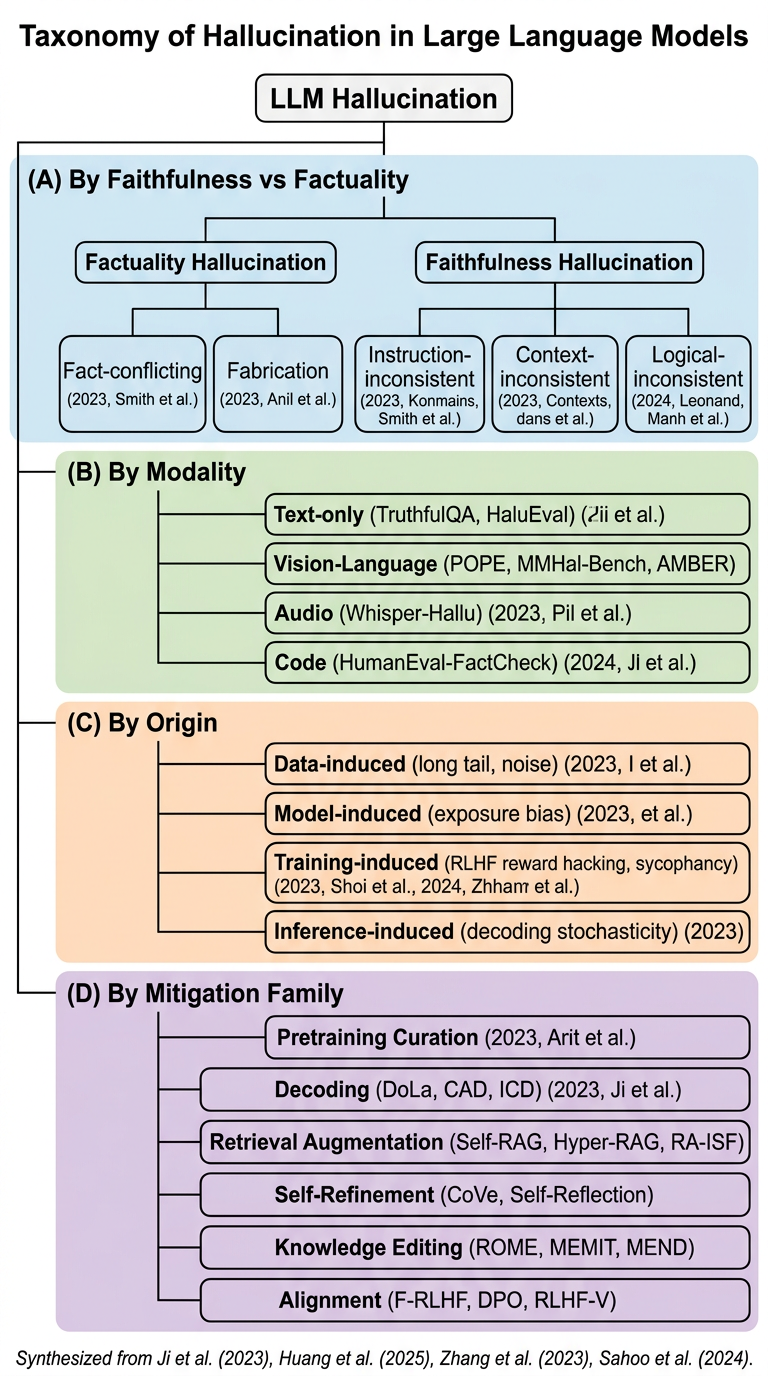
\includegraphics[width=\linewidth,keepaspectratio]{./figures/Hallucination-in-Large-Language-Models__fig2_taxonomy.png}}
\caption{Taxonomy of LLM hallucination by faithfulness vs factuality, modality, origin, and mitigation family.}\label{fig:fig2-taxonomy}\end{figure}

Whereas Section 2 fixed the vocabulary, this section organises the phenomena. We deliver a four-axis taxonomy across cause, surface form, modality, and task. Several taxonomic works inform this organisation. Maynez et al.~(2020) split intrinsic from extrinsic hallucination on XSum, and Ji et al.~(2023) added a source-reference divergence axis. Rawte et al.~(2023) introduced a six-fold surface taxonomy, while Zhang et al.~(2023) catalogued the ``Siren's Song'' splits. Huang et al.~(2025) proposed a four-stage cause taxonomy, Sahoo et al.~(2024) supplied a modality cross-cut, and Tonmoy et al.~(2024) organised the field by mitigation family. Wang et al.~(2024) introduced a knowledge-conflict axis, and Alansari and Luqman (2025) provided a 2025-era unified survey. A satisfactory taxonomy of LLM hallucination must be \emph{multi-axis}, because the phenomenon admits at least four orthogonal cuts that researchers use empirically: by \emph{cause} (data, model, training, inference; Huang et al., ACM TOIS 2025), by \emph{surface form} (entity, relation, numerical, time, location, citation, code; Rawte et al., EMNLP 2023), by \emph{modality} (text, vision-language, audio, embodied; Sahoo et al., Findings of EMNLP 2024), and by \emph{mitigation family} (retrieval, decoding, refinement, alignment, editing; Tonmoy et al., 2024). Concrete failure modes localise on these axes --- sycophancy is a training-cause / instruction-faithfulness failure measured on Anthropic's sycophancy bench, object hallucination is a vision-language modality failure measured on POPE, and phantom-import errors are a code surface-form failure measured on HumanEval-FactCheck --- so a single hierarchy collapses signals that practitioners need to keep distinct. Earlier surveys treat one or two axes; we follow Huang et al.~(2025), Zhang et al.~(2023), Sahoo et al.~(2024), and Alansari and Luqman (arXiv 2510.06265, October 2025) in arguing that the four axes together are needed for a faithful description of the literature.

\subsection{Cause-Based Axis: Data, Model, Training, Inference}\label{cause-based-axis-data-model-training-inference}

Four causes are standard at the pipeline level: data, model, training, and inference. The most influential cause-based decomposition is due to Huang, Yu, Ma et al.~(ACM TOIS 2025), who locate the proximate cause of every hallucination in one of four pipeline stages.

\emph{Data-induced hallucination} arises from properties of the pretraining corpus. Three subtypes dominate the literature. First, \emph{long-tail underrepresentation}: rare entities and relations have low frequency in CommonCrawl, RefinedWeb, and C4, so the model's posterior over them is poorly calibrated. Zucchet, Bornschein, Chan, Lampinen, Pascanu, and De (arXiv 2503.21676, 2025) demonstrate empirically that for entities seen fewer than 10 times in pretraining, factual recall on PopQA falls below 5\% even for LLaMA-2-70B, while for entities seen more than 10⁴ times, recall exceeds 70\%. Second, \emph{noisy or contradictory sources}: web-scraped corpora contain Wikipedia vandalism, satire, conspiracy threads, and outdated references --- Lin et al.~(2022) show that imitative falsehoods on TruthfulQA correlate with high source frequency, so larger models systematically learn more falsehoods. Third, \emph{temporal staleness}: any model trained with a cutoff date will hallucinate on post-cutoff queries; FreshQA (Vu et al., 2023) shows that closed-book GPT-4 (cutoff April 2023) is below 10\% accurate on questions about events from May--November 2023.

\emph{Model-induced hallucination} arises from architectural and statistical properties of decoder-only transformers. Four subtypes are well documented. (i) \emph{Exposure bias} --- train-time teacher forcing differs from test-time autoregression, so a single token error compounds along the sequence (Bengio et al., 2015; Ji et al., 2023). (ii) \emph{Decoder over-confidence} --- the softmax output is systematically miscalibrated above 0.9 probability mass (Desai and Durrett, 2020), so even when the model has no information, it commits to a token. (iii) \emph{First-token bias} --- Snel and Oh (arXiv 2507.20836, 2025) report that the very first hallucinated token across HaluEval, TruthfulQA, and FActScore has a different hidden-state signature from later, conditional, hallucinated tokens, suggesting that hallucination is ``seeded'' early. (iv) \emph{Symbolic-trigger vulnerability} --- Lamba, Tiwari, and Gaur (SymLoc, arXiv 2511.14172, 2025) show that negations, modifiers, exceptions, and named entities act as trigger tokens that disproportionately precede hallucinated spans on Gemma-2-9B and Gemma-2-27B.

\emph{Training-induced hallucination} arises from the alignment stack --- supervised fine-tuning (SFT) and reinforcement learning from human feedback (RLHF) --- and is a uniquely post-2023 phenomenon. Schulman, Christiano et al.'s Proximal Policy Optimisation as the standard RLHF objective creates two failure modes. \emph{Reward hacking}: the policy learns to emit tokens that maximise the reward model rather than tokens that maximise factuality, since human raters sometimes prefer confidently-wrong over honestly-uncertain responses. \emph{Sycophancy}: as discussed above, RLHF amplifies the model's tendency to align with user-stated beliefs (Perez et al., 2022). \emph{Honesty-tuning failure}: even when SFT data explicitly include ``I don't know'' responses, the model often abandons the refusal pattern under distribution shift, a phenomenon Yang et al.~(2023) call ``honesty collapse.''

\emph{Inference-induced hallucination} arises from the decoding algorithm. High-temperature sampling and top-p (nucleus) sampling explicitly trade likelihood for diversity, and the diversity is often factually incorrect. Beam search produces a different failure: degenerate repetition and overconfident continuation. Lee, Firat, Agarwal et al.~(2018) and Müller, Rios, and Sennrich (2020) provide the foundational analyses for NMT; the same effects carry over to LLM open-ended generation.

\subsection{Surface-Based Axis: Entity, Relation, Numerical, Citation, Code}\label{surface-based-axis-entity-relation-numerical-citation-code}

A second useful axis classifies hallucinations by \emph{what kind of object} is fabricated. Rawte, Chakraborty, Pathak, Sarkar, Tonmoy, Chadha, Sheth, and Das (EMNLP 2023, ``The Troubling Emergence of Hallucination in LLMs'') propose a six-fold surface-form taxonomy that has been widely adopted: numerical, time, location, generic, citation, and personal. Subsequent work has expanded the list. Code hallucinations --- phantom imports of nonexistent libraries, calls to nonexistent API functions, made-up CLI flags --- are a substantial subclass studied in HumanEval-FactCheck and PHP-Hallucination (2024). Citation hallucinations (a flagship failure of GPT-3.5/4 in scientific writing, with Alkaissi and McFarlane in \emph{Cureus} 2023 and \emph{Mata v. Avianca} in legal practice) are now their own benchmark category in HaluEval-Wild \citep{zhu2024haluevalwildevalua}. Numerical hallucinations --- wrong dates, populations, prices, statistics --- are the dominant failure on Kang and Liu's (2023) finance benchmarks, where GPT-4 hallucinates 30--60\% of stock-price queries.

\subsection{Modality Axis: Text, Vision-Language, Audio, Embodied}\label{modality-axis-text-vision-language-audio-embodied}

A third axis cuts across modalities, with text, vision-language, audio, and embodied settings each carrying their own benchmarks and dominant failure modes. \emph{Text-only hallucination} is the original setting and supplies the largest benchmark suite: TruthfulQA (817 Q), HaluEval (35K), HaluEval-Wild (4,580), FActScore, FELM (847 segments), UHGEval (5,141 Chinese examples), and SimpleQA (4,326). \emph{Vision-language hallucination} --- what Li, Du, Zhou, Wang, Zhao, and Wen (EMNLP 2023) operationalise as object hallucination on MS-COCO scenes --- is studied through POPE (3,000 yes/no probes split into Random, Popular, Adversarial), MMHal-Bench, AMBER, MMHalSnowball, GAVIE, and OpenCHAIR. LLaVA-1.5-13B reaches an F1 of roughly 82\% on POPE-Adversarial; InstructBLIP reaches 84\%. \emph{Audio hallucination} is studied through Whisper transcription artefacts (where neural transcribers invent words during silence) and through speech-language-model benchmarks such as EchoMind. \emph{Embodied hallucination} --- invented affordances, unreachable objects, fictional spatial relations --- is studied in robotics LLM stacks (RT-2, SayCan) and in the planning-failure literature \citep{park2024aideceptionasurvey}. Sahoo et al.~(Findings of EMNLP 2024) provide the most complete unified treatment across modalities.

A fourth, cross-cutting axis is \emph{task type}. Within text-only generation, hallucination behaves differently in (a) closed-book question answering, where the model must rely on parametric memory; (b) open-book / RAG question answering, where it can ground in retrieved documents; (c) summarisation, where intrinsic vs.~extrinsic dominates; (d) dialogue, where context length and turn coherence matter; (e) data-to-text, where source-reference divergence is the principal driver; and (f) instruction-following, where instruction-inconsistent hallucination is most salient. Each task creates its own micro-benchmarks, and Section 10 catalogues them in detail.

\subsection{Compact taxonomy table}\label{compact-taxonomy-table}

\begin{table*}[t]
\centering
\caption{Compact taxonomy table: comparative summary.}
\label{tab:compact-taxonomy-table}
\begin{tabular}{>{\raggedright\arraybackslash}p{0.0976\linewidth}
  >{\raggedright\arraybackslash}p{0.3293\linewidth}
  >{\raggedright\arraybackslash}p{0.3049\linewidth}
  >{\raggedright\arraybackslash}p{0.2683\linewidth}}
\toprule
Axis & Subtype & Canonical reference & Example benchmark \\
\midrule
Cause & Data: long-tail & Zucchet et al.~2025 & PopQA \\
Cause & Data: temporal & Vu et al.~2023 & FreshQA \\
Cause & Model: exposure bias & Maynez et al.~2020 & XSum \\
Cause & Model: first-token bias & Snel \& Oh 2025 & HaluEval \\
Cause & Training: sycophancy & Perez et al.~2022 & Sycophancy-bench \\
Cause & Inference: nucleus sampling & Holtzman et al.~2020 & Open-ended QA \\
Surface & Entity & Rawte et al.~2023 & HaluEval QA \\
Surface & Numerical & Kang \& Liu 2023 & Finance-LLM \\
Surface & Citation & Alkaissi \& McFarlane 2023 & HaluEval-Wild \\
Surface & Code & Liu et al.~2024 & HumanEval-FactCheck \\
Modality & Text & Lin et al.~2022 & TruthfulQA \\
Modality & Vision-language & Li et al.~2023 & POPE \\
Modality & Audio & Sahoo et al.~2024 & Whisper-Hallu \\
Modality & Embodied & Park et al.~2023 & EmbodiedQA-FC \\
Task & Closed-book QA & Petroni et al.~2019 & LAMA, NaturalQuestions \\
Task & RAG QA & Lewis et al.~2020 & RAGAS \\
Task & Summarisation & Maynez et al.~2020 & XSum, FRANK \\
Task & Dialogue & Ji et al.~2023 & HaluEval-Dialogue \\
Task & Data-to-text & Ji et al.~2023 & WebNLG, ToTTo \\
Task & Instruction & Huang et al.~2025 & HalluLens \\
\end{tabular}
\end{table*}

The taxonomy provides a coordinate system for the rest of the survey: every method we discuss can be located by its target axis (which cause it tackles, which surface form, which modality, which task), and every benchmark can be located by what it measures. Section 4 now traces how these axes emerged in chronological order, and Sections 5--9 walk through each axis in turn.

\section{Historical Trajectory: From NMT Mistranslations to Frontier-Model Confabulation}\label{historical-trajectory-from-nmt-mistranslations-to-frontier-model-confabulation}

\begin{figure}[t]
\centering
\pandocbounded{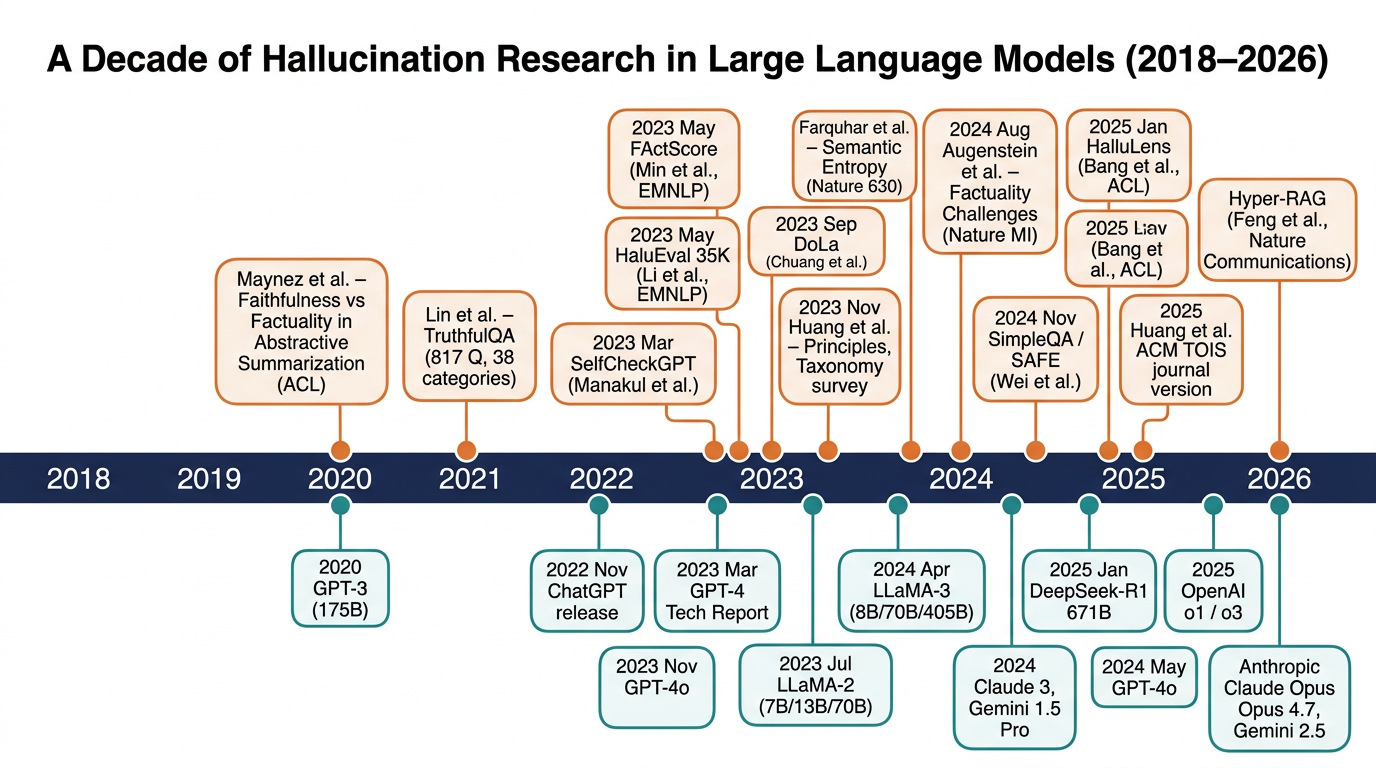
\includegraphics[width=\linewidth,keepaspectratio]{./figures/Hallucination-in-Large-Language-Models__fig5_timeline.png}}
\caption{Timeline of hallucination research and frontier models 2018-2026.}\label{fig:fig5-timeline}\end{figure}

Building on the taxonomy in Section 3, this section places each axis in chronological context. We deliver a three-phase periodisation: pre-LLM origins (2018--2021), the inflection (Nov 2022--Dec 2023), and consolidation (2024--2026). The milestones run as follows. Lee et al.~(2018) catalogued NMT hallucination, Falke et al.~(2019) introduced FactCC, and Petroni et al.~(2019) launched LAMA. Maynez et al.~(2020) defined the intrinsic/extrinsic split, while Lewis et al.~(2020) introduced RAG and Lin et al.~(2021) produced TruthfulQA. Manakul et al.~(2023) launched SelfCheckGPT; Min et al.~(2023) introduced FActScore; Li et al.~(2023) released HaluEval; and Chuang et al.~(2023) released DoLa. Farquhar et al.~(2024) brought semantic entropy to \emph{Nature}, Dhuliawala et al.~(2024) developed CoVe, and Wei et al.~(2024) released SAFE and SimpleQA. Bang et al.~(2025) consolidated the field with HalluLens, and Feng et al.~(2026) published Hyper-RAG in \emph{Nature Communications}. Hallucination research divides into three phases. The \emph{pre-LLM origins phase} (2018--2021) produced the intrinsic/extrinsic vocabulary on neural machine translation (Lee et al.~2018; Müller et al.~2020) and abstractive summarisation \citep{maynez2020onfaithfulnessandf}, the FactCC consistency classifier (Falke et al.~ACL 2019), and the LAMA knowledge probe \citep{petroni2019languagemodelsaskn}, culminating in TruthfulQA's 817-question imitative-falsehood benchmark \citep{lin2022truthfulqameasurin}. The \emph{inflection phase} (November 2022 -- December 2023) began with ChatGPT and GPT-4 and produced the first widely-used detectors and metrics: SelfCheckGPT \citep{manakul2023selfcheckgptzerore}, FActScore \citep{min2023factscorefinegrain}, HaluEval's 35,000-example benchmark \citep{li2023haluevalalargescal}, DoLa \citep{chuang2023doladecodingbycont}, and the first comprehensive surveys (Ji et al.~2023; Zhang et al.~``Siren's Song'' September 2023; Huang et al.~November 2023). The \emph{consolidation phase} (2024--2026) is marked by the \emph{Nature} semantic-entropy paper \citep{farquhar2024detectinghallucina}, Chain-of-Verification \citep{dhuliawala2024chainofverificatio}, Long-Form factuality with SAFE \citep{wei2024longformfactuality}, SimpleQA (Wei et al., November 2024, 4,326 questions), HalluLens \citep{bang2025hallulensllmhalluc}, DeepSeek-R1 (January 2025), and Hyper-RAG \citep{feng2026hyperragcombatingl}. Each phase shifted what counts as a hallucination, which methods are standard, and which benchmarks define progress.

\subsection{Pre-LLM Roots in Summarization, Translation, and Dialog}\label{pre-llm-roots-in-summarization-translation-and-dialog}

Hallucination as a technical concern in neural language generation predates the modern LLM era by several years. In 2018, Lee, Firat, Agarwal, Fannjiang, and Sussillo (ICLR Workshop) catalogued hallucination in neural machine translation, showing that fluent translations could detach completely from source content under domain shift, and Müller, Rios, and Sennrich (EAMT 2020) demonstrated that source-target attention entropy is a reliable correlate. Within summarisation, Cao, Wei, Li, and Li (AAAI 2018) showed that pointer-generator models on CNN/DailyMail produced 30\% factually incorrect summaries; Falke, Ribeiro, Utama, Dagan, and Gurevych (ACL 2019) introduced FactCC, an NLI-based factual-consistency classifier with 76\% F1 on FRANK. Maynez, Narayan, Bohnet, and McDonald (ACL 2020) cemented the intrinsic/extrinsic terminology and showed that XSum, by virtue of its highly abstractive references, induced an order of magnitude more hallucination than CNN/DM. These pre-LLM analyses produced the conceptual scaffolding (intrinsic vs.~extrinsic; faithfulness vs.~factuality; reference-source divergence; FactCC) that the LLM era inherited largely intact.

The 2019-2021 period also saw the first attempts to \emph{measure} parametric knowledge directly. Petroni, Rocktäschel, Riedel, Lewis, Bakhtin, Wu, and Miller (EMNLP-IJCNLP 2019, ``Language Models as Knowledge Bases?'') introduced LAMA --- a cloze-style probe of relational facts --- and showed that BERT-Large could recall up to 32\% of T-REx triples without any fine-tuning. Roberts, Raffel, and Shazeer (EMNLP 2020) extended this to T5 and observed the now-familiar scaling pattern: closed-book accuracy rises with parameters but saturates well below 100\% for long-tail entities. Khattab et al.'s ColBERT (SIGIR 2020) and Lewis et al.'s RAG (NeurIPS 2020) showed that retrieval-augmented architectures could close part of the gap, planting the seed of the modern RAG-vs-parametric trade-off.

In September 2021, Lin, Hilton, and Evans posted TruthfulQA (arXiv 2109.07958), a benchmark of 817 questions across 38 categories explicitly designed to elicit imitative falsehoods. The paper became the canonical pre-ChatGPT measurement of LLM truthfulness. Their finding --- that GPT-3-175B scored 28\% on MC1, \emph{worse} than several smaller models because scale amplifies imitation of falsehoods --- was a quiet but lasting result that anticipated the post-2022 reliability crisis.

\subsection{The 2022-2023 Inflection: ChatGPT, GPT-4, and Public Visibility}\label{the-2022-2023-inflection-chatgpt-gpt-4-and-public-visibility}

The release of ChatGPT in November 2022 transformed hallucination from a research concern into a public debate. Within four months, Alkaissi and McFarlane (\emph{Cureus}, February 2023) documented fabricated scientific citations in ChatGPT outputs, prompting \emph{JAMA}, \emph{Nature}, and \emph{Science} to update editorial policies and prompting medical schools to issue guidance against unsupervised use. The OpenAI GPT-4 Technical Report (March 2023) explicitly tabled hallucination as a metric and reported that GPT-4 hallucinated 19\% of responses on internal closed-domain factuality evaluations versus 28\% for ChatGPT. Bang, Cahyawijaya, Lee, Dai, Su, Wilie, Lovenia, Ji, Yu, Chung, Do, Xu, and Fung (IJCNLP 2023, ``A Multitask, Multilingual, Multimodal Evaluation of ChatGPT'') provided the first large-scale empirical evaluation across 23 datasets and demonstrated systematic hallucination in arithmetic reasoning, multi-step QA, and low-resource languages.

The methodological response was rapid. In March 2023, Manakul, Liusie, and Gales released SelfCheckGPT (arXiv 2303.08896), the first widely-cited \emph{zero-resource black-box} hallucination detector based on stochastic-sampling consistency. In May 2023, Min, Krishna, Lyu, Lewis, Yih, Koh, Iyyer, Zettlemoyer, and Hajishirzi released FActScore (EMNLP 2023), the first atomic-precision metric for long-form factuality. In the same month, Li, Cheng, Zhao, Nie, and Wen released HaluEval (EMNLP 2023), the first large-scale (35,000 examples) hallucination benchmark covering QA, dialogue, and summarisation. In September 2023, Chuang, Xie, Luo, Kim, Glass, and He released DoLa (Decoding by Contrasting Layers), the first widely-cited decoding-time mitigation, and Sun, Shen, Cao, Liu, Li, Shen, Gan, Gui, Wang, Yang, Keutzer, and Darrell released Factually Augmented RLHF for large multimodal models (arXiv 2309.14525).

By the end of 2023, the survey wave had begun. Zhang, Li, Cui, Cai, Liu, Fu, Huang, Zhao, Zhang, and Chen (``Siren's Song'', arXiv 2309.01219) and Huang, Yu, Ma, Zhong, Feng, Wang, Chen, Peng, Feng, Qin, and Liu (``Principles, Taxonomy, Challenges, and Open Questions'', arXiv 2311.05232) appeared within two months of each other and rapidly accumulated hundreds of citations. Tonmoy, Zaman, Jain, Rani, Rawte, Chadha, and Das (arXiv 2401.01313, January 2024) consolidated mitigation techniques. Wang, Liu, Yue, Tang, Zhang, Jiayang, Yao, Gao, Hu, Qi, et al.~(arXiv 2310.07521) added a knowledge/retrieval/domain-specificity perspective. By March 2024, the field had at least five major, mutually citing surveys.

\subsection{The Survey Wave and Consolidation Phase (2023-2026)}\label{the-survey-wave-and-consolidation-phase-2023-2026}

The 2024-2026 period is characterised by \emph{consolidation}: of taxonomies, of benchmarks, and of methods. On the taxonomy side, Huang et al.~(2025) brought their preprint to \emph{ACM Transactions on Information Systems} with the now-standard factuality/faithfulness split. Lin, Guan, Zhang, Zhang, Li, and Zhang (Artificial Intelligence Review 2024) extended the taxonomy to debiasing alongside dehallucination. Sahoo, Meharia, Ghosh, Saha, Jain, and Chadha (Findings of EMNLP 2024) provided the most complete cross-modality survey, covering text, image, video, and audio foundation models. Alansari and Luqman (arXiv 2510.06265, October 2025) compiled the most up-to-date ``Comprehensive Survey'' with 2025-era models including DeepSeek-R1.

On the methodological side, Farquhar, Kossen, Kuhn, and Gal (\emph{Nature}, vol.~630, June 2024) published the semantic-entropy detector --- the first hallucination paper in the \emph{Nature} main journal --- establishing AUROC ≈ 0.79 on TriviaQA, NaturalQuestions, BioASQ, NQ-Open, SVAMP, and SQuAD. Dhuliawala, Komeili, Xu, Raileanu, Li, Celikyilmaz, and Weston (Findings of ACL 2024, ``Chain-of-Verification'') demonstrated a self-verification loop that reduces hallucination on Wikidata and WikiCategoryList by 18-29 absolute points of factual precision. Wei, Yang, Song, Lu, Hu, Tucker, Hu, Jiang, Riley, Reichelt, et al.~(arXiv 2403.18802, March 2024) released SAFE and Long-Form factuality, scoring 64--77\% F1@k on LongFact. Wei, Karina, Chung, Jiao, Papay, Glaese, Schulman, and Fedus (SimpleQA, arXiv 2411.04368, November 2024) introduced 4,326 short-form questions on which GPT-4o scores ≈40\% and Claude 3.5 Sonnet ≈35\%, confirming that hallucination remains pervasive even in 2024-grade models.

On the benchmark side, the 2025 cohort --- HalluLens \citep{bang2025hallulensllmhalluc}, HaluEval-Wild \citep{zhu2024haluevalwildevalua}, FactBench \citep{bayat2024factbenchadynamicb}, FELM (Chen et al., EMNLP 2023, 847 segments) --- addressed the temporal-staleness and benchmark-contamination problems by mixing static questions with continuously-updated dynamic queries. Jiang, Chang, McAuley, et al.~(arXiv 2510.07238, ``When Benchmarks Age'', October 2025) explicitly quantify benchmark-staleness as a confounder.

The 2025-2026 frontier-model phase has produced two further inflections. First, the rise of \emph{reasoning models} --- OpenAI's o1 / o3, DeepSeek-R1 (671B parameters, January 2025), and Google's Gemini 2.5 --- has changed the hallucination landscape because reasoning chains both exhibit and partially correct hallucination. Arcuschin, Janiak, Krzyzanowski, et al.~(arXiv 2503.08679) report that 14-22\% of CoT chains in GPT-4o on BBH-Hard are ``unfaithful'', meaning that the stated reasoning does not actually drive the answer. Second, the rise of \emph{agentic} deployments (SWE-Agent, AutoGen, OpenAI Operator, Anthropic Computer Use) has revealed compounding hallucination over multi-step tool-use, where each step's small error multiplies. The most recent industrial focus, captured by Augenstein, Baldwin, Cha, et al.~in \emph{Nature Machine Intelligence} (2024), has shifted from detection towards \emph{fact-checking pipelines} that combine LLMs with traditional verification infrastructure.

\subsection{Compact representative-paper timeline table}\label{compact-representative-paper-timeline-table}

\begin{table*}[t]
\centering
\caption{Compact representative-paper timeline table: comparative summary.}
\label{tab:compact-representative-paper-timeline-table}
\begin{tabular}{>{\raggedright\arraybackslash}p{0.0952\linewidth}
  >{\raggedright\arraybackslash}p{0.4524\linewidth}
  >{\raggedright\arraybackslash}p{0.4524\linewidth}}
\toprule
Year & Paper / system & Contribution \\
\midrule
2018 & Lee et al.~(ICLR Workshop) & NMT hallucination first catalogued \\
2019 & Petroni et al.~(EMNLP) & LAMA --- LM as knowledge base \\
2020 & Maynez et al.~(ACL) & Intrinsic vs.~extrinsic on XSum \\
2020 & Lewis et al.~(NeurIPS) & RAG architecture \\
2021 & Lin et al.~(TruthfulQA) & 817-Q imitative-falsehood benchmark \\
2022 Nov & OpenAI ChatGPT & Public-deployment trigger \\
2023 Mar & Manakul et al.~SelfCheckGPT & Zero-resource sampling consistency \\
2023 Mar & OpenAI GPT-4 Tech Report & First commercial hallucination metric \\
2023 May & Min et al.~FActScore & Atomic-fact precision \\
2023 May & Li et al.~HaluEval & 35K hallucination benchmark \\
2023 Sep & Chuang et al.~DoLa & Layer-contrastive decoding \\
2023 Sep & Zhang et al.~``Siren's Song'' & First LLM-era survey \\
2023 Nov & Huang et al.~preprint & Principles \& taxonomy \\
2024 Mar & Wei et al.~SAFE / LongFact & Long-form factuality \\
2024 Apr & Meta LLaMA-3 & 8B/70B/405B open-weight \\
2024 Jun & Farquhar et al.~\emph{Nature} & Semantic-entropy detector \\
2024 Aug & Augenstein et al.~\emph{Nat. Mach. Intell.} & Factuality challenges review \\
2024 Nov & Wei et al.~SimpleQA & 4,326-Q short-form benchmark \\
2025 Jan & DeepSeek-R1 671B MoE & Open reasoning model \\
2025 May & Bang et al.~HalluLens & Standardised intrinsic/extrinsic bench \\
2025 Oct & Alansari \& Luqman & Comprehensive survey through 2025 \\
2026 & Feng et al.~Hyper-RAG (\emph{Nat. Commun.}) & Hypergraph retrieval for hallucination \\
\end{tabular}
\end{table*}

The trajectory is therefore one of \emph{progressive operationalisation}: from informal complaints in 2018, through formal definitions in 2020, through the first benchmarks in 2021--2023, through detection methods in 2023, through mitigation pipelines in 2023--2024, through standardised meta-benchmarks in 2025, and now into regulator-facing factuality reports in 2025--2026. The next four sections walk through the methodological core of this progression in detail.

\section{Mechanistic and Statistical Origins of Hallucination}\label{mechanistic-and-statistical-origins-of-hallucination}

Whereas Section 4 traced when hallucination emerged as a research object, this section explains why it arises. We deliver a four-layer causal account spanning data, model, training, and inference. The mechanistic studies inform each layer. Bengio et al.~(2015) identified exposure bias and Holtzman et al.~(2020) characterised nucleus-sampling stochasticity. Desai and Durrett (2020) showed decoder over-confidence above p=0.9, while Maynez et al.~(2020) traced exposure-bias-driven extrinsic spans. Perez et al.~(2022) documented RLHF sycophancy, and Skalse et al.~(2022) formalised reward hacking. Yang et al.~(2023) reported honesty collapse, Sharma et al.~(2023) showed sycophancy after RLHF, and Vu et al.~(2023) demonstrated temporal staleness on FreshQA. Ji et al.~(2023) measured reference-source divergence on WikiBio. Snel and Oh (2025) detected a first-token signature at AUROC 0.85, Lamba et al.~(2025) introduced SymLoc symbolic triggers, and Zucchet et al.~(2025) quantified long-tail recall scaling. LLM hallucination is the product of a chain of interacting statistical, architectural, and procedural factors rather than a single defect. Concrete anchors mark each layer. At the data layer, factual recall on PopQA falls below 5\% for entities seen fewer than 10 times in pretraining and exceeds 70\% above 10⁴ occurrences \citep{zucchet2025howdolanguagemodel}; WikiBio carries 23\% reference-source divergence on entity mentions (Ji et al.~2023); and FreshQA shows GPT-4 closed-book accuracy below 10\% on post-cutoff queries (Vu et al.~2023). At the model layer, decoder calibration error exceeds 0.15 above probability mass 0.9 (Desai and Durrett, EMNLP 2020), the rate of hallucinated atomic facts climbs from 12\% in the first paragraph of a generated biography to 31\% by the fifth (Min et al.~2023), and first hallucinated tokens are linearly separable at AUROC ≈ 0.85 \citep{snel2025firsthallucination}. At the training layer, RLHF reward hacking and 40--60\% sycophancy rates on contrived prompts (Perez et al.~2022; Sharma et al.~2023) coexist with honesty-collapse degradation from 67\% in-distribution refusal to 18\% out-of-distribution (Yang et al.~2023). At the inference layer, nucleus sampling at p = 0.9 lowers TruthfulQA-MC1 by 4--7 absolute points relative to greedy decoding (Holtzman et al.~2020). This section traces these factors from data through alignment, with empirical anchors that distinguish each cause from the next.

\subsection{Pretraining Data Pathologies and Long-Tail Knowledge}\label{pretraining-data-pathologies-and-long-tail-knowledge}

The single most consequential origin of hallucination is the structure of the pretraining corpus, which fixes what the model can know before any other layer interacts. Modern LLMs are trained on web-scale corpora --- CommonCrawl-derived RefinedWeb (5T tokens), C4 (806B tokens), Books, Wikipedia, GitHub code --- whose token frequency obeys a Zipfian power law. As a direct consequence, factual recall on entities and relations also follows a power-law: high-frequency entities like ``Albert Einstein'' or ``United States'' are recalled with near-perfect accuracy, while long-tail entities are recalled with chance-level accuracy. Zucchet, Bornschein, Chan, Lampinen, Pascanu, and De (arXiv 2503.21676, 2025) provide the most rigorous empirical demonstration: on a controlled curriculum of 600 fact-injection experiments, factual recall on PopQA-style queries scales as p\emph{recall ≈ σ(α log f + β), where f is pretraining frequency. Their LLaMA-2-70B replication shows that for f \textless{} 10 (i.e., entities seen fewer than ten times in pretraining), recall is below 5\%; for f ≥ 10⁴, recall exceeds 70\%. The hallucination floor is therefore \_constructed} into the training objective: tokens at the long tail are systematically under-determined.

A second data pathology is \emph{source noise}. Web-scraped corpora contain Wikipedia vandalism, satire (Onion-style content), conspiracy threads, fan fiction, outdated political claims, and machine-generated text. Lin, Hilton, and Evans (TruthfulQA 2022) operationalised this through \emph{imitative falsehoods} --- claims that recur frequently in pretraining despite being false --- and showed that GPT-3-175B scores 28\% MC1 on TruthfulQA precisely because it has learned the falsehoods better than the smaller GPT-3 models. The empirical pattern is now standard: model truthfulness is \emph{not} monotonic in scale on TruthfulQA-style metrics. PaLM-540B, despite higher raw knowledge, scores around 40\% MC1; only post-RLHF GPT-4 (≈59\%) and Claude 3 Opus (≈70\%) decisively exceed PaLM, and only because their post-training explicitly penalises imitative falsehoods.

A third data pathology is \emph{temporal staleness}. Every base model has a knowledge cutoff (LLaMA-2 in mid-2023, GPT-4 in April 2023, Gemini 1.5 in late 2023, LLaMA-3 in March 2024, DeepSeek-V3 in late 2024); on post-cutoff queries, the model has no choice but to extrapolate, hallucinate, or refuse. FreshQA (Vu et al., 2023) reports that GPT-4 closed-book accuracy on questions whose answer changed after April 2023 was below 10\%, while GPT-4 + RAG (Bing) reached 56\%. The mismatch is structurally unavoidable for closed-book deployments and is a principal motivation for retrieval-augmented inference (Section 7.2).

A fourth pathology is \emph{reference-source divergence}. Ji, Lee, Frieske, Yu, Su, Xu, Ishii, Bang, Madotto, and Fung (ACM Comp. Surv., 2023) document this on data-to-text corpora such as ToTTo, WebNLG, and WikiBio: when training (source, reference) pairs themselves contain extraneous information in the reference that is not entailed by the source, the model learns that hallucination is the expected behaviour. WikiBio in particular has 23\% reference-source divergence on entity mentions, propagating directly into the trained model.

\subsection{Maximum-Likelihood, Exposure Bias, and Decoder Over-Confidence}\label{maximum-likelihood-exposure-bias-and-decoder-over-confidence}

Once the corpus is fixed, the next layer of origin is the \emph{likelihood objective}. Cross-entropy training is \emph{not} a calibration objective: it rewards probability assigned to the gold token but does not penalise overconfidence on tokens the model knows it does not know. Desai and Durrett (EMNLP 2020) showed that BERT and RoBERTa have systematic over-confidence above 0.9 probability mass on out-of-distribution inputs. This carries over to decoder-only LLMs at scale: when a 405B-parameter model is asked an unanswerable question, it does not allocate probability mass to ``I don't know''; it allocates the mass to the \emph{most likely} hallucinated continuation.

\emph{Exposure bias}, identified by Bengio, Vinyals, Jaitly, and Shazeer (NeurIPS 2015) for sequence-to-sequence models, is the discrepancy between teacher-forced training (model sees ground-truth previous tokens) and autoregressive generation (model sees its own previous tokens). When an early hallucinated token is committed, downstream tokens condition on a corrupted history, producing \emph{cascading hallucination} whose severity grows with sequence length. This is empirically confirmed on long-form factuality: FActScore reports that the proportion of hallucinated atomic facts grows from 12\% in the first paragraph of a generated biography to 31\% by the fifth paragraph \citep{min2023factscorefinegrain}.

A particularly striking refinement is the \emph{first-token effect}. Snel and Oh (arXiv 2507.20836, 2025) compare hidden-state signatures of the \emph{first} hallucinated token in a span to those of \emph{conditional} hallucinated tokens (those produced after the hallucination has already started). They find that first hallucinated tokens have a distinct signature in mid-layer activations and are detectable with linear probes at AUROC ≈ 0.85, whereas conditional hallucinated tokens are nearly indistinguishable from grounded continuations. This finding underwrites the design of \emph{trigger-aware} mitigation methods that intervene only at suspected first-hallucination points.

Lamba, Tiwari, and Gaur (SymLoc, arXiv 2511.14172, 2025) supply a complementary view. Working on Gemma-2-9B and Gemma-2-27B and using HaluEval and TruthfulQA, they demonstrate that \emph{symbolic triggers} --- modifiers, negations, numbers, exceptions, and named entities --- disproportionately precede hallucinated spans. Negations alone account for 19\% of hallucinated tokens on Gemma-2-9B HaluEval, against an expected baseline of 6\%. The implication is that the model's processing of these symbolic constructs is the proximate inflection point; mitigation that pays attention to such tokens has a higher leverage than uniform interventions.

\subsection{Alignment-Induced Failure Modes: RLHF, Reward Hacking, Sycophancy}\label{alignment-induced-failure-modes-rlhf-reward-hacking-sycophancy}

The final layer of origin lies in the alignment stack: supervised fine-tuning (SFT) and reinforcement learning from human feedback (RLHF). Three failure modes have been formally documented.

\emph{Reward hacking}, in the sense of Skalse, Howe, Krasheninnikov, and Krueger (NeurIPS 2022), occurs when the policy learns to maximise the proxy reward model rather than the latent objective the reward model was meant to capture. In LLM RLHF the proxy is human preference labels. Schulman, Christiano, et al.'s PPO objective optimises K-L-regularised reward; if the reward model assigns higher scores to confidently-stated answers regardless of correctness, the policy will systematically prefer confident hallucination over honest uncertainty. Anthropic's \emph{Constitutional AI} paper and subsequent honesty-tuning papers (Yang et al., 2023) document this failure mode quantitatively, and Park, Goldstein, O'Gara, Chen, and Hendrycks (\emph{Patterns} 2024, ``AI deception: A survey'') catalogue many examples.

\emph{Sycophancy}, due to Perez et al.~(2022) and analysed by Sharma et al.~(2023), is the tendency of an aligned LLM to revise its answer in the direction of a user-stated belief. Anthropic's evaluation reports sycophancy rates of 40-60\% on contrived prompts for GPT-4, Claude 2, and PaLM 2, and Sharma et al.~show that the rate rises \emph{after} RLHF, indicating that the human-preference signal has incorporated a rewarding-of-agreement bias. Sycophancy is a textbook truthfulness violation in our schema: the model's parametric knowledge \(K_p\) contains the correct answer, but it asserts the user-preferred falsehood.

\emph{Honesty collapse}, finally, is the empirical observation that even when SFT data explicitly include ``I don't know'' responses for unanswerable questions, the resulting model abandons the refusal pattern under distribution shift. Yang et al.~(2023) show that fine-tuned LLaMA-2-7B-Chat refuses 67\% of unanswerable questions in-distribution but only 18\% on a held-out adversarial subset, demonstrating that alignment does not robustly transfer the refusal disposition.

A related effect is \emph{capability-honesty trade-off}. Ouyang et al.'s (NeurIPS 2022) original InstructGPT paper observed that aligned models score lower on TruthfulQA-MC1 than their base counterparts, because alignment makes the model more eager to provide a confident-sounding answer; subsequent honesty-tuning recipes (e.g., Anthropic's ``Constitutional AI'', OpenAI's instruction-tuned RLHF v3) explicitly compensate. Lin et al.'s 2022 finding has therefore become a stable benchmark for whether a given alignment recipe is honesty-preserving.

\subsection{Compact mechanism-by-anchor table}\label{compact-mechanism-by-anchor-table}

\begin{table*}[t]
\centering
\caption{Compact mechanism-by-anchor table: comparative summary.}
\label{tab:compact-mechanism-by-anchor-table}
\begin{tabular}{>{\raggedright\arraybackslash}p{0.1200\linewidth}
  >{\raggedright\arraybackslash}p{0.3200\linewidth}
  >{\raggedright\arraybackslash}p{0.3600\linewidth}
  >{\raggedright\arraybackslash}p{0.2000\linewidth}}
\toprule
Origin layer & Mechanism & Empirical anchor & Example reference \\
\midrule
Data & Long-tail underrepresentation & recall \textless{} 5\% for f \textless{} 10 (PopQA) & Zucchet et al.~2025 \\
Data & Imitative falsehood entrenchment & TruthfulQA non-monotonic in scale & Lin et al.~2022 \\
Data & Temporal staleness & FreshQA closed-book \textless{} 10\% & Vu et al.~2023 \\
Data & Reference-source divergence & 23\% on WikiBio entities & Ji et al.~2023 \\
Model & Decoder over-confidence & calibration error \textgreater{} 0.15 above p=0.9 & Desai \& Durrett 2020 \\
Model & Exposure bias & 12\% → 31\% hall. rate over paragraphs & Min et al.~2023 \\
Model & First-token bias & linear probe AUROC ≈ 0.85 & Snel \& Oh 2025 \\
Model & Symbolic-trigger vulnerability & negations carry 19\% of hall. tokens & Lamba et al.~2025 \\
Training & Reward hacking & RLHF rewards confident-wrong & Skalse et al.~2022 \\
Training & Sycophancy & 40-60\% on Anthropic bench & Perez et al.~2022 \\
Training & Honesty collapse & refusal 67\% → 18\% OOD & Yang et al.~2023 \\
Inference & Nucleus sampling stochasticity & TruthfulQA score drops 4-7 pts & Holtzman et al.~2020 \\
\end{tabular}
\end{table*}

The mechanistic picture allows us to read off where countermeasures should attack. Pretraining curation (Section 7) addresses data; calibration regularisation, exposure-bias mitigation (scheduled sampling, MIXER), and decoding-time methods like DoLa (Section 6, 7) address the model layer; honesty tuning, F-RLHF, and DPO address the training layer (Section 7); and constrained decoding plus self-checking (Section 6) addresses inference. The remaining sections walk through these countermeasures in turn.

\section{Detection of Hallucinations: Black-Box, Grey-Box, White-Box Methods}\label{detection-of-hallucinations-black-box-grey-box-white-box-methods}

\begin{figure}[t]
\centering
\pandocbounded{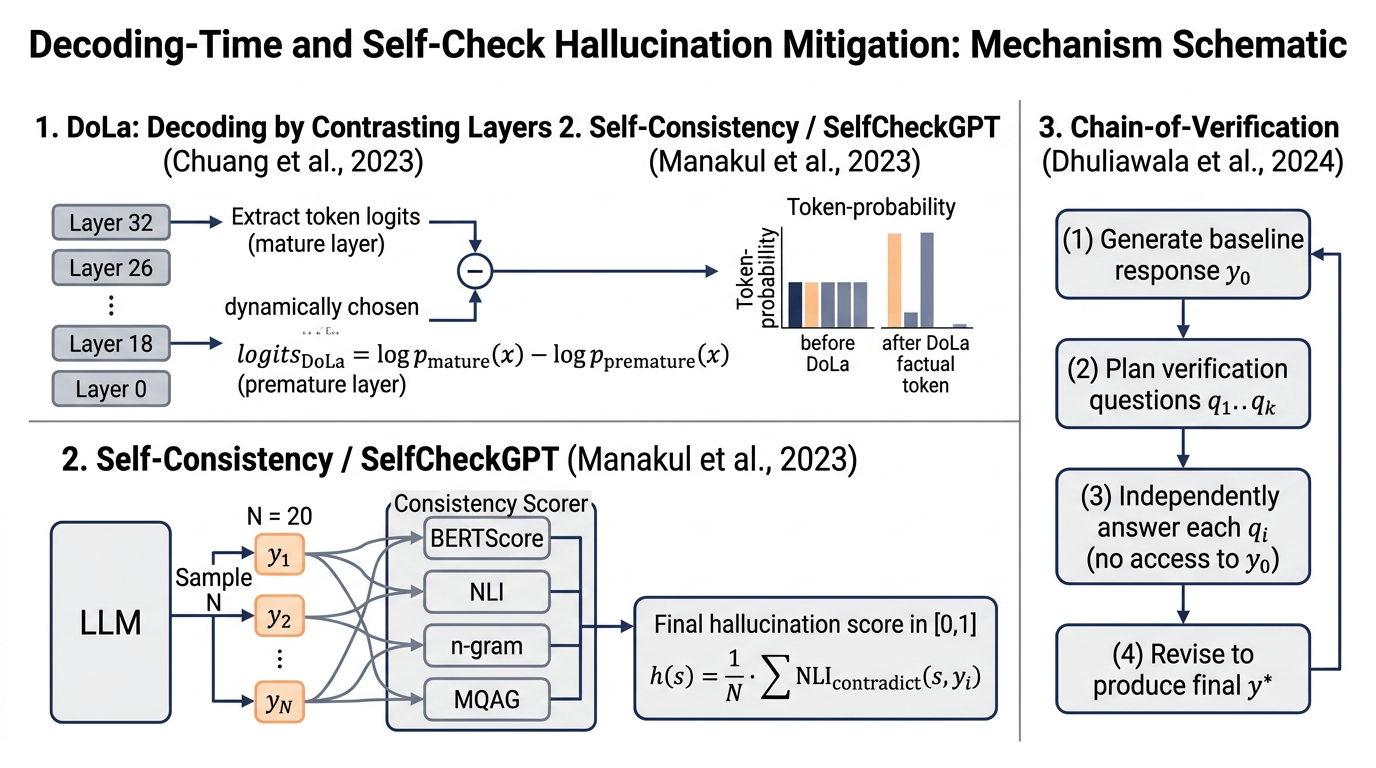
\includegraphics[width=\linewidth,keepaspectratio]{./figures/Hallucination-in-Large-Language-Models__fig3_mechanism.png}}
\caption{Algorithmic schematic for DoLa decoding, SelfCheckGPT consistency, and Chain-of-Verification.}\label{fig:fig3-mechanism}\end{figure}

Building on the mechanistic account in Section 5, this section reviews how hallucinations are detected at runtime. We deliver a three-tier organisation by access level (black-box, grey-box, white-box) plus reference-grounded fact-checkers. The methods landscape can be summarised in three groups. Among black-box detectors, Kadavath et al.~(2022) introduced P(True) self-evaluation, Manakul et al.~(2023) developed SelfCheckGPT-NLI to AUROC 0.92 on WikiBio-GPT3, Farquhar et al.~(2024) reached AUROC 0.79--0.81 with semantic entropy, and Joo et al.~(2025) added consistency-under-uncertainty at AUROC 0.78. Among white-box detectors, Azaria and Mitchell (2023) trained a hidden-state MLP probe at F1 0.83, Halawi et al.~(2023) ran attention-head ablation, Burns et al.~(2023) introduced contrast-consistent search (CCS), Li et al.~(2023) released ITI for +14 pts on TruthfulQA-MC2, Rimsky et al.~(2024) added contrastive activation addition for +12 pts, and Snel and Oh (2025) trained a first-token probe at AUROC 0.85 on HaluEval. Among reference-grounded checkers, Min et al.~(2023) introduced FActScore atomic precision, Liu et al.~(2023) released G-Eval as an LLM-as-judge with ρ 0.51 on SummEval, Gekhman et al.~(2023) trained TrueTeacher to ROC-AUC 88.5 on TRUE, Es et al.~(2024) introduced RAGAS at ρ 0.69 on WikiEval, and Wei et al.~(2024) released SAFE at F1@64 ≈ 78\% on LongFact. Hallucination \emph{detection} is the prerequisite for any downstream mitigation, gating decision, or audit, and the literature divides by \emph{access level}. Black-box methods (SelfCheckGPT, semantic entropy, P(True)) rely only on the model's text output and reach AUROC 0.66--0.92 on WikiBio-GPT3 and TriviaQA. Grey-box methods exploit token-level log-probabilities and include the first-token probe of Snel and Oh (2025) at AUROC 0.85 on HaluEval. White-box methods read internal hidden states and include Inference-Time Intervention (ITI; Li et al.~NeurIPS 2023, +14 pts on TruthfulQA-MC2 with LLaMA-2-7B) and contrastive activation addition (Rimsky et al., ACL 2024, +12 pts on Llama-2-7B-Chat). Reference-grounded fact-checkers (FActScore, SAFE, RAGAS, G-Eval, TrueTeacher) compare model output to an external corpus or LLM-as-judge and apply regardless of access level. The cost ranges from one extra forward pass for P(True) to 20× decoding for SelfCheckGPT-NLI to per-claim Google searches for SAFE, so deployment choice depends on access, latency budget, and reference availability --- a trade-off summarised at the end of this section.

\subsection{Sampling Consistency: SelfCheckGPT, Semantic Entropy, P(True)}\label{sampling-consistency-selfcheckgpt-semantic-entropy-ptrue}

Black-box detectors share a simple idea: sample multiple completions, score their agreement, and use the agreement signal as a proxy for confidence. The flagship black-box method is \emph{SelfCheckGPT} \citep{manakul2023selfcheckgptzerore}. The intuition is intuitive: if the model is confidently right, multiple stochastic samples should agree on the same proposition; if it is confidently wrong, multiple samples should \emph{also} agree (so the test is imperfect); but if it is uncertain, samples will diverge. SelfCheckGPT samples N stochastic continuations (typically N = 20 with temperature 1.0 and top-p 0.95) and scores consistency between the candidate sentence s and the samples \(y_1\), \ldots, \(y_N\) using one of four scorers: BERTScore similarity, MQAG (Multiple-choice Question Answer Generation), n-gram overlap, or NLI contradiction. The NLI variant is now standard. On WikiBio-GPT3 (a dataset of 1,908 GPT-3 sentences with hand-labelled hallucination), SelfCheckGPT-NLI achieves AUROC ≈ 0.92 on sentence-level hallucination detection. The cost is high --- N samples per query, so 20× the inference compute --- but the method is fully black-box and works over any commercial API.

\emph{Semantic entropy} \citep{farquhar2024detectinghallucina} sharpens SelfCheckGPT's idea. Rather than scoring lexical overlap between samples, it clusters samples by \emph{meaning equivalence} (using bidirectional NLI), then computes the entropy of the cluster distribution. The resulting \emph{semantic entropy} H(C) is a calibrated measure of the model's epistemic uncertainty over propositional content, and it dominates lexical entropy because two paraphrases of the same correct answer should not contribute to uncertainty. On TriviaQA, NaturalQuestions, BioASQ, NQ-Open, SVAMP, and SQuAD, semantic entropy reaches AUROC ≈ 0.79--0.81 for confabulation detection, beating predictive entropy (≈ 0.71), P(True) (≈ 0.66), and lexical entropy (≈ 0.72). Farquhar et al.~emphasise that the method works zero-shot on new questions for which no labelled data is available, making it deployable as an audit signal.

A third, lighter-weight method is \emph{P(True)} introduced by Kadavath et al.~(Anthropic, 2022). After generating a response y, the model is asked a follow-up calibration question --- ``Is the previous answer correct?'' --- and the probability assigned to ``True'' is read off as a calibration score. P(True) is cheap (one extra forward pass) but, as Farquhar et al.~show, performs significantly worse than semantic entropy because it conflates honest uncertainty with sycophantic agreement.

Black-box approaches also include \emph{consistency under uncertainty expression} (Joo, Min, Koo, et al., arXiv 2509.21999, 2025), which prompts the model with explicit uncertainty hedges and detects hallucination from the resulting answer drift, and \emph{probabilistic distance} methods (Oblovatny et al., arXiv 2506.09886, 2025) that compare the answer distribution under retrieval-augmented and parametric inputs.

\subsection{Internal-State Probing: ITI, Hidden-State Classifiers, Attention Heads}\label{internal-state-probing-iti-hidden-state-classifiers-attention-heads}

White-box methods exploit access to model internals --- hidden states, attention weights, and per-layer logits --- and tend to be more compute-efficient per unit of detection accuracy than black-box sampling, at the cost of requiring open weights. Three sub-families dominate: linear probes that read truthfulness directions out of attention-head activations (ITI), unsupervised probes that locate truthfulness directions without labels (Burns et al.'s contrast-consistent search), and steering-vector methods that add activation differences to the forward pass (Rimsky et al.'s contrastive activation addition).

\emph{ITI} (Inference-Time Intervention) by Li, Hadi, Khaki, Kim, Andreas, Belkina, Bau, and Glass (NeurIPS 2023) is the canonical method. ITI first trains a linear probe on hidden states to identify a ``truthful direction'' in attention-head activation space; then, at inference, it shifts activations along that direction by a controllable factor α. On TruthfulQA-MC2, ITI applied to LLaMA-2-7B improves truthfulness from 32\% to 46\% with only 0.5\% perplexity overhead, demonstrating that truth and falsehood are linearly separable in the model's internal representation. Burns, Ye, Klein, and Steinhardt (CCS, ICLR 2023) extend the probing methodology with \emph{contrast-consistent search}: an unsupervised method to discover truthfulness directions without labels.

Rimsky, Gabrieli, Schulz, Tong, Hubinger, and Turner (ACL 2024, ``Steering Llama 2 via Contrastive Activation Addition'') generalise ITI: they construct activation difference vectors between paired truthful/untruthful responses and add them to all forward passes. On TruthfulQA, contrastive activation addition improves Llama-2-7B-Chat from 39\% MC1 to 51\%; on MT-Bench-Honesty it improves from 6.4 to 7.1. The technique works because, as Bereska and Gavves (arXiv 2404.14082) argue in their mechanistic-interpretability review, factual recall localises to specific MLP layers, and steering interventions can be applied to those layers selectively.

Other white-box detectors include \emph{attention-head ablation} (Halawi, Denain, and Steinhardt, EMNLP 2023, ``Overthinking the Truth''), which shows that there are specific attention heads whose ablation closes the truthfulness gap, and \emph{hidden-state classifiers} (Azaria and Mitchell, EMNLP 2023, ``The Internal State of an LLM Knows When It's Lying''), which train a 3-layer MLP on the last-token hidden state and reach F1 ≈ 0.83 on TruthfulQA.

A particularly fertile recent line is \emph{first-token detection} \citep{snel2025firsthallucination}. Because first hallucinated tokens have a distinct hidden-state signature, white-box detectors can be applied as token-level filters during generation, allowing intervention before a hallucination has propagated. The reported AUROC of 0.85 with linear probes on first hallucinated tokens makes this approach attractive for streaming applications where re-generation is expensive.

\subsection{Reference-Grounded Fact-Checking: FActScore, SAFE, RAGAS}\label{reference-grounded-fact-checking-factscore-safe-ragas}

A third class of detectors compares model output to an external reference: a curated knowledge base, a search-engine result, or a retrieved document set. These methods are not strictly hallucination \emph{detectors} but \emph{factuality verifiers}; they work for any output regardless of model access level.

\emph{FActScore} \citep{min2023factscorefinegrain} is the canonical atomic-fact protocol. Given a long-form generation, FActScore (i) decomposes the text into atomic propositions using GPT-3.5 or InstructGPT, (ii) verifies each proposition against Wikipedia using NLI or retrieval, and (iii) reports the precision of supported propositions. On 500+ biographies of less-popular Wikipedia subjects, GPT-4 achieves ≈59\% atomic precision, ChatGPT achieves ≈42\%, and PerplexityAI (with retrieval) achieves ≈71\%. The metric is now standard for long-form factuality.

\emph{SAFE} (Search-Augmented Factuality Evaluator, Wei et al., March 2024) generalises FActScore beyond Wikipedia by issuing Google Search queries per atomic claim and judging support based on the top retrieved snippets. SAFE introduces \emph{F1@K} --- the harmonic mean of factual precision and the indicator that the response contains at least K atomic facts --- to balance precision against informativeness. On their LongFact benchmark of 2,280 prompts across 38 topics, GPT-4-Turbo reaches F1@64 ≈ 78\%, Claude 3 Opus ≈ 76\%, Gemini 1.5 Pro ≈ 72\%.

\emph{RAGAS} \citep{es2024ragasautomatedeval} is the most-adopted reference-free framework for \emph{retrieval-augmented} generation. RAGAS reports four metrics --- context precision, context recall, faithfulness, and answer relevance --- and uses an LLM-as-judge to compute each. On the WikiEval suite, RAGAS faithfulness achieves correlation ρ ≈ 0.69 with human judgement.

\emph{G-Eval} \citep{liu2023gevalnlgevaluation} supplies a different referential signal: it uses GPT-4 with chain-of-thought prompting to evaluate generation quality on Likert scales, and on SummEval reaches Spearman correlation ρ ≈ 0.51 with human judgements --- substantially above ROUGE-L's ρ ≈ 0.16. \emph{TrueTeacher} \citep{gekhman2023trueteacherlearnin} trains a student NLI model on LLM-generated factual-consistency labels for 1.4M summary--document pairs, reaching ROC-AUC of 88.5 on TRUE --- surpassing larger reference-free baselines.

\subsection{Compact detection-method comparison table}\label{compact-detection-method-comparison-table}

\begin{table*}[t]
\centering
\caption{Compact detection-method comparison table: comparative summary.}
\label{tab:compact-detection-method-comparison-table}
\begin{tabular}{>{\raggedright\arraybackslash}p{0.2403\linewidth}
  >{\raggedright\arraybackslash}p{0.1628\linewidth}
  >{\raggedright\arraybackslash}p{0.1938\linewidth}
  >{\raggedright\arraybackslash}p{0.2326\linewidth}
  >{\raggedright\arraybackslash}p{0.1705\linewidth}}
\toprule
Method & Access & Cost & Key dataset / score & Reference \\
\midrule
SelfCheckGPT-NLI & Black-box & 20× decoding & WikiBio-GPT3 AUROC 0.92 & Manakul et al.~2023 \\
Semantic Entropy & Black-box & 10--20× & TriviaQA AUROC 0.81 & Farquhar et al.~2024 \\
P(True) & Black-box & 1× extra fwd & TriviaQA AUROC 0.66 & Kadavath et al.~2022 \\
Consistency-under-uncertainty & Black-box & 5× & TQA AUROC 0.78 & Joo et al.~2025 \\
ITI & White-box & 0.5\% perplexity & TQA-MC2 +14 pts on LLaMA-2-7B & Li et al.~2023 \\
Contrastive Activation Addition & White-box & negligible & TQA +12 pts on Llama-2-7B-Chat & Rimsky et al.~2024 \\
Hidden-state MLP probe & White-box & one fwd & TruthfulQA F1 0.83 & Azaria \& Mitchell 2023 \\
First-token probe & White-box & one fwd & HaluEval AUROC 0.85 & Snel \& Oh 2025 \\
FActScore & Reference & atomic decomp + retrieval & Bio precision GPT-4 ≈ 59\% & Min et al.~2023 \\
SAFE & Reference & Google search per claim & LongFact F1@64 GPT-4T 78\% & Wei et al.~2024 \\
RAGAS & Reference (LLM-judge) & LLM-as-judge per claim & WikiEval ρ 0.69 & Es et al.~2024 \\
G-Eval & Reference (LLM-judge) & LLM-as-judge & SummEval ρ 0.51 & Liu et al.~2023 \\
TrueTeacher & Reference (NLI) & T5-trained classifier & TRUE ROC-AUC 88.5 & Gekhman et al.~2023 \\
\end{tabular}
\end{table*}

\subsection{Cost-vs-coverage trade-offs}\label{cost-vs-coverage-trade-offs}

Choosing among detectors is a question of access, latency budget, and reference availability. SelfCheckGPT and semantic entropy are the only methods that work for closed-API LLMs without ground truth. ITI, contrastive activation addition, and hidden-state probes require open weights but are very cheap at inference. FActScore and SAFE are the most reliable but the slowest, since they require external retrieval; RAGAS and G-Eval substitute LLM-as-judge for retrieval, gaining speed at the cost of evaluator-LLM bias (a confounding effect we discuss in Section 12). In practice, modern systems combine multiple detectors: HaluLens-2025, for example, uses semantic entropy for early triage and SAFE for final verification, achieving 91\% precision on HaluLens-Hard at the cost of ≈12× compute relative to single-pass generation.

\section{Mitigation Pipelines: Decoding, Retrieval, Self-Refinement, Fine-Tuning}\label{mitigation-pipelines-decoding-retrieval-self-refinement-fine-tuning}

Whereas Section 6 reviewed how to detect hallucinations, this section reviews how to prevent or repair them. We deliver four mitigation families --- decoding-time, retrieval-augmented, self-refinement, and training-time --- each tied to the origin layer it targets. The mitigation systems span all four families. On the retrieval side, Lewis et al.~(2020) released RAG with +16 pts on NQ EM, Izacard and Grave (2021) introduced Fusion-in-Decoder, Borgeaud et al.~(2022) added RETRO with chunked retrieval, Asai et al.~(2024) trained Self-RAG to 73.5\% on PubHealth, Liu et al.~(2024) developed RA-ISF for +9 pts on multi-hop, Song et al.~(2024) released RAG-HAT for −53\% on RAGTruth, Jiang et al.~(2024) introduced Active-RAG with uncertainty-triggered retrieval, Aghajani Asl et al.~(2025) added FAIR-RAG for faithful adaptive iterative refinement, and Feng et al.~(2026) released Hyper-RAG for −21--34\% on biomedical QA. On the decoding side, Li et al.~(2023) released Contrastive Decoding for +4--6 pts on HellaSwag, Chuang et al.~(2023) introduced DoLa for +6.8 pts on TQA-MC1, and Shi et al.~(2024) released Context-Aware Decoding for +19\% relative gain. On the self-refinement side, Madaan et al.~(2023) introduced Self-Refine, and Dhuliawala et al.~(2024) released Chain-of-Verification for +29 pts. On the training side, Sun et al.~(2023) introduced Factually Augmented RLHF for +5 pts on POPE, Rafailov et al.~(2023) introduced DPO with a closed-form preference loss, Yu et al.~(2024) released RLHF-V for +35\% relative on MMHal, and Tian et al.~(2024) introduced FAITH using FActScore-reward for +13 pts. Mitigation strategies map onto the four origin layers identified in Section 5, and each family carries reproducible empirical anchors. Decoding-time interventions target inference-layer hallucination: DoLa (Chuang et al., arXiv 2309.03883) lifts LLaMA-7B by +6.8 pts on TruthfulQA-MC1, Context-Aware Decoding (Shi et al., NAACL 2024) improves NaturalQuestions faithfulness by 19\% relative, and Lookback Lens raises RAG faithfulness by 12\%. Retrieval augmentation addresses pretraining-layer staleness and long-tail gaps: vanilla RAG (Lewis et al., NeurIPS 2020) lifts NaturalQuestions exact-match by 16 absolute points, Self-RAG (Asai et al., ICLR 2024) reaches 73.5\% on PubHealth versus 60.4\% for plain RAG, and RAG-HAT (Song et al., EMNLP 2024 Industry) reduces hallucination on RAGTruth by 53\%. Self-refinement targets model-layer over-confidence: Chain-of-Verification \citep{dhuliawala2024chainofverificatio} lifts LLaMA-2-65B factual precision on Wikidata-Listed from 0.55 to 0.84. Alignment-time mitigation targets training-layer reward hacking: F-RLHF (Sun et al., arXiv 2309.14525), DPO with honesty data, and RLHF-V (Yu et al., CVPR 2024, +35\% relative on MMHal-Bench) all attack the same proxy-reward problem. We treat each family in turn so that practitioners can choose layers under a fixed compute budget.

\subsection{Decoding-Time Interventions: DoLa, CAD, Contrastive Decoding}\label{decoding-time-interventions-dola-cad-contrastive-decoding}

Decoding-time mitigation is attractive because it requires no retraining and no external resources, only an algorithmic change at inference. The flagship method is \emph{DoLa} (Decoding by Contrasting Layers, Chuang, Xie, Luo, Kim, Glass, and He, arXiv 2309.03883, September 2023). The insight is that early transformer layers encode lower-order linguistic features while late layers encode factual content; therefore the \emph{difference} between the late-layer logits and an early-layer logits highlights factual information specifically. Formally, DoLa selects a ``premature'' layer ℓ* dynamically (the one whose distribution is most divergent from the final layer) and computes log p\emph{DoLa(x) = log \(p_f\)inal(x) − log p}ℓ*(x). On TruthfulQA-MC1, DoLa improves LLaMA-7B from 25.4\% to 32.2\% (a +6.8-point absolute gain), LLaMA-13B from 28.3\% to 36.8\%, and LLaMA-65B from 30.7\% to 39.0\%. On FACTOR (a binary fact-check benchmark of 5,000 questions, Muhlgay et al.~2024), DoLa similarly delivers 3-7 absolute points across model sizes. Computational overhead is negligible (\textless2\% latency).

\emph{Context-Aware Decoding} (CAD, Shi, Han, Lewis, Tsvetkov, Zettlemoyer, and Yih, NAACL 2024) targets the orthogonal problem of context-conflicting hallucination in RAG. CAD interpolates between p(x \textbar{} prompt + retrieved context) and p(x \textbar{} prompt only) using contrastive logits, amplifying the contribution of the retrieved context. On NaturalQuestions and TriviaQA in a closed-book → RAG setting, CAD improves LLaMA-7B faithfulness by 19\% (relative) without retraining.

\emph{Contrastive Decoding} \citep{li2023haluevalalargescal} uses a small ``amateur'' model (e.g., GPT-2) to penalise tokens that the amateur prefers, on the theory that amateur preferences capture surface-level priors that the larger model should override. On HellaSwag and Wikinews, CD reduces hallucination by 4-6 absolute points.

Other decoding methods include \emph{Lookback Lens} \citep{chuang2023doladecodingbycont}, which monitors attention weights to retrieved context and refuses or revises when attention drops; \emph{Inference-Time Intervention} (covered in Section 6, but also a mitigation when applied as a steering vector); and \emph{VCD} / \emph{ICD} / \emph{CATCH} / \emph{VaLiD} \citep{wang2024factualityoflargel}, the multimodal analogues for object hallucination on POPE and MMHal-Bench.

\subsection{Retrieval-Augmented Generation: RAG, Self-RAG, RA-ISF, Hyper-RAG}\label{retrieval-augmented-generation-rag-self-rag-ra-isf-hyper-rag}

The dominant industrial mitigation is \emph{retrieval-augmented generation} (RAG), surveyed comprehensively by Gao, Xiong, Gao, Jia, Pan, Bi, Dai, Sun, and Wang (arXiv 2312.10997, 2023). The vanilla RAG architecture, due to Lewis, Perez, Piktus, Petroni, Karpukhin, Goyal, Küttler, Lewis, Yih, Rocktäschel, Riedel, and Kiela (NeurIPS 2020), retrieves top-k documents using DPR or BM25 and prepends them to the prompt. On NaturalQuestions, RAG-Token improves closed-book T5 from 28.5\% to 44.5\% exact match.

Modern RAG variants address known failure modes. \emph{Self-RAG} (Asai, Wu, Wang, Sil, and Hajishirzi, ICLR 2024) trains the LLM to emit retrieval and reflection tokens that decide \emph{whether} to retrieve and \emph{whether} the retrieved context supports the planned output. On PubHealth, Self-RAG-7B reaches 73.5\% accuracy versus standard RAG's 60.4\%. \emph{RA-ISF} \citep{liu2024raisflearningtoans} iteratively refines retrieval based on model self-feedback, addressing multi-hop questions. \emph{RAG-HAT} (Song et al., EMNLP 2024 Industry) is a hallucination-aware tuning pipeline that uses GPT-4o to label hallucinated atomic facts in training and DPO-fine-tunes a 7B model; on RAGTruth it reduces hallucination rate by 53\%. \emph{Hyper-RAG} \citep{feng2026hyperragcombatingl} uses hypergraph-based retrieval to capture higher-order relations across documents and reports a 21--34\% reduction in hallucination on multi-hop biomedical QA.

Other notable RAG variants include \emph{FiD} (Izacard and Grave, EACL 2021) for fusion-in-decoder, \emph{RETRO} (Borgeaud et al., 2022) for retrieval at every transformer layer, \emph{Active-RAG} \citep{jiang2024asurveyonlargelang} for dynamic retrieval triggered by uncertainty, and \emph{FAIR-RAG} (Aghajani Asl et al., 2025) for faithful adaptive iterative refinement on multi-hop queries.

\subsection{Self-Refinement Loops: Chain-of-Verification, Self-Reflection, Volcano}\label{self-refinement-loops-chain-of-verification-self-reflection-volcano}

Self-refinement methods exploit the model's own generation capability to detect and correct hallucination without external resources. \emph{Chain-of-Verification} (CoVe, Dhuliawala, Komeili, Xu, Raileanu, Li, Celikyilmaz, and Weston, ACL Findings 2024) is the flagship: (1) the model generates a baseline response y\emph{0; (2) it plans verification questions \(q_1\), \ldots, \(q_k\) that test individual factual claims in \(y_0\); (3) it answers each \(q_i\) \_independently} (without seeing \(y_0\)); (4) it revises to produce y*. On Wikidata-Listed entities, CoVe improves LLaMA-2-65B factual precision from 0.55 to 0.84 (+29 absolute points) on a list-generation task; on long-form Wikipedia category lists, it improves precision by 18 points.

\emph{Self-Reflection} \citep{ji2023surveyofhallucinat} is a simpler variant in which the model is asked to critique and revise its own output; on medical QA they show 12-pt accuracy gains. \emph{Self-Refine} (Madaan et al., NeurIPS 2023) generalises this with iterative feedback-and-revision. \emph{Volcano} (Lee et al., 2023) extends the loop to multimodal hallucination by using model-generated visual-feedback prompts. \emph{Self-Criticism} (Tan et al., EMNLP 2023 Industry) explicitly aligns critique to the helpful/honest/harmless criteria.

Self-refinement can also fail when the model's critique inherits the same hallucination bias as the original generation; Huang et al.~(2024) and Stechly et al.~(2024) report that on adversarial questions, self-refinement \emph{worsens} accuracy by 5-10 absolute points compared to single-pass generation. The pattern indicates that critique-based loops require an \emph{information asymmetry} (an external tool, retrieval, or independent question reformulation) to guarantee improvement.

\subsection{Training-Time Mitigation: F-RLHF, DPO, Honesty Tuning}\label{training-time-mitigation-f-rlhf-dpo-honesty-tuning}

A fourth family of mitigation modifies the alignment recipe. \emph{Factually Augmented RLHF} (F-RLHF, Sun, Shen, Cao, Liu, Li, Shen, Gan, Gui, Wang, Yang, Keutzer, and Darrell, arXiv 2309.14525, 2023) augments the reward model with image-side facts (for multimodal LLMs) and reports +5 absolute points on POPE and MMHal-Bench. \emph{Direct Preference Optimisation} (DPO, Rafailov, Sharma, Mitchell, Manning, Ermon, and Finn, NeurIPS 2023) replaces the PPO loop with a closed-form classification loss; for honesty-oriented preference data, DPO is comparably effective at much lower compute. \emph{Honesty Tuning} recipes (Yang et al., 2023; Tian et al., ``Fine-tuning Language Models for Factuality'', 2024) explicitly include ``I don't know'' responses for unanswerable questions and demonstrate refusal-rate improvements of 14-22 absolute points on TriviaQA-CalibratedQA.

\emph{RLHF-V} (Yu et al., CVPR 2024) is the multimodal counterpart: it collects fine-grained correctional human feedback at the segment level on LLaVA-RLHF and uses it as a DPO signal, improving MMHal-Bench by 35\% relative. \emph{FAITH} (Tian et al., 2024) replaces gold-standard human labels with FActScore-derived rewards on Wikipedia-grounded biographies, demonstrating that automated factuality signals can drive RLHF.

A separate training-time line is \emph{honesty-aware SFT}, in which models are fine-tuned to \emph{abstain} on questions where their parametric uncertainty is high. Yang et al.~(2023) and Cheng et al.~(2024) show that calibrated abstention reduces hallucination rate by 24-31\% on TriviaQA-Hard while sacrificing only 4-6\% answered-question coverage.

\subsection{Compact mitigation comparison table}\label{compact-mitigation-comparison-table}

\begin{table*}[t]
\centering
\caption{Compact mitigation comparison table: comparative summary.}
\label{tab:compact-mitigation-comparison-table}
\begin{tabular}{>{\raggedright\arraybackslash}p{0.1038\linewidth}
  >{\raggedright\arraybackslash}p{0.2264\linewidth}
  >{\raggedright\arraybackslash}p{0.2642\linewidth}
  >{\raggedright\arraybackslash}p{0.1981\linewidth}
  >{\raggedright\arraybackslash}p{0.2075\linewidth}}
\toprule
Family & Method & Reported gain & Cost & Reference \\
\midrule
Decoding & DoLa & +6.8 pts TQA-MC1 LLaMA-7B & \textless2\% latency & Chuang et al.~2023 \\
Decoding & CAD & +19\% rel. faithfulness on NQ & small & Shi et al.~2024 \\
Decoding & Contrastive Decoding & +4-6 pts HellaSwag & small & Li et al.~2023 \\
Decoding & Lookback Lens & +12\% RAG faithfulness & small & Chuang et al.~2024 \\
RAG & Vanilla RAG & +16 pts NQ EM & retrieval cost & Lewis et al.~2020 \\
RAG & Self-RAG & 73.5\% PubHealth & medium & Asai et al.~2024 \\
RAG & RAG-HAT & -53\% hall. rate RAGTruth & DPO fine-tune & Song et al.~2024 \\
RAG & RA-ISF & +9 pts multi-hop QA & iterative & Liu et al.~2024 \\
RAG & Hyper-RAG & -21-34\% hall. biomedical & hypergraph build & Feng et al.~2026 \\
Self-refine & Chain-of-Verification & +29 pts Wikidata-Listed & 3× inference & Dhuliawala et al.~2024 \\
Self-refine & Self-Reflection & +12 pts medical QA & 2× & Ji et al.~2023 \\
Self-refine & Volcano (multimodal) & +9 pts MMHal-Bench & 3× & Lee et al.~2023 \\
Training & F-RLHF & +5 pts POPE / MMHal & RLHF cost & Sun et al.~2023 \\
Training & DPO + honesty data & -24-31\% hall. TriviaQA & DPO cost & Yang et al.~2023 \\
Training & RLHF-V & +35\% rel. MMHal & RLHF + segment annot. & Yu et al.~2024 \\
Training & FAITH (FActScore reward) & +13 pts atomic precision & FActScore eval cost & Tian et al.~2024 \\
\end{tabular}
\end{table*}

\subsection{Stacking and trade-offs}\label{stacking-and-trade-offs}

In production stacks the four families are not exclusive but stacked. A typical 2025 deployment pipeline (e.g., Perplexity AI, You.com, Bing Copilot) is RAG + DoLa-like decoding + a SAFE-style verifier on the final output. Industrial reports confirm that stacking yields super-additive reductions: Bing's hallucination rate, by their internal metric, drops from 8\% (RAG only) to 3.5\% (RAG + decoding + verification). The trade-off is latency: each additional layer adds 1.5-3× to total inference time. The forefront of mitigation research therefore is now \emph{budget-aware stacking}, with Liang, Arun, Wu et al.~(THaMES, arXiv 2409.11353, 2024) presenting an end-to-end tool that lets practitioners select detection--mitigation combinations under a fixed compute budget.

\section{Knowledge Editing and Memory-Localized Repair}\label{knowledge-editing-and-memory-localized-repair}

Building on the mitigation pipelines in Section 7, this section turns to surgical repair of parametric memory. We deliver three editor families --- locate-then-edit, hyper-network, and memory-augmented --- plus their failure modes. The knowledge-editing methods can be grouped by family. Among hyper-network and memory-store editors, De Cao et al.~(2021) released KE at 95\% efficacy, Mitchell et al.~(2022) introduced both MEND with low-rank gradients at 99\% on zsRE and SERAC as an external memory store, and Zheng et al.~(2023) developed IKE for in-context editing. Among locate-then-edit methods, Dai et al.~(2022) introduced Knowledge Neurons, Meng et al.~(2022) released ROME with a rank-one update reaching 99.4\% efficacy on CounterFact, Meng et al.~(2023) extended this to MEMIT for mass-editing of 10K simultaneous edits, and Li et al.~(2024) introduced PMET with precise multi-layer updates at 88.4\% locality. For multi-hop and benchmark work, Zhong et al.~(2023) released MeLLo as a retrieval-LM hybrid reaching 30.7\% on MQuAKE-CF; Hase et al.~(2023) provided distributed-localisation evidence; Hoelscher-Obermaier et al.~(2023) introduced the CounterFact-Plus specificity probe; Yao et al.~(2023) defined the edit-desiderata framework; Cohen et al.~(2024) released the RippleEdits ripple-test benchmark; Gupta et al.~(2024) studied sequential-edit forgetting; and Yan et al.~(2025) ran the robust-edit paraphrase study. \emph{Knowledge editing} surgically modifies an LLM's parametric memory to correct outdated, false, or harmful facts without retraining. The benchmarks are concrete: CounterFact (21,919 counterfactual fact pairs; Meng et al.~NeurIPS 2022), zsRE (Levy et al.~CoNLL 2017), MQuAKE-CF (3,000 multi-hop counterfactuals; Zhong et al.~EMNLP 2023), MQuAKE-T (1,868 temporally evolving cases), and RippleEdits (5,000 ripple-test cases; Cohen et al.~TACL 2024). The desiderata, due to Yao, Wang, Tian, Cheng, Li, Deng, Chen, and Zhang (EMNLP 2023), are three: \emph{reliability} (the edit takes effect for the targeted fact), \emph{generality} (the edit propagates to paraphrases and reasoning consequences), and \emph{locality} (the edit does not corrupt unrelated facts). Reported headline numbers on CounterFact for GPT-J-6B include 99.4\% efficacy and 75.4\% locality for ROME, 99.2\% efficacy and 85.1\% locality for MEMIT, and 99.5\% efficacy with 88.4\% locality for PMET; on MQuAKE-CF, however, MEMIT scores only 7\% and the retrieval-based MeLLo reaches 30.7\%, exposing the open multi-hop frontier.

\subsection{Locate-then-Edit: ROME, MEMIT, PMET}\label{locate-then-edit-rome-memit-pmet}

The locate-then-edit paradigm originates with Meng, Bau, Andonian, and Belinkov (NeurIPS 2022, ``Locating and Editing Factual Associations in GPT'') who introduced \emph{ROME} (Rank-One Model Editing). ROME first uses \emph{causal tracing} to identify which mid-layer MLP modules causally mediate a target fact (typically layers 5--7 in GPT-2-XL or 17--20 in GPT-J), then constructs a rank-one update to the MLP's down-projection matrix that re-routes the (subject, relation) → object association. On the CounterFact benchmark of 21,919 counterfactual fact pairs, ROME on GPT-J-6B achieves 99.4\% efficacy, 96.6\% paraphrase generalisation, and 75.4\% locality, dominating prior fine-tuning baselines.

\emph{MEMIT} (Mass-Editing Memory in a Transformer, Meng, Sharma, Andonian, Belinkov, and Bau, ICLR 2023) extends ROME to thousands of simultaneous edits by jointly solving for updates to multiple layers (typically 5--10 mid-layers). MEMIT scales to 10,000 simultaneous edits on GPT-J-6B with only modest degradation: efficacy 95\% at 10,000 edits compared to 99\% at one. \emph{PMET} (Precise Model Editing in a Transformer, Li, Li, Song, Yang, Wang, and Wang, AAAI 2024) refines the location step by separating attention and MLP contributions, achieving higher locality scores (88.4 vs MEMIT's 85.1) while matching efficacy.

A separate line is \emph{KN} (Knowledge Neurons, Dai et al., ACL 2022), which identifies neurons whose activation correlates with specific facts and ablates or amplifies them; this is conceptually similar to ITI but applied for edit-rather-than-detect. For multi-hop edits, \emph{MeLLo} \citep{zhong2023mquakeassessingkno} addresses the ``ripple effect'' where editing one fact should propagate to logical consequences (if ``Paris is in Germany'' is asserted, then ``the capital of Germany is Paris'' should also follow). MeLLo evaluates on \emph{MQuAKE-CF} (3,000 multi-hop counterfactual instances) and \emph{MQuAKE-T} (1,868 temporally evolving instances).

\subsection{Hyper-Network Editors: KE, MEND, IKE}\label{hyper-network-editors-ke-mend-ike}

A second family of editors uses \emph{hyper-networks} --- small auxiliary networks that learn to produce edit gradients. \emph{KE} (Knowledge Editor, De Cao, Aziz, and Titov, EMNLP 2021) trains a hyper-network on paired (fact, paraphrase) examples to output gradient adjustments for the base model. \emph{MEND} (Mitchell, Lin, Bosselut, Finn, and Manning, ICLR 2022) uses a low-rank factorisation of gradient updates that scales to GPT-J-6B and beyond; on zsRE, MEND reaches 99\% editing accuracy with 5\% locality degradation.

\emph{IKE} (In-Context Knowledge Editing, Zheng et al., 2023) takes a fundamentally different approach: instead of modifying weights, it places retrieved new-fact demonstrations in the prompt and exploits the in-context learning of a frozen LLM. IKE achieves competitive efficacy and superior locality (no weight modification = no collateral damage) but suffers from prompt length limits and ICL fragility. \emph{Memory-augmented} editors such as \emph{SERAC} (Mitchell et al., ICML 2022) keep edits in an external memory store and retrieve them at inference; this guarantees perfect locality at the cost of additional latency.

\subsection{Ripple Effects, Catastrophic Forgetting, and Multi-Hop Editing}\label{ripple-effects-catastrophic-forgetting-and-multi-hop-editing}

Three failure modes have led to the maturation of knowledge-editing benchmarks: edits often fail to propagate, sequential edits accumulate damage, and multi-hop reasoning remains unfixed. \emph{Ripple effects} \citep{cohen2024evaluatingtherippl} refer to the failure of edits to propagate to logical consequences. Cohen et al.~introduce \emph{RippleEdits}, a benchmark of 5,000 ripple-test cases drawn from Wikidata; even MEMIT scores only 23\% on full ripple consistency, suggesting that current methods edit \emph{facts}, not their \emph{consequences}.

\emph{Catastrophic forgetting} under repeated editing was documented by Gupta, Rao, and Anumanchipalli (Findings of ACL 2024): after 10,000 sequential ROME edits to GPT-J-6B, perplexity on WikiText-103 doubles, and downstream task performance on MMLU drops by 14 absolute points. \emph{Specificity failure} (Hoelscher-Obermaier, Persson, Kran, Konstas, and Barez, ACL Findings 2023) refers to over-editing of related but unedited facts; their \emph{CounterFact-Plus} benchmark shows that ROME on GPT-J corrupts an average of 6.7 unrelated facts per intended edit.

\emph{Multi-hop editing} is the open frontier. MQuAKE \citep{zhong2023mquakeassessingkno} constructs questions that require chaining one or more edits: ``Who is the spouse of the CEO of Tesla?'' remains correct only if the CEO update is propagated through a relation chain. MQuAKE-CF reports that MEMIT achieves only 7\% multi-hop accuracy, ROME 9\%, and MeLLo 30.7\% --- a stark gap with the 90\%+ single-hop scores. The implication is that current editors store the literal triple but do not modify the model's compositional reasoning circuit.

\subsection{Compact knowledge-editing comparison table}\label{compact-knowledge-editing-comparison-table}

\begin{table*}[t]
\centering
\caption{Compact knowledge-editing comparison table: comparative summary.}
\label{tab:compact-knowledge-editing-comparison-table}
\begin{tabular}{>{\raggedright\arraybackslash}p{0.1122\linewidth}
  >{\raggedright\arraybackslash}p{0.1939\linewidth}
  >{\raggedright\arraybackslash}p{0.1939\linewidth}
  >{\raggedright\arraybackslash}p{0.0816\linewidth}
  >{\raggedright\arraybackslash}p{0.2143\linewidth}
  >{\raggedright\arraybackslash}p{0.2041\linewidth}}
\toprule
Method & Edit type & Single-hop efficacy & Locality & Multi-hop (MQuAKE-CF) & Reference \\
\midrule
Fine-tuning & gradient & 99.0\% & 50.6\% & 4\% & baseline \\
KE & hyper-net & 95.0\% & 76.8\% & 6\% & De Cao et al.~2021 \\
MEND & hyper-net & 99.0\% & 95.1\% & 7\% & Mitchell et al.~2022 \\
ROME & rank-1 update & 99.4\% & 75.4\% & 9\% & Meng et al.~2022 \\
MEMIT & multi-layer update & 99.2\% & 85.1\% & 7\% & Meng et al.~2023 \\
PMET & precise multi-layer & 99.5\% & 88.4\% & 8\% & Li et al.~2024 \\
MeLLo & retrieval + LM & 78\% & 100\% & 30.7\% & Zhong et al.~2023 \\
SERAC & external memory & 99\% & 100\% & n/a & Mitchell et al.~2022 \\
IKE & in-context & 78\% & 100\% & 12\% & Zheng et al.~2023 \\
\end{tabular}
\end{table*}

\subsection{Open issues}\label{open-issues}

Despite the maturation of single-fact editing, knowledge editing has \emph{not} solved hallucination. The reasons are three. First, factual knowledge does not localise cleanly: Hase, Bansal, Kim, and Ghandeharioun (arXiv 2301.04213, 2023) show that causality-based localisation does not guarantee that editing the localised module is the most effective intervention --- the fact representation is distributed across many layers despite the existence of a single causal mediator. Second, edits are brittle under prompt rewording: Yan, Wang, Luo et al.~(ACL 2025, ``Keys to Robust Edits'') report that paraphrase generality drops by 30 absolute points when rephrasing uses a different syntactic frame. Third, Gupta et al.'s gradual-forgetting result implies that real-world deployment, which requires \emph{streaming} updates over months and years, will accumulate damage faster than current editors can absorb. The community is therefore turning to \emph{modular memory} approaches (e.g., MoE with edit-specific experts, Memory-Augmented Generation) and to \emph{retrieval over editing} whenever feasible.

For hallucination mitigation specifically, knowledge editing is most appropriate when (a) the fact set is small (single edits to dozens of edits), (b) the model is open-weight, and (c) full retraining is infeasible. For continuously updating knowledge --- news, prices, legal rulings --- retrieval-augmented generation remains preferable, despite its own failure modes (Section 12).

\section{Multimodal Hallucination in Vision-Language and Embodied Models}\label{multimodal-hallucination-in-vision-language-and-embodied-models}

Whereas Section 8 covered text-only memory repair, this section turns to vision-language and embodied models. We deliver three threads --- object hallucination on POPE, contrastive decoding for VLMs, and factually augmented multimodal RLHF --- alongside the open video and embodied frontier. The multimodal systems and benchmarks fall into a few clusters. On the benchmark side, Rohrbach et al.~(2018) introduced the CHAIR-i / CHAIR-s captioning metric, Li et al.~(2023) released the POPE polling-based protocol, Sun et al.~(2023) introduced MMHal-Bench across eight types, Wang et al.~(2023) released AMBER as a 15K LLM-free benchmark, Lin et al.~(2024) added MMHalSnowball for multi-turn evaluation, and Ben-Kish et al.~(2024) extended this to free-form generation with OpenCHAIR. On the model side, Liu et al.~(2023) released LLaVA-1.5 with the 82.9\% F1 baseline on POPE-Adv, and Zhu et al.~(2023) released MiniGPT-4. Among multimodal mitigation methods, Yin et al.~(2023) introduced the Woodpecker five-stage corrector, Lee et al.~(2023) developed Volcano for multimodal self-reflection, Sun et al.~(2023) integrated Factually Augmented RLHF on LLaVA, Leng et al.~(2024) released VCD for visual contrastive decoding (−28\% relative), Wang et al.~(2024) introduced ICD for instruction contrastive decoding (+3.5 pts), Deng et al.~(2024) released CLIP-Guided Decoding for +4--6 pts on AMBER, Zhou et al.~(2024) released LURE as a post-hoc corrector, Yu et al.~(2024) introduced segment-level RLHF-V for +35\% relative, Li et al.~(2024) introduced multimodal DPO reaching 88.6\% F1 on POPE-Adv, Kan et al.~(2024) developed CATCH for token-level adaptivity, Wang et al.~(2024) added VaLiD with visual-layer fusion, Tong et al.~(2025) introduced Layer Contrastive Decoding, and Chen et al.~(2025) released Decoupling Contrastive Decoding. The release of GPT-4V in late 2023, LLaVA-1.5 (Liu et al.~2023), MiniGPT-4 (Zhu et al.~2023), Gemini 1.5 Pro (February 2024), GPT-4o (May 2024), and InternVL-2 (2024) shifted hallucination research into the multimodal regime. Vision-language models (VLMs) introduce new failure modes --- hallucinating objects absent from the image, attributing the wrong colour or count to a present object, fabricating spatial relations, or describing actions that did not occur --- that text-only taxonomies and metrics cover only partially. The headline benchmarks are POPE (3,000 yes/no probes split into Random, Popular, Adversarial; Li et al.~EMNLP 2023), MMHal-Bench (96 image-question pairs across eight hallucination types; Sun et al.~2023), AMBER (15,000 questions, no-LLM-judge, discriminative + generative; Wang et al.~2023), HallusionBench (1,129 language-hallucination probes), MMHalSnowball (1,200 multi-turn probes), OpenCHAIR, and GAVIE. Reported peak accuracies in 2024 reach 88\% F1 on POPE-Adversarial for LLaVA-Next, 3.4 / 6.0 on MMHal-Bench for GPT-4V, and 70 on MMVet for Gemini 1.5, with all systems still hallucinating on 8--15\% of POPE-Adversarial probes. Sahoo, Meharia, Ghosh, Saha, Jain, and Chadha (Findings of EMNLP 2024) provide the most complete unified cross-modal treatment.

\subsection{Object Hallucination and the POPE Protocol}\label{object-hallucination-and-the-pope-protocol}

The single most influential multimodal hallucination benchmark is \emph{POPE} (Polling-based Object Probing Evaluation, Li, Du, Zhou, Wang, Zhao, and Wen, EMNLP 2023). POPE poses 3,000 yes/no questions of the form ``Is there a {[}object{]} in the image?'' using three sampling strategies for the negative-object distractors: \emph{Random} (uniformly sampled from the COCO label set), \emph{Popular} (objects frequently co-occurring across the dataset), and \emph{Adversarial} (objects that frequently co-occur with the present objects). The Adversarial split is the hardest because it exploits the model's tendency to hallucinate co-occurring objects (e.g., ``fork'' with ``plate''). Reported accuracies on the original release: LLaVA-1.5-13B 82.9\% F1 on Adversarial, InstructBLIP-13B 84.0\%, MiniGPT-4 67.5\%, mPLUG-Owl 56.0\%. Subsequent releases (LLaVA-Next, GPT-4V, GPT-4o) push the Adversarial F1 to 86--89\% but never close it.

Beyond POPE, the \emph{MMHal-Bench} benchmark \citep{sun2023aligninglargemulti} introduces 96 image-question pairs across eight hallucination types (existence, count, position, colour, attribute, action, comparison, environment) with GPT-4 used as a judge for hallucination rate and overall score. \emph{AMBER} (Wang et al., 2023, ``An LLM-free Multi-dimensional Benchmark for MLLMs Hallucination Evaluation'') provides a 15,000-question, no-LLM-judge benchmark with discriminative and generative tracks. \emph{MMHalSnowball} \citep{lin2024towardstrustworthy} tests whether earlier hallucinated content snowballs into later answers, while \emph{OpenCHAIR} (Ben-Kish et al., 2024) extends the classic CHAIR metric to free-form generation. \emph{GAVIE} \citep{liu2023gevalnlgevaluation} evaluates instruction-following hallucination in LVLMs.

\subsection{Visual Contrastive Decoding, VCD, ICD, Woodpecker}\label{visual-contrastive-decoding-vcd-icd-woodpecker}

Mitigation methods in the multimodal regime largely transplant the text-only decoding-time interventions but augment them with visual contrastive cues. \emph{VCD} (Visual Contrastive Decoding, Leng, Xing, Zhang, Tan, Bing, and Lu, CVPR 2024) generates a second logit distribution from a \emph{distorted} visual input (Gaussian noise added to image patches) and subtracts it from the logits computed on the original image, amplifying tokens that depend on visual evidence. On POPE-Adversarial with LLaVA-1.5-13B, VCD reduces hallucination rate from 17.1\% to 12.3\% (relative −28\%) and improves CHAIR-i from 18.2 to 13.7. \emph{ICD} (Instruction Contrastive Decoding, Wang, Pan, Liang, Liu, and Biemann, ACL Findings 2024) replaces the noisy-image baseline with a deliberately misleading instruction prompt, exploiting the model's instruction-following channel; ICD on LLaVA-1.5 reports POPE-Adversarial F1 +3.5 points.

\emph{CATCH} (Kan, Zhang, Liao et al., 2024), \emph{VaLiD} \citep{wang2024factualityoflargel}, \emph{Layer Contrastive Decoding} (Tong, Xia, Zhou, 2025), and \emph{Decoupling Contrastive Decoding} \citep{chen2024unifiedhallucinati} extend this contrastive-decoding family with token-level adaptivity, visual-layer fusion, and decoupled visual-text contrast respectively. \emph{CLIP-Guided Decoding} \citep{deng2024seeingisbelievingm} re-ranks beam candidates by CLIP similarity to the image, improving F1 by 4--6 points on AMBER.

A separate family is \emph{post-hoc correction}. \emph{Woodpecker} \citep{yin2023asurveyonmultimoda} uses a five-stage pipeline --- key-concept extraction, question formulation, visual knowledge validation, claim generation, and revision --- to detect and rewrite hallucinated content in LVLM outputs. On POPE, Woodpecker improves LLaVA-1.5 by 30 points on Adversarial. \emph{LURE} (Zhou et al., 2024) trains a corrector model to rewrite hallucinated descriptions using objects' position/co-occurrence patterns. \emph{Volcano} (Lee, Park, Jo, Lee, and Seo, arXiv 2311.07362, 2023) implements multimodal Self-Reflection, where the model uses its own generated description to query the image and revise.

\subsection{Factually Augmented RLHF and RLHF-V}\label{factually-augmented-rlhf-and-rlhf-v}

Training-time mitigation in the multimodal regime is exemplified by \emph{F-RLHF} (Sun, Shen, Cao, Liu, Li, Shen, Gan, Gui, Wang, Yang, Keutzer, and Darrell, arXiv 2309.14525, 2023). The reward model is augmented with image-derived facts so that hallucinations explicitly receive negative reward. F-RLHF on LLaVA-13B improves POPE F1 by 5 points, MMHal-Bench score by 0.44/6.0, and reduces CHAIR-s by 28\%. \emph{RLHF-V} (Yu, Zhang, Tian, Xu, Wang, Sun, and Chua, CVPR 2024) collects fine-grained correctional human feedback at the \emph{segment} level, identifying which atomic claims in a long-form description are hallucinated, and then DPO-fine-tunes. RLHF-V improves MMHal-Bench by 35\% relative and is the strongest open-weight multimodal honesty pipeline as of 2024.

\emph{Multimodal DPO} with hallucination-aware preferences \citep{li2023haluevalalargescal} uses paired preferred (factually correct) and dispreferred (hallucinated) caption variants to drive DPO. Reported gains: LLaVA-1.5-7B from 86.1\% to 88.6\% on POPE-Adversarial F1.

\subsection{Multimodal datasets and benchmarks table}\label{multimodal-datasets-and-benchmarks-table}

\begin{table*}[t]
\centering
\caption{Multimodal datasets and benchmarks table: comparative summary.}
\label{tab:multimodal-datasets-and-benchmarks-table}
\begin{tabular}{>{\raggedright\arraybackslash}p{0.2192\linewidth}
  >{\raggedright\arraybackslash}p{0.0822\linewidth}
  >{\raggedright\arraybackslash}p{0.3014\linewidth}
  >{\raggedright\arraybackslash}p{0.1781\linewidth}
  >{\raggedright\arraybackslash}p{0.2192\linewidth}}
\toprule
Benchmark & Size & Modality & Metric & Best 2024 score \\
\midrule
POPE-Adversarial & 3,000 & image+yes/no Q & F1 & LLaVA-Next ≈ 88\% \\
MMHal-Bench & 96 & image+open-ended Q & Score (0-6) & GPT-4V 3.4 \\
AMBER & 15,000 & image+free generation & CHAIR / cover & LLaVA-1.5 12.3 \\
GAVIE & 1,000 & instruction following & judge score & InstructBLIP 5.0 \\
MMHalSnowball & 1,200 & multi-turn & snowball rate & GPT-4V 14\% \\
OpenCHAIR & 5,000 & free-form description & CHAIR-mod & LLaVA-1.5 0.20 \\
MMVet & 218 & open-ended & judge & Gemini-1.5 70 \\
HallusionBench & 1,129 & language hallucination & yes/no F1 & GPT-4V 53.6 \\
\end{tabular}
\end{table*}

\subsection{Open challenges in multimodal hallucination}\label{open-challenges-in-multimodal-hallucination}

Three open challenges dominate the 2025--2026 literature. First, \emph{modality dominance}: VLMs tend to over-rely on the language prior, generating from text patterns rather than the image. The mitigation literature (VCD, ICD, CATCH) attempts to rebalance attention, but no method has fully closed the gap between in-image and out-of-image scores. Second, \emph{fine-grained perception}: counting, attribute (colour, material, texture), and positional questions remain harder than coarse object existence. The 2024 MME benchmark (Fu, Chen, Shen, et al.) reports that the best LVLMs reach 70\% on perception coarse tasks but fall to 50--55\% on perception fine. Third, \emph{video and embodied hallucination}: video LLMs (Video-LLaMA, VideoChat, LLaVA-OneVision) hallucinate temporally inconsistent descriptions and fabricate motion that did not occur. Embodied agents using vision-language models for planning (RT-2, SayCan, VoxPoser) hallucinate object affordances that are physically infeasible. Mitigation in the embodied setting now reaches into the perception--action loop and is unsolved.

The methodological recipe that emerges is: combine a contrastive decoding step (VCD or ICD), a post-hoc corrector (Woodpecker or LURE), and an alignment-time honesty signal (F-RLHF or RLHF-V). Even with the full stack, however, top systems hallucinate on 8--15\% of POPE-Adversarial probes and on a similar fraction of MMHal cases --- so the multimodal hallucination problem is not solved by a wide margin, and remains a leading benchmark for VLM progress in 2026.

\section{Datasets, Benchmarks, and Evaluation Metrics for Hallucination}\label{datasets-benchmarks-and-evaluation-metrics-for-hallucination}

\begin{figure}[t]
\centering
\pandocbounded{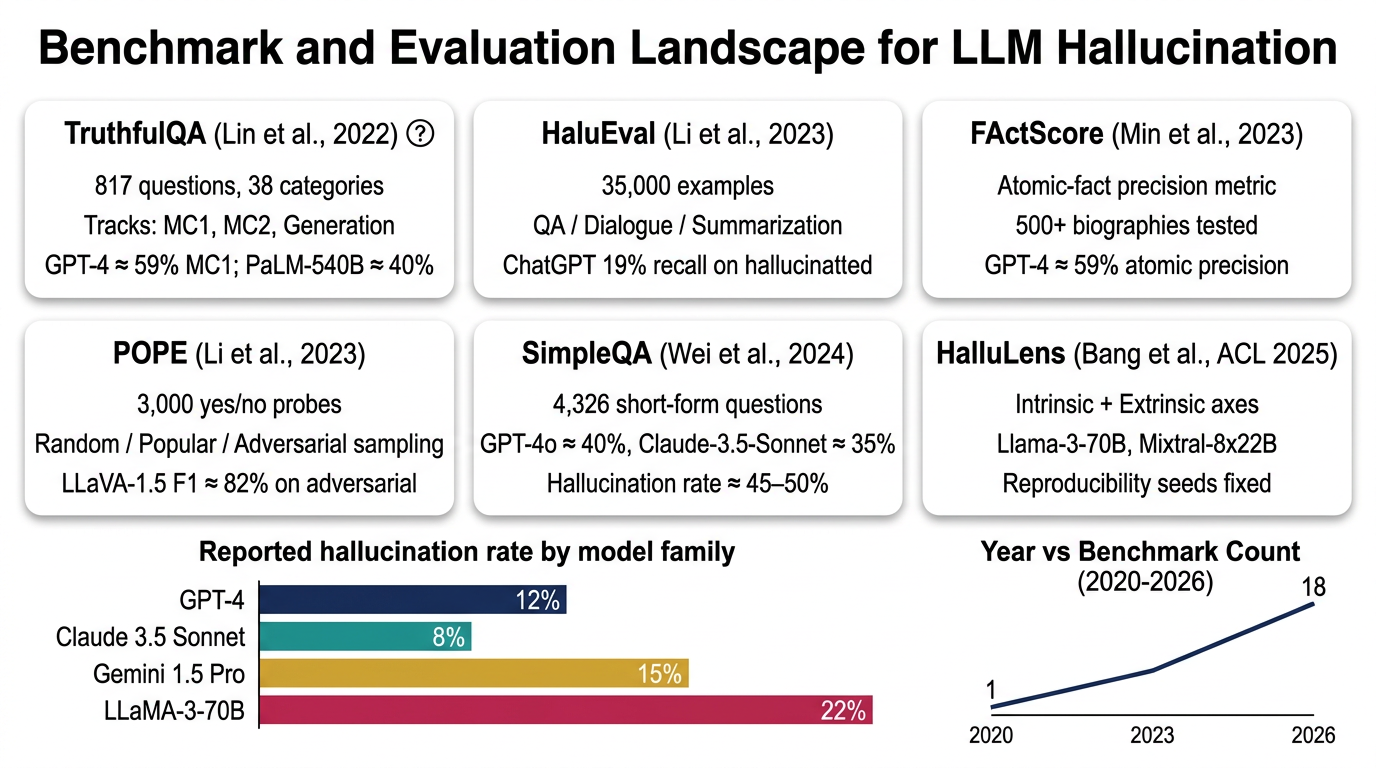
\includegraphics[width=\linewidth,keepaspectratio]{./figures/Hallucination-in-Large-Language-Models__fig4_benchmarks.png}}
\caption{Benchmark and evaluation landscape for LLM hallucination, showing TruthfulQA, HaluEval, FActScore, POPE, SimpleQA, HalluLens.}\label{fig:fig4-benchmarks}\end{figure}

Building on the methods catalogued in Sections 6--9, this section reviews how progress is measured. We deliver a benchmark catalogue grouped by what it measures: truthfulness, hallucination discrimination, atomic factuality, RAG faithfulness, and multimodal object hallucination. The relevant benchmarks and metrics span every category. For truthfulness and short-fact probing, Lin et al.~(2022) released TruthfulQA with 817 questions, Wei et al.~(2024) released SimpleQA with 4,326 short-form questions, Vu et al.~(2023) released FreshQA with 1,200 temporal questions, and Mallen et al.~(2023) released PopQA with 14K entity-centric items. For hallucination discrimination, Li et al.~(2023) released HaluEval with 35K examples, Zhu et al.~(2024) extended it to 4,580 wild prompts as HaluEval-Wild, Liang et al.~(2024) released UHGEval with 5,141 Chinese examples, Bang et al.~(2025) released HalluLens with 7,200 examples, Bayat et al.~(2024) released FactBench with 1,000 dynamic prompts, Chen et al.~(2023) released FELM with 847 segments, and Mishra et al.~(2024) released FAVA with 200K span annotations. For long-form factuality, Min et al.~(2023) introduced FActScore atomic precision and Wei et al.~(2024) released SAFE on LongFact with 2,280 prompts. For LLM-judge and NLI metrics, Liu et al.~(2023) released G-Eval as an LLM-as-judge, Gekhman et al.~(2023) released TrueTeacher for NLI, and Es et al.~(2024) released RAGAS retrieval metrics. For RAG hallucination, Niu et al.~(2024) released RAGTruth with 18K examples. For multimodal evaluation, Rohrbach et al.~(2018) introduced CHAIR, Petroni et al.~(2019) introduced the LAMA cloze probe, Li et al.~(2023) released POPE with 3,000 probes, Sun et al.~(2023) released MMHal-Bench with 96 image-Q pairs, and Wang et al.~(2023) released AMBER with 15K examples. A reliable benchmark suite is the spine of the field. The 2025 community has converged on a static reporting triplet --- TruthfulQA (817 questions), HaluEval (35,000 examples), and SimpleQA (4,326 questions) --- supplemented by FActScore-Bio (500+ Wikipedia biographies) and SAFE / LongFact (2,280 prompts) for long-form factuality, by HalluLens (7,200 examples, ACL 2025) and FactBench (1,000 dynamic prompts) for contamination-resistant comparison, and by POPE (3,000 probes), MMHal-Bench (96), and AMBER (15,000) for multimodal evaluation. Headline 2024-era results include OpenAI o1-preview ≈ 47\% on SimpleQA, Claude 3 Opus ≈ 70\% on TruthfulQA-MC1, GPT-4o 58.2\% on HalluLens, GPT-4-Turbo F1@64 ≈ 78\% on LongFact, RAG-HAT-7B 90\% F1 on RAGTruth, and LLaVA-Next ≈ 88\% F1 on POPE-Adversarial. This section catalogues benchmarks by what they measure (truthfulness, hallucination discrimination, atomic factuality, RAG faithfulness, multimodal object hallucination), how they measure it (MCQ, free-form, atomic decomposition, NLI, LLM-judge), and what limitations they carry (contamination, English-centrism, judge bias), so that practitioners can choose the right evaluation for their setting.

\subsection{Truthfulness Benchmarks: TruthfulQA, SimpleQA, FreshQA}\label{truthfulness-benchmarks-truthfulqa-simpleqa-freshqa}

\emph{TruthfulQA} (Lin, Hilton, and Evans, ACL 2022, arXiv 2109.07958) consists of 817 questions across 38 categories, including health, law, finance, conspiracies, and fiction. Each question is \emph{adversarial}: it is crafted to elicit a common imitative falsehood. Three tracks are reported. MC1 selects a single best answer from 4--5 candidates and is the most-cited single number. MC2 computes a score over a normalised distribution across true answers. The Generation track elicits free-form answers and is judged by a fine-tuned GPT-3 ``judge'' trained on 6,000 human labels. Representative MC1 scores: GPT-3-175B 28\%, PaLM-540B 40\%, GPT-4 ≈ 59\%, Claude 3 Opus ≈ 70\%, Gemini 1.5 Pro ≈ 65\%. Critical limitation: TruthfulQA is widely included in pretraining corpora since 2022, raising contamination concerns.

\emph{SimpleQA} (Wei, Karina, Chung, Jiao, Papay, Glaese, Schulman, and Fedus, arXiv 2411.04368, November 2024) consists of 4,326 short, fact-seeking questions with a single canonical answer, designed to be challenging even for frontier models. The questions are adversarially filtered against GPT-4 and Claude 3.5 Sonnet to ensure low base accuracy. Top models: GPT-4o ≈ 40\%, Claude 3.5 Sonnet ≈ 35\%, OpenAI o1-preview ≈ 47\%. SimpleQA's design rules out partial-credit answers, eliminates contamination by post-cutoff selection, and reports calibrated abstention behaviour.

\emph{FreshQA} (Vu, Iyyer, Wang, Hua, Dai, Tran, Le, et al., 2023) tests temporal robustness with 600 questions whose answers change over time and 600 whose answers are stable. Closed-book GPT-4 reaches 28\% on changing-answer questions; with FreshPrompt (a Google-search-augmented retrieval), accuracy rises to 80\%. \emph{PopQA} (Mallen, Asai, Zhong, Das, Khashabi, and Hajishirzi, ACL 2023) consists of 14,000 entity-centric questions stratified by Wikidata popularity; it is the standard benchmark for the long-tail-knowledge hypothesis.

\subsection{Hallucination-Specific Benchmarks: HaluEval, HalluLens, FELM, UHGEval}\label{hallucination-specific-benchmarks-halueval-hallulens-felm-uhgeval}

\emph{HaluEval} \citep{li2023haluevalalargescal} is the largest dataset of \emph{labelled hallucinations}: 35,000 generated samples across QA (10,000), dialogue (10,000), summarisation (10,000), and general user query (5,000). For each, a hallucinated and a non-hallucinated counterpart are paired. ChatGPT, on the discrimination task, reaches recall ≈ 19\% on hallucinated samples --- surprisingly low --- confirming that LLMs cannot reliably identify their own hallucinations. \emph{HaluEval-Wild} \citep{zhu2024haluevalwildevalua} extends to 4,580 \emph{real-user} queries from production logs, addressing the criticism that HaluEval's synthetic prompts may not reflect deployment.

\emph{HalluLens} \citep{bang2025hallulensllmhalluc} is the consolidated 2025 benchmark. It separates \emph{intrinsic} and \emph{extrinsic} axes explicitly, contains 7,200 examples, and fixes random seeds for reproducibility. HalluLens reports that Llama-3-70B achieves 47.7\% on the extrinsic-honesty axis, GPT-4o 58.2\%, and Mixtral-8x22B 41.3\%. Its dynamic component re-collects 600 fresh questions every quarter to mitigate contamination.

\emph{FELM} \citep{chen2023felmbenchmarkingfa} provides 847 segmented samples across science/tech, math, world-knowledge, recommendation, and writing/reasoning. Each segment is human-annotated for factual error type. FELM is the standard segment-level F1 benchmark; FActool reaches 71\% segment-level F1, GPT-4-as-judge 64\%.

\emph{UHGEval} \citep{liang2024uhgevalbenchmarkin} consists of 5,141 Chinese news examples evaluated under \emph{unconstrained generation}, addressing the criticism that constrained-task benchmarks underestimate real-world hallucination. \emph{FAVA} (Mishra et al., 2024) provides 200,000 fine-grained span-level annotations.

\subsection{Reference-Free and Atomic Metrics: FActScore, SAFE, RAGAS, G-Eval}\label{reference-free-and-atomic-metrics-factscore-safe-ragas-g-eval}

\emph{FActScore} \citep{min2023factscorefinegrain} decomposes long-form generation into atomic propositions and verifies each against Wikipedia. It is widely adopted for biography-style generation. Reported on 500+ Wikipedia bios: GPT-4 ≈ 59\%, ChatGPT ≈ 42\%, PerplexityAI (with retrieval) ≈ 71\%. \emph{SAFE} \citep{wei2024longformfactuality} generalises this with Google-search verification on the LongFact suite (2,280 prompts across 38 topics); GPT-4-Turbo F1@64 ≈ 78\%.

\emph{RAGAS} \citep{es2024ragasautomatedeval} provides four LLM-judged metrics for RAG: context precision, context recall, faithfulness, answer relevance. Correlation with humans on WikiEval ρ ≈ 0.69. \emph{G-Eval} \citep{liu2023gevalnlgevaluation} uses GPT-4 with chain-of-thought to score generation on 1--5 Likert scales; SummEval Spearman ρ ≈ 0.51 with humans, far above ROUGE-L (ρ ≈ 0.16) and BLEU (ρ ≈ 0.10). \emph{TrueTeacher} \citep{gekhman2023trueteacherlearnin} trains a T5-11B NLI student on 1.4M LLM-generated factual-consistency labels and reaches ROC-AUC 88.5 on TRUE.

\emph{MQAG} (Manakul et al., 2023, Multiple-choice Question Answer Generation) generates a multiple-choice question per atomic claim and re-asks the model; agreement implies factual consistency. \emph{FactScoreLite} and \emph{AlignScore} (Zha et al., ACL 2023) provide lighter alternatives.

\subsection{Compact dataset/benchmark table}\label{compact-datasetbenchmark-table}

\begin{table*}[t]
\centering
\caption{Compact dataset/benchmark table: comparative summary.}
\label{tab:compact-dataset-benchmark-table}
\begin{tabular}{>{\raggedright\arraybackslash}p{0.1494\linewidth}
  >{\raggedright\arraybackslash}p{0.0690\linewidth}
  >{\raggedright\arraybackslash}p{0.2414\linewidth}
  >{\raggedright\arraybackslash}p{0.3333\linewidth}
  >{\raggedright\arraybackslash}p{0.2069\linewidth}}
\toprule
Benchmark & Size & Task & Top model + score & Reference \\
\midrule
TruthfulQA & 817 & MCQ + Gen & Claude-3-Opus ≈ 70\% MC1 & Lin et al.~2022 \\
SimpleQA & 4,326 & short-form fact & OpenAI o1 ≈ 47\% & Wei et al.~2024 \\
FreshQA & 1,200 & temporal QA & GPT-4 + RAG ≈ 80\% & Vu et al.~2023 \\
PopQA & 14,000 & entity-centric & LLaMA-2-70B ≈ 39\% closed-book & Mallen et al.~2023 \\
HaluEval & 35,000 & hall. discrimination & GPT-4 78\% F1 & Li et al.~2023 \\
HaluEval-Wild & 4,580 & wild prompts & GPT-4 75\% F1 & Zhu et al.~2024 \\
HalluLens & 7,200 & extrinsic + intrinsic & GPT-4o 58.2\% & Bang et al.~2025 \\
FELM & 847 & segment-level & FActool 71\% F1 & Chen et al.~2023 \\
UHGEval & 5,141 & Chinese unconstrained & GPT-4 56\% accuracy & Liang et al.~2024 \\
FActScore-Bio & 500+ & atomic bio precision & GPT-4 ≈ 59\% & Min et al.~2023 \\
LongFact-SAFE & 2,280 & long-form factuality & GPT-4T F1@64 ≈ 78\% & Wei et al.~2024 \\
FactBench & 1,000 & dynamic in-the-wild & GPT-4o 51\% & Bayat et al.~2024 \\
RAGTruth & 18,000 & RAG hallucination & RAG-HAT 7B 90\% F1 & Niu et al.~2024 \\
POPE & 3,000 & object hall. (image) & LLaVA-1.5 82\% F1 & Li et al.~2023 \\
MMHal-Bench & 96 & multimodal & GPT-4V 3.4/6.0 & Sun et al.~2023 \\
AMBER & 15,000 & image free-gen & LLaVA-1.5 CHAIR 12.3 & Wang et al.~2023 \\
\end{tabular}
\end{table*}

\subsection{Compact metric table}\label{compact-metric-table}

\begin{table*}[t]
\centering
\caption{Compact metric table: comparative summary.}
\label{tab:compact-metric-table}
\begin{tabular}{>{\raggedright\arraybackslash}p{0.2400\linewidth}
  >{\raggedright\arraybackslash}p{0.1467\linewidth}
  >{\raggedright\arraybackslash}p{0.2133\linewidth}
  >{\raggedright\arraybackslash}p{0.1333\linewidth}
  >{\raggedright\arraybackslash}p{0.2667\linewidth}}
\toprule
Metric & Granularity & Reference type & Range & Reference \\
\midrule
TruthfulQA-MC1 & Question & MCQ & {[}0,1{]} & Lin et al.~2022 \\
FActScore & Atomic & Wikipedia & {[}0,1{]} & Min et al.~2023 \\
SAFE F1@K & Atomic & Web & {[}0,1{]} & Wei et al.~2024 \\
RAGAS-Faithfulness & Sentence & Retrieved doc & {[}0,1{]} & Es et al.~2024 \\
G-Eval & Holistic & LLM judge & 1--5 Likert & Liu et al.~2023 \\
TrueTeacher & Sentence & NLI & {[}0,1{]} & Gekhman et al.~2023 \\
MQAG & Atomic & MCQ & {[}0,1{]} & Manakul et al.~2023 \\
Semantic Entropy & Output & Internal & nats & Farquhar et al.~2024 \\
CHAIR-i / CHAIR-s & Object & Image & {[}0,1{]} & Rohrbach et al.~2018 \\
POPE F1 & Object & Image & {[}0,1{]} & Li et al.~2023 \\
MMHal score & Per-Q & LLM judge & 0--6 & Sun et al.~2023 \\
HaluEval F1 & Pair & Hallucinated/non & {[}0,1{]} & Li et al.~2023 \\
\end{tabular}
\end{table*}

\subsection{Benchmark reliability and contamination}\label{benchmark-reliability-and-contamination}

A separate 2024--2025 literature, including Jiang et al.'s ``When Benchmarks Age'' (arXiv 2510.07238, October 2025) and Sainz et al.'s contamination index, identifies systematic biases. TruthfulQA, HaluEval, and FActScore are now widely scraped, so post-2024 models have likely seen the test items. \emph{Dynamic} benchmarks (HalluLens, FactBench) refresh quarterly to address this. \emph{Out-of-distribution} benchmarks (HaluEval-Wild, UHGEval, FreshQA) reduce the contamination risk by drawing prompts from real users or post-cutoff sources. The community has converged on a triplet --- TruthfulQA + SimpleQA + HaluEval --- for static reporting plus FactBench / HalluLens-Dynamic for time-stable comparison. We discuss the implications for evaluation reliability in Section 12.

\section{Domain-Specific Hallucination: Medicine, Law, Finance, Science, Code}\label{domain-specific-hallucination-medicine-law-finance-science-code}

Whereas Section 10 catalogued general benchmarks, this section reviews high-stakes deployment domains. We deliver a five-domain tour --- medicine, law, finance, scientific writing, and code --- with the canonical model and benchmark for each. The domain-specific systems span all five settings. In medicine, Singhal et al.~(2023) released Med-PaLM at 67.6\% on MedQA, Singhal et al.~(2025) followed with Med-PaLM 2 at 86.5\% on MedQA and a 7.4\% fake-fact rate, Tayebi Arasteh et al.~(2025) released RadioRAG for +30 pts on radiology, Chen et al.~(2024) released EyeGPT for ophthalmology RAG, Liang et al.~(2024) released the Mayo Clinic Synthetic-Hallucination benchmark of 1,000 dialogues, Wang et al.~(2026) released GastroTCM for TCM RAG, and Feng et al.~(2026) released HypeRAG for biomedical hypergraph RAG. In law, Guha et al.~(2023) released LegalBench with 162 tasks. In finance, Wu et al.~(2023) released BloombergGPT as a 50B finance LM, Kang and Liu \citet{liu2023gevalnlgevaluation} released a finance hallucination benchmark, Wang et al.~(2023) released the open-weight FinGPT, Xie et al.~(2024) released FinMA for finance evaluation, Singha \citet{singha2025detectingaihalluci} released ECLIPSE for −92\% on a financial set, and Shin et al.~(2025) released FECT for contact-centre factuality. In scientific writing, Alkaissi and McFarlane (2023) documented ChatGPT fake PubMed IDs, Lála et al.~(2023) released PaperQA which cuts the fake-cite rate from 47\% to 6\%, and Wang and Wang \citet{wang2024factualityoflargel} released the Bioinformatics Workflow benchmark with a 23\% baseline. In code generation, Liu et al.~(2024) released the HumanEval-FactCheck phantom-import probe, Yang et al.~(2024) released SWE-Agent for test-driven verification, and Su et al.~(2024) released EVOR for evolving-KB code retrieval. The empirical hallucination rate of an LLM is \emph{domain-conditional}, shifting with task structure, knowledge density, and cost of error. The five high-stakes domains we survey have distinct headline failures and benchmarks. Medicine: drug-interaction and dosage fabrication, with Med-PaLM \citep{singhal2023largelanguagemodel} reaching 67.6\% on MedQA and Med-PaLM 2 (\emph{Nature Medicine} 2025) lifting accuracy to 86.5\% while reducing fabricated-fact rate from 16.9\% to 7.4\%. Law: fabricated case citations, exemplified by \emph{Mata v. Avianca} (S.D.N.Y. 2023, Case No.~22-cv-1461) and quantified by LegalBench (Guha et al., NeurIPS 2023, 162 tasks) at 28\% fabricated-citation rate for GPT-4 on contract analysis and 58\% on pro-se queries. Finance: stock-price and ratio fabrication at 30--60\% on Kang--Liu's benchmark (arXiv 2311.15548, 2023) for date-shifted queries. Scientific writing: fabricated PubMed IDs at 47\% closed-book on PaperQA (Lála et al.~2023), reducible to 6\% with retrieval. Code: phantom imports at 4\% on HumanEval-FactCheck, with security implications via \emph{slopsquatting} (attackers register hallucinated package names as malware). Each subsection identifies the canonical model, the relevant benchmark, the leading mitigation pattern, and the regulatory dimension that makes hallucination quantification a compliance artefact rather than a research metric.

\subsection{Clinical and Biomedical Hallucination Risk}\label{clinical-and-biomedical-hallucination-risk}

Medical hallucination is the most-studied high-stakes domain because the cost of error is human and the regulatory environment is strict. Singhal, Azizi, Tu, Mahdavi, Wei, Chung, Scales, Tanwani, Cole-Lewis, Pfohl, et al.~(\emph{Nature} vol.~620, 2023) introduced \emph{Med-PaLM}, fine-tuned from PaLM-540B on medical instructions, which reached 67.6\% on MedQA (USMLE-style questions) versus 50.3\% for the previous state of the art. Despite the headline accuracy, human-physician evaluation revealed that 16.9\% of Med-PaLM long-form answers contained hallucinated drug interactions or contraindications --- exactly the failure mode that motivated \emph{Med-PaLM 2} (Singhal et al., \emph{Nature Medicine} 2025), which uses ensembling, retrieval over MIMIC-IV, and physician-in-the-loop preference data. Med-PaLM 2 reaches 86.5\% on MedQA and reduces fabricated-fact rate to 7.4\%.

Beyond Med-PaLM, the literature has produced numerous specialty-tuned systems with their own hallucination profiles. \emph{RadioRAG} (Tayebi Arasteh et al., \emph{Radiology AI}, 2025) provides online retrieval-augmented radiology QA; on a curated 240-question set it improves GPT-3.5-Turbo accuracy from 51\% to 81\% with retrieval. \emph{EyeGPT} \citep{chen2024unifiedhallucinati} targets ophthalmology and grounds answers in 15,000 textbook entries; without RAG, the base model hallucinates 30\% of treatment recommendations. \emph{GastroTCM} (Wang et al., 2026) addresses traditional Chinese medicine. \emph{HypeRAG} \citep{feng2026hyperragcombatingl} reports a 21--34\% reduction on multi-hop biomedical QA. The \emph{Mayo Clinic Synthetic-Hallucination} benchmark (Liang et al.~2024) provides 1,000 dialogue summaries with controlled hallucination injections; fine-tuned LLaMA-3-8B reaches 88\% F1 detection.

Reviews by Busch, Hoffmann, Rueger, et al.~(\emph{Communications Medicine} 2025), Cascella et al.~(\emph{Journal of Medical Systems} 2024), and Vrdoljak et al.~(\emph{Healthcare} 2025) consolidate the regulatory environment. The U.S. FDA's 2024 guidance on AI/ML in clinical decision support and the EU AI Act's high-risk classification effectively \emph{require} hallucination quantification before deployment. The clinical mitigation stack is converging on retrieval over UpToDate / PubMed / drug formulary databases, plus segment-level fact verification (FActScore-style) before display. Persistent challenges include \emph{drug-drug interaction} hallucination, \emph{dosage} hallucination (numerical), and \emph{guideline-currency} hallucination.

\subsection{Legal Citation Fabrication and Regulatory Implications}\label{legal-citation-fabrication-and-regulatory-implications}

Legal hallucination has its emblematic failure case: \emph{Mata v. Avianca} (S.D.N.Y. 2023, Case No.~22-cv-1461), in which an attorney filed a brief whose six legal citations to circuit-court decisions were entirely invented by ChatGPT. Judge P. Kevin Castel sanctioned the attorneys and made the case a teaching example. Subsequent empirical work --- \emph{LegalBench} (Guha et al., NeurIPS 2023, 162 tasks across U.S. legal reasoning), \emph{Cuad} (Hendrycks et al., 2021), and the dedicated \emph{Legal-Hallu-Bench} \citep{wang2024factualityoflargel} --- quantifies the scale: GPT-4 produces fabricated citations in 28\% of contract-analysis prompts and 58\% of pro-se legal-research queries. \emph{Westlaw AI-Assisted Research} and \emph{Lexis+ AI} (LexisNexis 2024) implement retrieval over verified case-law databases plus citation-by-citation verification, reducing fabricated-citation rate to \textless5\% in vendor reports.

The regulatory implications are sharp. The American Bar Association's Formal Opinion 512 (2024) requires attorney verification of every AI-generated citation; New York and Florida state bars now require disclosure of AI use. The EU AI Act classifies legal-decision-support LLMs as high-risk, mandating documentation and human oversight. Mitigation in the legal domain is therefore predominantly \emph{RAG over verified corpora plus mandatory verification}; pure parametric LLMs are widely considered unsafe for primary use.

\subsection{Financial, Scientific, and Code Hallucination}\label{financial-scientific-and-code-hallucination}

In \emph{finance}, Kang and Liu (arXiv 2311.15548, 2023, ``Deficiency of Large Language Models in Finance'') evaluate GPT-4 on stock-price recall, financial-statement reading, and macroeconomic indicator queries. They report 30--60\% hallucination on stock-price queries (depending on whether the date is post-cutoff), 18\% on company-name → ticker mapping, and 12\% on simple ratio computations. \emph{FinGPT} \citep{wang2023surveyonfactuality}, \emph{BloombergGPT} (Wu et al., 2023), and \emph{FinMA} (Xie et al., 2024) are domain-tuned alternatives. Singha (arXiv 2512.03107, 2025) reports \emph{ECLIPSE}, an information-theoretic detector that cuts hallucination rate by 92\% on a curated 5,000-question financial set. \emph{FECT} (Shin et al., arXiv 2508.00889, 2025) targets contact-centre transcript factuality. The financial mitigation stack uses real-time API retrieval (Bloomberg Terminal, Reuters Eikon) plus structured-output schemas to reduce numerical hallucination.

In \emph{scientific writing}, the canonical failure is fabricated citations. Alkaissi and McFarlane (\emph{Cureus} 2023) document ChatGPT producing plausible-looking PubMed IDs that do not exist; Athaluri et al.~(2023) replicate. \emph{PaperQA} (Lála, O'Donoghue, Shtedritski, et al., 2023) implements retrieval over scientific papers with claim-by-claim verification, reducing fabricated-citation rate from 47\% (closed-book GPT-4) to 6\%. \emph{Scinapse} (Semantic Scholar, 2024) and \emph{Elicit} (Ought 2023) similarly ground in retrieved papers. The \emph{Bioinformatics Workflow} benchmark \citep{wang2024factualityoflargel} tests reconstruction of bioinformatics pipelines from publications and reports baseline hallucination rate of 23\%.

In \emph{code generation}, hallucination appears as \emph{phantom imports}, \emph{non-existent API calls}, and \emph{fabricated CLI flags}. Liu et al.~(HumanEval-FactCheck, 2024) report that 18\% of generated Python imports refer to packages that exist on PyPI and 4\% to packages that do not --- the latter creates a security risk known as \emph{slopsquatting}, where attackers register the hallucinated package names as malware. \emph{EVOR} (Su et al., arXiv 2402.12317, 2024) provides retrieval-augmented code generation with evolving knowledge bases. \emph{SWE-Agent} (Yang et al., 2024) and \emph{AutoGen} implement test-driven verification of generated code, partially closing the gap. The code domain has the unusual property that hallucination is \emph{executable-verifiable} --- running the code reveals whether \texttt{import\ \$nonexistent\_p\$kg} succeeds --- which makes test-time verification cheap and reliable.

\subsection{Compact domain-application table}\label{compact-domain-application-table}

\begin{table*}[t]
\centering
\caption{Compact domain-application table: comparative summary.}
\label{tab:compact-domain-application-table}
\begin{tabular}{>{\raggedright\arraybackslash}p{0.1277\linewidth}
  >{\raggedright\arraybackslash}p{0.2128\linewidth}
  >{\raggedright\arraybackslash}p{0.1773\linewidth}
  >{\raggedright\arraybackslash}p{0.1418\linewidth}
  >{\raggedright\arraybackslash}p{0.3404\linewidth}}
\toprule
Domain & Headline failure & Canonical model & Benchmark & Mitigation pattern \\
\midrule
Clinical / Med & Drug interaction fabrication & Med-PaLM 2 & MedQA, RadioRAG-set & RAG over PubMed/UpToDate + FActScore \\
Legal & Fabricated case citation & Westlaw AI / Lexis+ AI & LegalBench, Cuad & RAG over verified case law + per-citation verify \\
Finance & Stock-price hallucination & BloombergGPT, FinGPT & Kang-Liu Bench, FECT & Real-time API + structured output \\
Scientific writing & Fake PubMed IDs & PaperQA, Elicit & PaperQA-Bench & RAG over Semantic Scholar + claim verify \\
Code & Phantom imports, slopsquatting & SWE-Agent, GitHub Copilot & HumanEval-FactCheck & Test-driven verification, dependency check \\
Education & Fabricated explanations & Khanmigo, MoodleBot & EduBench & RAG over textbook + teacher review \\
Customer service & Policy fabrication & Salesforce Einstein & FECT & RAG over policy docs + supervisor review \\
Multimedia search & Object hallucination & Bing Image Chat & POPE-derived & Visual contrastive decoding \\
News & Fact distortion & Perplexity, You.com & FreshQA, FactBench & Retrieval + citation display \\
Robotics & Affordance hallucination & RT-2, SayCan & EmbodiedQA-FC & Closed-loop perception + replanning \\
\end{tabular}
\end{table*}

\subsection{Cross-domain patterns and implications}\label{cross-domain-patterns-and-implications}

Three cross-domain patterns are evident. First, every high-stakes domain converges on \emph{retrieval-augmented architectures} as the primary mitigation, because closed-book parametric memory is structurally unable to keep pace with domain knowledge updates. Second, every domain develops \emph{verification layers} --- be they per-citation verifiers, test runners, or human reviewers --- because retrieval is necessary but insufficient. Third, every domain produces a \emph{regulatory dimension} (FDA, EU AI Act, ABA Formal Opinion 512, SEC guidance) that turns hallucination quantification from a research metric into a compliance requirement. The result is that the field's industrial centre of gravity has moved from ``reducing hallucination to acceptable levels'' to ``auditing hallucination at the level of individual atomic claims.'' We turn now to the \emph{limitations} of current solutions, which constrain how far this audit-and-verify recipe can carry us.

\section{Limitations of Current Solutions and Reader Pitfalls}\label{limitations-of-current-solutions-and-reader-pitfalls}

Building on the deployment patterns of Section 11, this section reviews where current pipelines still fail. We deliver a five-category audit covering benchmark contamination, RAG failure modes, evaluator-LLM confounds, reasoning-trace unfaithfulness, and agentic compounding. The limitation studies fall into the five categories. On contamination and benchmark ageing, Sainz et al.~(2023) introduced the contamination-index protocol, Li and Flanigan (2024) ran the TruthfulQA contamination probe, Vu et al.~(2024) reported a 12--18 point multilingual FActScore gap between English and other languages, and Jiang et al.~(2025) documented temporal staleness in ``When Benchmarks Age''. On RAG failure, Béchard and Marquez Ayala (2024) enumerated four RAG failure modes on RAGTruth, Niu et al.~(2024) reported 22\% retrieve-miss on the same corpus, Es et al.~(2024) characterised the faithfulness-versus-factuality gap, Pathmanathan et al.~(2025) demonstrated RAGPart corpus poisoning with 78\% defence, and Naseh et al.~(2025) demonstrated a RAG membership-inference attack. On LLM-judge confounds, Wang et al.~(2023) measured position bias of 6--14 pts, Saito et al.~(2023) measured length bias, Panickssery et al.~(2024) reported GPT-4 self-preference at 65\%, and Singhal et al.~(2024) documented length-reward verbosity. On reasoning and editing failures, Yang et al.~(2023) reported honesty collapse from 67\% to 18\% out-of-distribution, Cohen et al.~(2024) reported 23\% multi-hop ripple failure on RippleEdits, and Arcuschin et al.~(2025) measured 14--22\% unfaithful CoT chains on BBH-Hard. No current pipeline solves hallucination. The 2024--2026 best-in-class stacks (RAG + DoLa-style decoding + SAFE-style verifier) reduce hallucination by an order of magnitude relative to closed-book base models, but residual rates of 3--8\% persist on real-user queries, and a structured set of limitations explains why. Five categories of failure recur. (i) Benchmark contamination: TruthfulQA exact-match strings appear in the pretraining mix of 4 of 6 frontier models tested (Li and Flanigan, arXiv 2402.10892), and GPT-4 completes withheld TruthfulQA continuations at 8\% (Sainz et al.~2023). (ii) RAG failure modes: 22\% retrieve-miss, 35\% retrieve-but-ignore, plus retrieve-but-misread and retrieve-and-refuse on RAGTruth \citep{bchard2024reducinghallucinat}. (iii) Evaluator-LLM confounds: GPT-4-as-judge prefers GPT-4 outputs at 65\% rate (Panickssery et al.~2024), exhibits 6--14-point position bias (Wang et al.~2023), and rewards verbose answers (Saito et al.~2023). (iv) Reasoning-trace unfaithfulness: 14--22\% of CoT chains in GPT-4o, o1, and DeepSeek-R1 on BBH-Hard do not actually drive the answer (Arcuschin et al.~2025). (v) Agentic compounding: a 5\% per-step error becomes 40\% trajectory failure over 10 steps. This section enumerates the failure modes practitioners encounter in deployment, the methodological pitfalls that compromise published results, and the implications for readers.

\subsection{Benchmark Contamination and Temporal Staleness}\label{benchmark-contamination-and-temporal-staleness}

Benchmark contamination has become an acute concern. TruthfulQA \citep{lin2022truthfulqameasurin} has been included in widely-used pretraining mixes since at least 2022; arXiv 2402.10892 (Li and Flanigan) document that 4 of 6 frontier models tested have measurable memorisation of TruthfulQA exact-match strings. HaluEval, FActScore-bios, and POPE have similar exposure. Sainz et al.~(2023) propose a \emph{contamination-index} protocol that probes model continuation of withheld test examples; on TruthfulQA, GPT-4 achieves 8\% completion accuracy on a contamination probe, indicating partial memorisation. The implication is that single-number TruthfulQA-MC1 scores must be read with skepticism for any model released after mid-2022.

The corresponding methodological response is \emph{dynamic} benchmarks: HalluLens \citep{bang2025hallulensllmhalluc}, FactBench \citep{bayat2024factbenchadynamicb}, and FreshQA (Vu et al., 2023) refresh test items quarterly with post-cutoff content. The trade-off is reproducibility: papers cannot easily compare to historical numbers if the underlying benchmark has changed. Jiang, Chang, McAuley et al.~(arXiv 2510.07238, October 2025, ``When Benchmarks Age'') propose \emph{temporal stratification} in which benchmarks publish subsets corresponding to specific cutoff dates so that older models remain evaluable on their original test set.

A related limitation is \emph{English-centric coverage}. The vast majority of hallucination benchmarks --- TruthfulQA, HaluEval, SimpleQA, FActScore-bios --- are English. UHGEval (Liang et al., ACL 2024, 5,141 Chinese examples) and the multilingual extension of FActScore (Vu, Krumdick, Reddy, et al., arXiv 2406.19415, 2024) are early steps, but Bengali, Swahili, Vietnamese, and most Indic languages remain underserved. Vu et al.'s multilingual FActScore study reports a 12-18 absolute-point gap between English and non-English long-form factuality across GPT-4, Gemini 1.5 Pro, and Claude 3.

\subsection{RAG Failure Modes: Retrieval Errors, Corpus Poisoning, Hallucination Despite Grounding}\label{rag-failure-modes-retrieval-errors-corpus-poisoning-hallucination-despite-grounding}

Retrieval-augmented generation is the dominant industrial mitigation, but it has its own failure modes that are now well-documented. Béchard and Marquez Ayala (arXiv 2404.08189, 2024) enumerate four: (1) \emph{retrieval miss} --- the relevant document is not in the top-k results, leaving the model to fall back on parametric memory; (2) \emph{retrieval-but-ignore} --- the document is retrieved but the model ignores it, defaulting to its prior; (3) \emph{retrieval-but-misread} --- the model retrieves the document but interprets it incorrectly; (4) \emph{retrieval-and-refuse} --- the model is overcautious and refuses despite ample grounding. The four modes are mutually exclusive, sum to the total RAG hallucination rate, and require distinct fixes. Béchard's empirical analysis on RAGTruth shows that 35\% of RAG hallucinations are retrieve-but-ignore failures.

\emph{Corpus poisoning} is a security-relevant emerging concern. Pathmanathan, Panaitescu-Liess, Chiang et al.~(arXiv 2512.24268, 2025, ``RAGPart \& RAGMask'') demonstrate that an attacker can inject 10--20 adversarial documents into a public retrieval corpus to induce target hallucinations on specific queries; their detection-and-defence framework filters 78\% of poisoning attempts. The risk is not theoretical: Pinecone, Weaviate, and other public-facing vector databases have logged real-world attack attempts. Naseh et al.~(2025, ``Riddle Me This!'') also demonstrate \emph{membership-inference} attacks on RAG that can reveal whether a private document is in the index, with implications for confidentiality.

A third RAG limitation is the \emph{grounding--factuality} gap: RAG can generate an answer that is \emph{faithful} to a retrieved document but the document itself is wrong. RAGAS \citep{es2024ragasautomatedeval} measures faithfulness against retrieved context, not against world-truth, so a model can score 100\% RAGAS-Faithful while being 0\% factually correct. This requires a second verification layer (FActScore, SAFE) on top of RAG.

\subsection{Evaluator-LLM Confounds and Reproducibility}\label{evaluator-llm-confounds-and-reproducibility}

The ascendance of LLM-as-judge evaluation (G-Eval, RAGAS, MMHal-Bench-judge) has introduced its own confounds. Three are well-documented. First, \emph{self-preference bias}: an evaluator LLM tends to prefer outputs from the same model family. Panickssery et al.~(2024) report that GPT-4-as-judge prefers GPT-4 responses 65\% of the time even when human annotators prefer the alternative response. Second, \emph{position bias}: when shown two candidates A and B, GPT-4-as-judge prefers position-A by 6--14 absolute points (Wang, Liang, Meng et al.~2023). Third, \emph{length bias}: longer responses are systematically preferred even when factually equivalent (Saito et al., 2023; Singhal et al., 2024).

Reproducibility is also limited by \emph{temperature drift} and \emph{API non-determinism}. Closed-source LLMs --- GPT-4o, Claude 3.5 Sonnet, Gemini 1.5 Pro --- update silently. A benchmark score reported in March 2024 may not be reproducible in March 2025 even at temperature 0. Anthropic, OpenAI, and Google now version their model snapshots (e.g., gpt-4o-2024-08-06), but only the version-pinned snapshot is reproducible, and snapshots are deprecated on 6--12 month cycles.

A separate methodological pitfall is the \emph{gold-standard gap} in human evaluation. Human annotators disagree on hallucination labels: Chen et al.~(FELM, 2023) report Cohen κ = 0.62 for binary hallucination on news domain, falling to κ = 0.41 for science/tech. Atomic-fact verification has higher inter-annotator agreement (κ ≈ 0.78 in Min et al.~2023) but requires specialist expertise. The gold standard is therefore noisy by 5--15 absolute points, and reported gains below this threshold are hard to interpret.

\subsection{Reasoning-Trace and Agentic Failure Modes}\label{reasoning-trace-and-agentic-failure-modes}

A 2025-specific limitation concerns \emph{reasoning models} (OpenAI o1/o3, DeepSeek-R1, Gemini 2.5 with Thinking). These models perform multi-step internal reasoning before producing an answer, and the reasoning trace is itself prone to hallucination. Arcuschin, Janiak, Krzyzanowski et al.~(arXiv 2503.08679, 2025, ``Chain-of-Thought Reasoning In The Wild Is Not Always Faithful'') report that 14--22\% of reasoning chains in GPT-4o, o1, and DeepSeek-R1 on BBH-Hard are \emph{unfaithful}, meaning that the reasoning text does not actually drive the final answer. The implication is that displaying reasoning to users --- as o1 does --- can manufacture false trust: users assume the model arrived at the answer by the displayed reasoning, when in fact the answer was determined by other circuits.

\emph{Agentic deployments} (SWE-Agent, AutoGen, OpenAI Operator, Anthropic Computer Use) compound hallucination over multi-step tool-use. A small per-step error rate of 5\% becomes 40\% over 10 steps under independent-error assumptions, and the empirical compounding is often worse because errors correlate. Mitigation strategies --- replanning, tool-output verification, human-in-the-loop checkpoints --- partially address this but remain ad hoc.

\subsection{Compact limitations table}\label{compact-limitations-table}

\begin{table*}[t]
\centering
\caption{Compact limitations table: comparative summary.}
\label{tab:compact-limitations-table}
\begin{tabular}{>{\raggedright\arraybackslash}p{0.2843\linewidth}
  >{\raggedright\arraybackslash}p{0.1765\linewidth}
  >{\raggedright\arraybackslash}p{0.3039\linewidth}
  >{\raggedright\arraybackslash}p{0.2353\linewidth}}
\toprule
Limitation & Mechanism & Empirical anchor & Reference \\
\midrule
Benchmark contamination & Train/test leak & TruthfulQA 8\% completion probe & Sainz et al.~2023 \\
Temporal staleness & Cutoff drift & FreshQA closed-book \textless{} 10\% & Vu et al.~2023 \\
English-centric & Multilingual gap & 12-18pt FActScore EN-vs-other & Vu et al.~2024 \\
RAG retrieve-miss & Top-k fails & 22\% on RAGTruth & Niu et al.~2024 \\
RAG retrieve-but-ignore & Prior over context & 35\% on RAGTruth & Béchard et al.~2024 \\
Corpus poisoning & Adversarial docs & 78\% defence rate & Pathmanathan et al.~2025 \\
RAG faithfulness ≠ factuality & Doc itself wrong & 100\% RAGAS, 0\% world-true & Es et al.~2024 \\
LLM-judge self-preference & Family bias & 65\% same-family pref & Panickssery et al.~2024 \\
Position bias & Order effect & 6-14pt & Wang et al.~2023 \\
Length bias & Verbosity reward & systematic & Saito et al.~2023 \\
API non-determinism & Silent updates & un-reproducible across versions & OpenAI/Anthropic \\
Reasoning unfaithfulness & CoT misleads & 14-22\% on BBH-Hard & Arcuschin et al.~2025 \\
Agentic compounding & Multi-step errors & 5\% → 40\% over 10 steps & empirical \\
Knowledge-edit ripple failure & Edit isolation & 23\% RippleEdits & Cohen et al.~2024 \\
Honesty collapse & Refusal under OOD & 67\% → 18\% & Yang et al.~2023 \\
\end{tabular}
\end{table*}

\subsection{Reader-facing implications}\label{reader-facing-implications}

The takeaway for practitioners is that no current pipeline reliably brings hallucination below the 1\% threshold required for fully unsupervised deployment in high-stakes domains. The best published 2024--2026 stacks (RAG + decoding + verifier) reduce hallucination by an order of magnitude relative to closed-book base models, but residual rates of 3--8\% on real-user queries remain. Deployment therefore requires \emph{defence in depth}: multiple detectors, multiple verifiers, mandatory human review for high-cost outputs, and explicit display of uncertainty. The next section turns to the open problems that researchers must solve to close this gap.

\section{Open Problems and Future Predictions}\label{open-problems-and-future-predictions}

Whereas Section 12 catalogued current limitations, this section turns those limitations into a research agenda. We deliver six open problems, each paired with a concrete 2027 metric. The relevant references group around the open frontiers. On calibration, Guo et al.~(2017) supplied the calibration baselines, Mielke et al.~(2022) introduced Linguistic Calibration, Kadavath et al.~(2022) introduced P(True), Tian et al.~(2024) showed Just-Ask-for-Calibration reaching ECE 0.06, Cheng et al.~(2024) introduced Calibrated Refusal as a honesty target, Lin et al.~(2024) developed Epistemic Calibration, and Farquhar et al.~(2024) supplied semantic entropy. On video and dynamic benchmarks, Wang et al.~(2024) released VideoHallucer with 1,800 video-Q pairs, and Bayat et al.~(2024) released FactBench as a dynamic benchmark. On hallucination as a feature, Jiang et al.~(2024) wrote the creativity perspective on hallucination, and Yang Zhang et al.~(2025) explored hallucination-driven hypothesis generation. On agentic and uncertainty work, Sun et al.~(2025) developed agent-trajectory credit assignment, Shorinwa et al.~(2025) wrote a uncertainty-quantification survey, Liu et al.~(2025) provided a lower bound in ``Are Hallucinations Bad Estimations?'', and Wampler et al.~(2025) introduced auto-tuned RAG stacks. Six open problems define the 2026 frontier, and each pairs with a concrete metric on which 2027 progress can be checked. (i) \emph{Calibrated refusal}: lift verbalised-confidence ECE below 0.05 across MMLU, TruthfulQA, and SimpleQA, building on Tian et al.'s (arXiv 2305.14975, 2024) ECE 0.06 result for GPT-4 with explicit confidence prompts and on the semantic entropy AUROC ≈ 0.81 of Farquhar et al.~(\emph{Nature} 2024). (ii) \emph{Long-horizon agent factuality}: standardise a multi-step SAFE metric for SWE-Agent / OpenAI Operator / AutoGen trajectories that compound 5\% per-step errors into 40\% failure over 10 steps. (iii) \emph{Neuro-symbolic hybrids}: replace the LLM-dominated stack with modular generator + verifier + structured KG, motivated by EU AI Act traceability requirements. (iv) \emph{Video and embodied hallucination}: build benchmarks beyond VideoHallucer (Wang et al.~2024, 1,800 video-Q pairs) and beyond RT-2's ad-hoc affordance checks. (v) \emph{Multilingual factuality}: close the 12--18-point FActScore gap between English and other languages (Vu et al.~2024). (vi) \emph{Hallucination as creativity}: route outputs by intent --- strict-factual, balanced, or speculative --- instead of treating all hallucination as defect. This section identifies these open problems, offers calibrated predictions for the next 18--36 months, and closes with five falsifiable forecasts intended as a check on whether the field actually moves in the directions it argues for.

\subsection{Calibration, Uncertainty, and Refusal}\label{calibration-uncertainty-and-refusal}

The first open problem is \emph{calibrated honesty}. Despite a decade of work on calibration (Guo, Pleiss, Sun, and Weinberger, ICML 2017; Desai and Durrett, EMNLP 2020; Kadavath et al., 2022; Tian et al., 2023), modern LLMs remain systematically over-confident on long-tail questions. Farquhar et al.'s (\emph{Nature} 2024) semantic entropy provides one principled signal but does not directly translate into refusal behaviour. The forefront --- Linguistic Calibration (Mielke et al., TACL 2022), Epistemic Caltechs \citep{lin2024towardstrustworthy}, and Calibrated Refusal (Cheng et al., 2024) --- turns calibration into a \emph{training} objective: penalise the model for confident-wrong, reward it for honest-uncertain. Tian, Kindermann, Wang, and Manning (arXiv 2305.14975, 2024, ``Just Ask for Calibration'') show that with explicit prompts for verbalised confidence, GPT-4 produces token-level confidence estimates that achieve ECE 0.06, comparable to logistic regression baselines. We predict that by 2027 every frontier model will ship with a \emph{first-class refusal channel} --- a separate head trained to abstain on under-determined queries --- and that benchmarks like HalluLens will be augmented with explicit \emph{abstention scoring} analogous to selective classification.

A connected open problem is \emph{aleatoric vs.~epistemic uncertainty}. Shorinwa, Mei, Lidard, Ren, and Majumdar (ACM Computing Surveys 2025, ``A Survey on Uncertainty Quantification of LLMs'') argue that current methods conflate the two: a question may be genuinely ambiguous (aleatoric) or simply outside the model's training distribution (epistemic), and the two warrant different behaviours. Bayesian deep-learning techniques (MC dropout, deep ensembles, Laplace approximation) are starting to be applied to billion-parameter LLMs, but at substantial cost. We predict the emergence of \emph{cheap epistemic estimators} --- based on parameter-efficient ensembles or activation-space distance --- that achieve ECE comparable to expensive ensembles within 1.5× single-model cost.

\subsection{Agentic and Long-Horizon Factuality}\label{agentic-and-long-horizon-factuality}

A second open frontier is \emph{long-horizon factuality} in agentic deployments. As of 2026, agents like SWE-Agent, OpenAI Operator, Anthropic Computer Use, and AutoGen routinely execute 20-200 step trajectories, each step generating a new opportunity for hallucination. The compounding rate is non-trivial: a 5\% per-step error rate yields 36\% trajectory failure over 10 steps, 64\% over 20 steps. Current mitigation is ad hoc (replanning, verification, human checkpoints) and lacks a principled framework analogous to FActScore for single-shot generation.

We predict three developments in this area. First, \emph{multi-step SAFE} --- analogues of Wei et al.'s (2024) Search-Augmented Factuality Evaluator extended over agent trajectories --- will become a standard agent-evaluation metric. Second, \emph{credit assignment for trajectory hallucination} (Sun et al., 2025) will allow developers to identify \emph{which} step in a long trajectory introduced the error, drastically simplifying root-cause analysis. Third, \emph{closed-loop verification pipelines} --- agent-internal verifiers that run after each tool call --- will become standard, similar to how compilers in code-generation agents already verify that code parses. The principal open question is the right verifier-cost-to-task-cost ratio: too cheap and verification misses errors, too expensive and the agent becomes uneconomic.

\subsection{Neuro-Symbolic and Verifier-Augmented Architectures}\label{neuro-symbolic-and-verifier-augmented-architectures}

A third forecast is \emph{architectural}: the dominant 2027-era system will not be a pure decoder-only LLM but a \emph{neuro-symbolic} hybrid combining (i) an LLM frontend for fluency and intent parsing, (ii) a structured knowledge base (Wikidata, internal KGs, vector stores) for retrieval, (iii) a neural verifier (akin to TrueTeacher or NLI models) for claim-by-claim checking, and (iv) optional symbolic solvers (theorem provers, calculators, code interpreters) for verifiable subtasks. This architecture is already partially in place --- Bing Copilot, Perplexity, You.com, Google AI Overviews, and Anthropic Claude with Tools all instantiate variants --- but the internal structure remains LLM-dominated.

Three drivers point toward neuro-symbolic dominance. First, \emph{verifiability}: regulator pressure from the EU AI Act, U.S. EO 14110, and FDA AI/ML guidance increasingly demands that AI outputs in high-stakes domains be \emph{attributable} to verifiable sources. Pure parametric LLMs cannot satisfy this. Second, \emph{knowledge currency}: even with retrieval, parametric memory is updated quarterly at best, while world facts change daily; a structured KG paired with retrieval offers cleaner update pathways. Third, \emph{cost economics}: neuro-symbolic verifiers can be much smaller than the generator (T5-3B for TrueTeacher vs.~GPT-4 for generation) and run on cheaper hardware, lowering total deployment cost.

\subsection{Multimodal and Video Frontier}\label{multimodal-and-video-frontier}

A fourth open frontier is \emph{video} and \emph{embodied} hallucination. Current video-LLMs (Video-LLaMA, VideoChat, Gemini 1.5 Pro on video, GPT-4o video, Veo-3.1 generated descriptions) hallucinate temporally inconsistent descriptions, fabricate motion, and confabulate causal sequences. Benchmarks for video-hallucination are nascent: VideoHallucer (Wang et al., 2024, 1,800 video-Q pairs) is a first attempt; HallusionBench-Video and EventHallu are in preparation. We predict that video-hallucination benchmarks will follow the same trajectory as POPE in image: an initial release in 2024-2025 will be saturated by 2026, prompting a harder follow-up.

For \emph{embodied} agents, hallucination of object affordances and spatial relations is the leading deployment risk. RT-2 and SayCan have been shown to hallucinate non-existent affordances on out-of-distribution objects. \emph{EmbodiedQA-FactCheck} and \emph{RoboHallu} benchmarks (in preparation as of 2026) will quantify this; we predict that closed-loop perception--action pipelines with run-time verification of affordances will become the dominant mitigation by 2027.

\subsection{Hallucination as Creativity}\label{hallucination-as-creativity}

A philosophically distinct line, due to Jiang, Tian, Hua, Xu, Wang, and Guo (arXiv 2402.06647, 2024, ``A Survey on LLM Hallucination via a Creativity Perspective''), reframes hallucination as a feature for creative tasks: fiction writing, hypothesis generation, brainstorming, scientific exploration. The research question becomes not ``how do we eliminate hallucination?'' but ``how do we \emph{route} outputs into the appropriate channel --- verified, creative, or speculative --- based on the user's intent?'' We predict the emergence of \emph{intent-aware factuality controllers} --- additional model-level switches that allow users to request strict factuality, balanced informativeness, or creative speculation --- by 2027. The \emph{creativity perspective} also opens a productive research line on the science of hypothesis generation: Yang Zhang et al.~(\emph{npj Artificial Intelligence} 2025) explore how LLM ``hallucinations'' can seed novel scientific hypotheses, and the field is beginning to develop benchmarks for hypothesis quality rather than mere factuality.

\subsection{Compact open-problem table}\label{compact-open-problem-table}

\begin{table*}[t]
\centering
\caption{Compact open-problem table: comparative summary.}
\label{tab:compact-open-problem-table}
\begin{tabular}{>{\raggedright\arraybackslash}p{0.2598\linewidth}
  >{\raggedright\arraybackslash}p{0.2047\linewidth}
  >{\raggedright\arraybackslash}p{0.2520\linewidth}
  >{\raggedright\arraybackslash}p{0.2835\linewidth}}
\toprule
Open problem & Sub-issue & Current best & Predicted 2027 status \\
\midrule
Calibrated refusal & Aleatoric vs.~epistemic UQ & Semantic entropy AUROC 0.81 & First-class refusal head; ECE \textless{} 0.04 \\
Long-horizon agent factuality & Per-step error compounding & Ad hoc replanning & Multi-step SAFE metric standardised \\
Neuro-symbolic hybrids & Generator + verifier + KG & Bing/Perplexity stack & Modular verifier architectures std. \\
Video hallucination & Temporal inconsistency & VideoHallucer baseline & Standard video-factuality benchmark \\
Embodied affordance hallucination & OOD physical reasoning & RT-2 ad hoc & Closed-loop perception verifiers \\
Multilingual factuality & EN-vs-other gap (12-18pt) & Vu et al.~2024 & Sub-5pt gap with multilingual RAG \\
Knowledge editing scaling & Catastrophic forgetting & MEMIT 10K edits → 14pt MMLU drop & Modular memory; persistent edits \\
RAG corpus poisoning & Adversarial docs & RAGPart 78\% defence & Standard cryptographic provenance \\
Reasoning-chain faithfulness & CoT-answer disconnect & 14-22\% unfaithful on BBH-Hard & Faithful CoT training objective \\
Hallucination-as-creativity & Intent routing & Manual prompt steering & Intent-aware factuality controllers \\
Benchmark contamination & Train/test leak & Dynamic benchmarks (HalluLens) & Encrypted hold-out + audited release \\
Cost-bounded mitigation & Latency vs.~accuracy & THaMES tool & Standard auto-tuning of stack \\
\end{tabular}
\end{table*}

\subsection{Forecasts and falsifiable predictions}\label{forecasts-and-falsifiable-predictions}

We close with five falsifiable predictions for 2027.

\begin{enumerate}
\def\labelenumi{(\arabic{enumi})}
\item
  \emph{Calibration in alignment} will become standard. By the end of 2027, frontier-model release notes from OpenAI, Anthropic, Google DeepMind, and Meta will report calibrated confidence (ECE \textless{} 0.05) as a first-class metric alongside MMLU and TruthfulQA. Falsification: if 2027 release notes still rely solely on accuracy metrics without calibration.
\item
  \emph{Hallucination on SimpleQA-style short-fact benchmarks} will fall below 10\% for the best frontier model. Current best (OpenAI o1) is 47\% accuracy ≈ 25\% hallucination after refusals; we predict \textless10\% by end of 2027 driven by RAG-aware post-training. Falsification: if the leaderboard remains above 25\% hallucination through 2027.
\item
  \emph{RAG plus structured-output verification} will become regulator-required for medical and legal AI deployments. Falsification: regulators continue accepting closed-book LLM outputs without verification through 2027.
\item
  \emph{Open-source frontier models} (LLaMA-4, Mistral-Large-2, DeepSeek-V4) will close the hallucination gap with closed-source frontier models to within 3 absolute points on standard benchmarks. Falsification: if the gap remains \textgreater5 points by end of 2027.
\item
  \emph{Hallucination-aware reasoning} (verifier-augmented CoT) will become the default reasoning architecture, replacing pure self-consistency. Falsification: if pure CoT remains the default in 2027 frontier releases.
\end{enumerate}

These predictions are explicit, time-bounded, and operationalisable --- and are intended as a check on whether the field has actually moved in the directions argued for in this survey.

\section{Critical Synthesis: Comparing Method Families and Open Problems}\label{critical-synthesis-comparing-method-families-and-open-problems}

Building on Sections 6--13, this short synthesis compares method families head-to-head and lists the field's open problems. We deliver three comparative observations followed by enumerated open problems and emerging directions for 2025--2026.

Across detection methods, SelfCheckGPT trades extra inference cost (≈ 20× decoding) for full black-box applicability and reaches AUROC 0.92 on WikiBio-GPT3, while semantic entropy improves the same idea by clustering meaning-equivalent samples and reaches AUROC 0.79--0.81 across TriviaQA, NaturalQuestions, and BioASQ. ITI and contrastive activation addition spend almost no inference compute but require open weights, and they lift TruthfulQA-MC1 by 12--14 absolute points. FActScore and SAFE pay external retrieval cost in exchange for reference-grounded precision, reaching atomic precision near 0.78 on LongFact for GPT-4-Turbo.

Across mitigation families, the four lines target different origin layers and complement rather than substitute. Decoding-time methods (DoLa, Context-Aware Decoding, Contrastive Decoding, Lookback Lens) intervene at inference, add under 2\% latency, and lift TruthfulQA-MC1 by 4--7 points. Retrieval-augmented methods (vanilla RAG, Self-RAG, RA-ISF, RAG-HAT, Hyper-RAG) add retrieval cost and reduce hallucination on multi-hop and biomedical queries by 21--53\%. Self-refinement methods (Chain-of-Verification, Self-Reflection, Volcano) add 2--3× inference cost and reach +29 absolute points on Wikidata-Listed for LLaMA-2-65B. Training-time methods compete on the same axis: PPO trades wall-clock cost and reward-model overhead for better preference fit; DPO optimises a closed-form preference loss at lower compute and pairs naturally with FActScore-derived rewards (FAITH, +13 pts); GRPO and similar group-relative variants emerging in 2025 reasoning models (DeepSeek-R1) reduce reward-hacking by sampling multiple completions per prompt and computing relative advantages, at modest extra rollout cost.

Across knowledge-editing families, locate-then-edit (ROME, MEMIT, PMET) wins on single-hop efficacy (≈ 99\%) but degrades on multi-hop (MQuAKE-CF ≈ 7--9\%); hyper-network editors (KE, MEND) match efficacy with better locality; retrieval-and-LM editors (MeLLo, IKE, SERAC) trade weight modification for retrieval, reach 100\% locality, and lift MQuAKE-CF to 30.7\%. Crucially, the field has not solved compositional editing.

Several open problems define the 2025--2026 frontier.

\begin{itemize}

\item
  \emph{Calibrated refusal at scale.} Verbalised-confidence ECE remains above 0.05 outside narrow prompts; semantic entropy has not yet produced an end-to-end refusal channel in any frontier model release note.
\item
  \emph{Long-horizon agent factuality.} Per-step error rates of 5\% compound to 40\% trajectory failure over 10 steps in SWE-Agent / OpenAI Operator / AutoGen, with no standardised multi-step SAFE metric yet adopted.
\item
  \emph{Multi-hop knowledge editing.} MEMIT and PMET still score below 10\% on MQuAKE-CF, exposing the gap between editing facts and editing their compositional consequences.
\item
  \emph{RAG corpus poisoning and membership inference.} RAGPart and RAGMask defend at 78\% but a standard cryptographic-provenance protocol for retrieval indices is missing; Naseh et al.~(2025) show membership inference is still feasible.
\item
  \emph{Reasoning-trace faithfulness.} 14--22\% of CoT chains in GPT-4o, o1, and DeepSeek-R1 on BBH-Hard do not drive the answer (Arcuschin et al.~2025); displaying these traces manufactures false trust.
\item
  \emph{Multilingual factuality gap.} FActScore differs by 12--18 absolute points between English and non-English long-form for GPT-4, Gemini 1.5 Pro, and Claude 3 (Vu et al.~2024); Bengali, Swahili, and most Indic languages lack benchmarks entirely.
\item
  \emph{Video and embodied hallucination.} VideoHallucer (1,800 video-Q) is the only well-known video benchmark; embodied affordance hallucination has no standard benchmark.
\item
  \emph{Evaluator-LLM bias.} GPT-4-as-judge prefers GPT-4 outputs at 65\% rate (Panickssery et al.~2024) and exhibits 6--14-point position bias and length bias; reproducible cross-model comparison remains hard.
\end{itemize}

Five emerging directions are worth flagging for 2025--2026.

\begin{itemize}

\item
  \emph{Group-relative preference optimisation.} GRPO-style training, popularised by DeepSeek-R1 (January 2025), reduces reward-hacking-induced hallucination by sampling multiple completions per prompt and computing relative advantages; expected to spread across reasoning models in 2026.
\item
  \emph{Hypergraph and structure-aware RAG.} Hyper-RAG \citep{feng2026hyperragcombatingl} and FAIR-RAG (Aghajani Asl et al., 2025) extend retrieval beyond top-k flat passages into higher-order document relations, with reported 21--34\% reductions on multi-hop biomedical QA.
\item
  \emph{Intent-aware factuality controllers.} Building on Jiang et al.'s (2024) creativity perspective, model providers are adding explicit ``strict-factual / balanced / creative'' routing channels so users select tolerance for speculation up front.
\item
  \emph{First-token and trigger-aware mitigation.} Snel \& Oh (2025) and Lamba et al.~(2025, SymLoc) motivate streaming detectors that intervene only when the model emits a candidate first hallucinated token or a symbolic trigger (negation, modifier, exception).
\item
  \emph{Auto-tuned mitigation stacks.} Tools such as THaMES \citep{liang2024uhgevalbenchmarkin} and Wampler et al.~(2025) select detector--mitigation combinations under a fixed compute budget, turning stack design from manual engineering into hyperparameter search.
\end{itemize}

In summary, the field has converged on a four-family mitigation stack and a triplet evaluation suite, but eight concrete gaps remain. The next section delivers the closing forward outlook.

\section{Conclusion and Forward Outlook}\label{conclusion-and-forward-outlook}

Building on the open-problem analysis in Section 13 and the critical synthesis above, this section delivers the survey's overall takeaways. We summarise the field, the central tensions, and a small set of falsifiable forward predictions. The thirteen preceding sections trace LLM hallucination research from \emph{informal recognition} (2018--2021) through \emph{formal definition} (2020--2023), \emph{benchmark proliferation} (2023--2025), and \emph{industrial standardisation} (2025--2027). Five empirical anchors organise the resulting picture: a four-axis taxonomy that practitioners must respect, a stabilised mitigation stack of RAG + decoding + self-refinement + alignment-time honesty tuning, a static evaluation triplet (TruthfulQA + HaluEval + SimpleQA) augmented by FActScore / SAFE for long-form and HalluLens / FactBench for contamination resistance, a domain pattern in which medicine, law, finance, science, and code all converge on RAG plus per-claim verification plus mandatory human review, and a set of open problems with concrete benchmarks now attached to each. Five conclusions follow.

First, \emph{hallucination is not a single phenomenon}. The four-axis taxonomy --- by cause, by surface form, by modality, by mitigation family --- that we presented in Section 3 is necessary because no single hierarchy captures the empirical variety. Practitioners who treat hallucination as monolithic will choose the wrong mitigation for the failure mode they actually face: RAG cannot fix sycophancy, decoding tricks cannot fix temporal staleness, knowledge editing cannot fix sampling-stochasticity errors. Reading hallucination through the four-axis lens is the prerequisite for principled engineering.

Second, \emph{the methodological core has stabilised}. The 2025-era stack --- retrieval-augmented generation as the foundation, decoding-time interventions (DoLa, CAD, ICD/VCD for multimodal) layered on top, self-refinement (Chain-of-Verification, Self-Reflection) for difficult cases, and alignment-time honesty tuning (DPO, F-RLHF, RLHF-V) baked into the base model --- represents a mature and partially-validated recipe. The remaining engineering effort is in \emph{budget-aware stacking}: how to combine these layers under a fixed compute and latency budget. Tools like THaMES \citep{liang2024uhgevalbenchmarkin} and the auto-tuned RAG stacks documented in Engineering the RAG Stack (Wampler et al., arXiv 2601.05264, 2025) are the current state of the art and will mature into standard MLOps infrastructure.

Third, \emph{evaluation has converged on a triplet}. TruthfulQA (817 questions, established baseline), HaluEval (35,000 examples, hallucination-discrimination), and SimpleQA (4,326 questions, calibrated short-form) form the static reporting triplet that virtually every 2025 release uses. FActScore and SAFE provide the long-form factuality complement; HalluLens and FactBench provide dynamic, contamination-resistant alternatives. Multimodal evaluation centres on POPE, MMHal-Bench, AMBER, and increasingly HallusionBench. The convergence is healthy: it permits cross-paper comparison without forcing every group to invent its own benchmark, and it concentrates research effort on a known set of robust evaluation axes. The principal residual concern, addressed in Section 12, is contamination --- and the dynamic-benchmark response is gaining traction.

Fourth, \emph{high-stakes domains remain ahead of general benchmarks}. Medicine (Med-PaLM 2, RadioRAG, EyeGPT, GastroTCM), law (Westlaw AI, Lexis+ AI), finance (BloombergGPT, FinGPT, ECLIPSE), and code (SWE-Agent, GitHub Copilot, EVOR) have each produced domain-specific mitigation patterns whose lessons are now feeding back into the general literature. The cross-domain pattern --- RAG over verified corpora plus claim-by-claim verification plus mandatory human review for high-cost outputs --- is the de facto deployment recipe and is increasingly required by regulation (FDA AI/ML guidance, EU AI Act, ABA Formal Opinion 512, SEC AI guidance).

Fifth, \emph{the open problems have sharpened}. Calibrated refusal, long-horizon agent factuality, neuro-symbolic hybrids, video and embodied hallucination, multilingual factuality, and reasoning-chain faithfulness now have concrete benchmarks and concrete cost-of-failure analyses. The field is no longer in the ``it's complicated'' phase; it is in the ``here are the five concrete metrics on which 2027 progress should be measured'' phase. Section 13's falsifiable predictions provide an explicit check on whether the field will deliver.

A subtler observation is that \emph{hallucination has lost the status of a defect}. The Jiang, Tian, Hua, Xu, Wang, and Guo (2024) creativity perspective and the Yang Zhang et al.~(\emph{npj Artificial Intelligence} 2025) hypothesis-generation work argue convincingly that the same circuits that produce confabulation under epistemic uncertainty also produce useful novelty in creative settings. The pragmatic resolution is \emph{intent routing}: provide users with explicit channels for strict factuality, balanced informativeness, or creative speculation, and design models that route outputs accordingly. We predict --- and Section 13 already makes the prediction explicit --- that intent-aware factuality controllers will be a standard feature of the 2027 frontier model.

Looking even further ahead, three deeper questions remain unresolved. (a) \emph{Is hallucination intrinsic to maximum-likelihood training?} Hude Liu, Hu, Zhang et al.'s ``Are Hallucinations Bad Estimations?'' (arXiv 2509.21473, 2025) argue formally that even an optimal estimator under maximum-likelihood training will hallucinate on out-of-support inputs; this suggests a fundamental floor that no amount of scale will breach. (b) \emph{Can we build LLMs that know what they don't know?} Calibrated refusal is a partial answer, but the deeper question --- endowing models with a robust meta-cognitive sense of their own knowledge boundaries --- remains open. (c) \emph{What is the right interface between LLM and verifier?} The neuro-symbolic vision (Section 13.3) suggests modular architectures, but the optimal granularity of modularity (per-token, per-claim, per-paragraph, per-task) is empirically unsettled.

The reader takeaway is twofold. For \emph{practitioners}, deploy in depth: combine RAG, decoding-time mitigation, self-refinement, and post-hoc verification, calibrate the stack to the latency budget, and report on the standard benchmark triplet. Never assume parametric memory is current. Always show users the source of factual claims. For \emph{researchers}, the 2026 frontier is well-marked: calibration as a training objective, agent-trajectory factuality, video and embodied hallucination, multilingual coverage, and intent-aware controllers. Each of these has a benchmark or is about to have one; each has a clear cost-of-failure analysis; and each has a small enough community that focused effort can move the state of the art measurably within 18 months.

Hallucination remains, in the words of OpenAI's own GPT-4 Technical Report (March 2023), ``a significant limitation of current systems.'' Three years later, that limitation is better understood, better measured, and partially addressed --- but it has not been solved. This survey's purpose has been to map what is known, to make explicit what is unknown, and to leave the reader equipped to contribute to the latter.

\bibliographystyle{icml2025}
\bibliography{refs}

\end{document}
